\section{Overview}
\label{overview}

\subsection{Conceptual introduction}
\label{conceptual-introduction}

\subsubsection{Motivation and applications}

We will take as a definition {\em topological quantum information} to be the study of information in topological quantum systems. A topological quantum system is some mathematical or physical system which is in a fundamental sense described by the mathematics of both quantum mechanics and topology. The term {\em quantum system} here is used in contrast to { \em classical system}. The flow of current through a conducting copper wire is described perfectly well by classical electromagnetism, whereas the flow of current through a superconducting niobium-titanium wire necessarily requires quantum mechanics for its description.

The term {\em topological system} is used in contrast to {\em geometric systems}, though the term “geometric system” is a nonstandard one. In a geometric system measurable quantities and phenomena depend on quantitative local aspects of the system - the distance between wires, the exact shape of some sample, or the curvature of some component. In a topological system measurable quantities and phenomena depend only on qualitative global aspects of the system - whether two wires cross or not, whether a sample is connected or not, whether a component curves into a ball or has a boundary.

The title of this book refers to “topological quantum information” and not “topological quantum systems” for two reasons. The first is to highlight the fact that there is more to a topological quantum system than its global topological properties. Topological quantum systems also have local geometric descriptions which are important for understanding many phenomina. However, we will mostly be ignoring these local effects in favor of focusing on global topological properties. The beauty of topological quantum systems lies exactly in the fact that this global perspective captures the essential information in the system. The second reason is to highlight this book’s eye towards topological quantum computing, the idea of making computers using topological quantum systems. 

Since Peter Shor’s 1994 discovery of an efficient factoring algorithm on quantum computers \cite{shor1994algorithms}, the primary goal of quantum information theorists has been to harness quantum information sufficiently well so that it can be used to make an efficient scalable quantum computer. One of the major hurdles in achieving this goal is that quantum information is {\em fragile}. Small amounts of noise coming from nearby electromagnetic fields or imperfections in experimental devices are often enough to affect the information being stored, resulting in \textit{errors} in the computation. In the early days of quantum computing it was not clear whether there was any way around this problem. Perhaps the inherent fragility of quantum information would make quantum computation impossible. This turned out to be false.

The beautiful observation is that errors are not nearly as catastrophic in {\em topological} quantum systems. Errors are typically local. By definition the information topological systems does not depend on local properties, and hence is not affected by local changes. Hence, under suitable conditions, topological systems are naturally error resistant! In the same way that invariants of topological spaces are supposed to be invariant under deformations in pure mathematics, information in topological systems is invariant under errors in mathematical physics. Hence, to solve the problem of noise all one has to do is make a {\em topological} quantum computer! This observation was made in 1997 and is due independently to Alexei Kitaev and Michael Freedman \cite{kitaev2003fault, freedman1998p}. Since then topological quantum computing has grown and evolved, finding its way into almost every modern proposal for fault-tolerant quantum computing.

The first approach to topological quantum computing is to use a physical material, some literal condensed collection of atoms, which naturally behaves as a topological quantum system. These exist and have been studied for a long time. For instance, a two dimensional sheet of graphene behaves topologically when it is subjected to low temperatures ($\approx$5 degrees Kelvin) and large magnetic fields ($\approx$15 Teslas) \cite{bolotin2009observation}. Topological quantum materials which can be used to make scalable quantum computers require intricate experiments to operate, which has been the most prominent roadblock in this approach.

The second approach to topological quantum computing is to artificially construct a topological system within a geometric one. This sort of artificial construction typically takes place within a noisy non-topological quantum computer. The function of a quantum computer, almost by definition, is to simulate quantum systems. In particular, it can simulate {\em topological} quantum systems. Since topological systems are resistant to local errors, this means that the original computer which is simulating the topological system will itself become resistant to local noise! This works exactly as described as long as the simulation itself is local, that is, local effects in the original system correspond to local effects in the simulated system. This technique of simulating topological systems to inherit their error-resistant properties is known as {\em topological quantum error correction}. The advantage of this approach is that it works on any hardware available. The disadvantage is that to perform useful computations one must pass through the simulation involved the topological quantum error correction. This additional layer adds a hefty amount of overhead, which can eat up the majority of runtime and resources. It is for this reason that {\em efficient} topological quantum error correction is an important and active area of research.

\begin{figure}
\[\begin{tikzcd}
	& \begin{array}{c} \substack{\text{topological}\\ \text{quantum}\\\text{materials}} \end{array} \\
	\begin{array}{c} \substack{\text{topological} \\ \text{quantum} \\ \text{information}} \end{array} \\
	& \begin{array}{c} \substack{\text{topological}\\\text{quantum}\\ \text{error correction}} \end{array}
	\arrow["\begin{array}{c} \substack{\text{intrinsic}\\\text{realization}} \end{array}", from=2-1, to=1-2]
	\arrow["\begin{array}{c} \substack{\text{local}\\\text{simulation}} \end{array}"', from=2-1, to=3-2]
\end{tikzcd}\]
\caption{The two major branches of topological quantum information.}
\end{figure}

Of course, the above discussion presents only one motivation for topological quantum information and only one example of an application. Topological quantum materials open a whole world of potential applications, and it seems they may play an important role in the techonologies of the future \cite{ramirez2020dawn}. Some proposed applications include processing classical information using topological defects in magnetic devices (with the end goal of making high-speed low-energy transmissions) \cite{marrows2021perspective, vsmejkal2018topological}, creating highly sensitive photodetectors (with the end goal of making night-vision goggles or sensors) \cite{chan2017photocurrents}, creating technolgies with high thermoelectric effect (with the end goal of making efficient fridges or electric generators) \cite{skinner2018large}, creating highly-efficient transistors \cite{fuhrer2021proposal}, and engineering tiny electrical components \cite{viola2014hall, placke2017model}. 

This breadth of potential applications is due in part to the number of different types of topological materials which have been discovered or theorized. This includes quantized Hall states \cite{von202040}, topological insulators \cite{hasan2010colloquium}, fractional Chern insulators \cite{regnault2011fractional}, Weyl/Dirac semimetals \cite{armitage2018weyl}, topological superconductors \cite{sato2017topological}, and many more. The contents of this book certainly do not provide the entire picture for any of these materials. However, the hope is that it gives a picture of the algebraic structures within them, helping readers think both concretely and conceptually about these materials and their applications.

\subsubsection{Mathematical picture}

The term {\em topological quantum system} is broad. To get a rigorous mathematical subject, we will focus on a specific type of topological quantum system known as a {\em topologically ordered} quantum system. Topological order is much more precise, though there are still conflicting definitions in the literature. Specifically, we will focus on {\em (2+1)-dimensional} topological order - topologically ordered systems in two space dimensions and one time dimension. That is, I will be discussing a locally flat topologically ordered system. For example, a single sheet of graphene at low temperatures and large magnetic fields can exhibit a form of (2+1)D topological order, and any quantum computer running topological quantum error correction can also exhibit (2+1)D topological order.

\begin{center}
\fbox{All systems in this book are two-dimensional unless stated otherwise.}
\end{center}

Topological quantum systems can be described in many different ways. In this book we will take an {\em algebraic} approach. This means we focus on the big-picture structure of the information, based on symbolic equations and relationships. The algebraic structure which houses the data of a (2+1)D topologically ordered system is known as a {\em modular category}. These algebraic structures are the main mathematical object of this text. Once one has a modular category it is easy to manipulate the stored information to predict the result of computations. This gives the overall schema of our discussion, illustrated visually below:

\begin{equation*}
\tikzfig{mathematical-outline}
\end{equation*}

In chapter \ref{topological-quantum-order} we describe topological order. In chapter \ref{modular-categories} we describe topological order algebraically in terms of modular categories. In chapter \ref{further-structure} we describe further algebraic structures which lie beyond plain modular categories, which allow us to describe more complex behaviors in topological order. Finally, in chapter \ref{topological-quantum-computation} we will use the tools we have established to detail several algorithms and procedures for topological quantum computaiton. Two introductory chapters are also included: Chapter \ref{quantum-mechanics} which establishes the theory of finite dimensional quantum systems and Chapter \ref{category-theory} which establishes category theory.

\subsubsection{History of the subject}

Like with any sufficiently rich subject, the history of topological quantum information can be traced back as far as one wants. So let us do exactly that. The first use of topology in information science was roughly 2600 BCE, with the South American \textit{Quipu} \cite{ascher1981code}. Quipu are intricate knotted strings typically made out of cotton fibers. The knots in the string are used to store various types of information, typically numbers. Mathematically we say that Quipu store their information in knot invariants, and hence hold \textit{topological} information.

\begin{figure}
\begin{center}
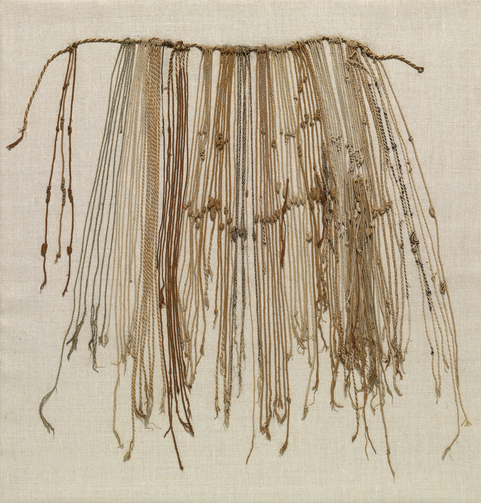
\includegraphics[scale=0.5]{quipu}
\caption{An incan quipu}
\label{quipu}
\end{center}
\end{figure}


Quipu were so successful that they remained the primary method of information processing in much of South America for thousands of years. They reached their peak of usage in the 15th century via the Inca empire. The Inca empire was the largest pre-Columbian empire in the western hemisphere, with over ten million subjects and spanning over two million square kilometers. Despite their intricate government, the Incas had {\em no written language}. This distinguished them from their contemporary empires, such as the Mali, Mongolian, or Chinese empires, which all relied on the written word. The success of the Inca empire can be seen as a testament to the versatility and power of knot invariants. The difference between the Inca and modern proposals for topological quantum computers is that instead of the strings being made out of cotton fibers they are made out of the spacetime trajectories of quasiparticles in topological systems.

Just like the history of topology in information science can be traced back to the origin of information science, the history of topology in quantum mechanics can be traced back to the origins of quantum mechanics. There is a 1931 paper of Paul Dirac \cite{dirac1931quantised} which introduces many of the ideas which would become foundational to topological quantum mechanics. In the 1950s, explicitly topological ideas such as the Aharanov-Bohm effect \cite{aharonov1959significance} and the theory of point defects by Tony Skyrme \cite{skyrme1962unified} were beginning to emerge. By the 1970s nontrivial abstract topological considerations were leading to novel contributions to contemporary physics, such as the theoretical description of the A-phase of superfluid Helium-3 \cite{anderson1977phase} and the theory of phase transitions in the xy model proposed by Kosterlitz-Thouless \cite{kosterlitz1973ordering}. These results were associated with the 1996 and 2016 Nobel prize respectively.

It was in the 1980s, however, that topology established itself as one of the leading themes in condensed matter physics. The discovery of the quantum Hall effect in 1980 \cite{klitzing1980new} and the subsequent discovery of the fractional quantum Hall effect in 1982 \cite{tsui1982two} gave the first examples of topologically ordered systems in our modern sense of the word, and resulted in the 1985 and 1998 Nobel prizes respectively. These systems gave theorists the license to dream big about what possibilities could lie ahead. This led to major work by Frank Wilczek \cite{wilczek1982quantum, arovas1985statistical}, Duncan Haldane \cite{haldane1983nonlinear, haldane1988model}, and others on the theory of topological quantum systems.

The most notable of these theorists for our present story is Edward Witten, with his introduction of {\em topological quantum field theory} in 1988 \cite{witten1988topological}. This work not only put the modern experiments within a larger context, but it also connected these developments to a parallel story which had been developing within pure mathematics. Namely, knot theory. In 1984 Vaughn Jones discovered his landmark knot invariant, which was powerful in its ability to distinguish between non-equivalent knots \cite{jones1997polynomial}. This marked the first major progress in the field since Alexander's invariant in 1928 \cite{alexander1928topological}. However, Jones’ construction was steeped in opaque subfactor theory, so much so that the fact that it resulted in knot invariant felt almost like a happy accident. Hence, a widespread topic on the mind of contemporary mathematicians was how to properly interpret the Jones invariant, and how to construct other invariants like it. Witten seemed to answer both. After defining topological quantum field theory, he showed how the Jones invariant could be obtained as an observable quantity within a certain field theory \cite{witten1989quantum}! This shocking result gave a new interpretation of the Jones invariant in terms of mathematical physics which was appealing to experts. Seeing as the Jones invariant was constructed from a topological quantum field theory, it was natural to expect that other field theories might give new invariants which could distinguish between even more knots. This vision of invariants in low-dimensional topology constructed using topological quantum field theory became known as {\em quantum topology}, and evolved into its own discipline in the following years.

This brings us to 1997. Quantum topology is an active area in pure mathematics, and topological themes in condensed matter physics are at the forefront of the field. The open problem is how to construct a fault tolerant quantum computer. Peter Shor had recently discovered his factoring algorithm \cite{shor1994algorithms}, and there was debate about whether scalable quantum error correction was possible \cite{landauer1995quantum}. This led to two independent proposals for topological quantum computation in the same year. One was by the mathematician Michael Freedman \cite{freedman1998p}. His vision was clear. A recent paper had shown that computing the Jones invariant of knots was in general an NP-hard problem \cite{jaeger1990computational}. However, by the work of Witten, the Jones invariants of knots were observables in certain topological quantum field theories. Hence, if one could construct physically a topologically ordered system which was described by Witten’s topological quantum field theory then the Jones polynomial of knots could be computed efficiently by making measurements on the system. Hence, one would obtain a very powerful computer! This was Freedman’s proposal.

The other proposal was made by theoretical physicist Alexei Kitaev \cite{kitaev2003fault}. His proposal was much more precise. He gave a toy model for a certain family of topologically ordered systems. He then outlined a technique for storing and manipulating information within these systems. The deep observation was that these systems were intricate enough that they could be used to make a powerful quantum computer \cite{mochon2003anyons}.

In the subsequent years Freedman and Kitaev teamed up with collaborators Zhenghan Wang, Michael Larsen, and others to study the new field of topological quantum information and the possibility of constructing a topological quantum computer. One of the first major results was that no topological quantum computer could be more powerful than a standard quantum computer \cite{freedman2002simulation}. This went against Freedman’s original hope to solve NP-hard problems using topological quantum computers. Freedman’s mistake was in asserting that topological quantum computers could compute the Jones polynomial. The measurements which give the Jones invariant in topological quantum field theory will always be {\em approximate}. Approximating the Jones invariant in this way is computationally easier than evaluating the Jones invariant exactly. In fact, this way of approximating the Jones invariant is \textit{not} NP-hard - it can only be used to solve problems which could efficiently be solved using standard quantum computers.

The second major result of Freedman, Kitaev, Wang, and Larsen was the converse of their first result \cite{freedman2002modular}. Namely, they showed that every quantum algorithm can be efficiently run on a topological quantum computer. They do this by showing that every quantum algorithm can be efficiently reinterpreted in terms of computing the Jones invariant of some knot. In this way computing the Jones invariant is not NP-hard, but it is a {\em universal problem} for quantum computation. They then formalize Freedman’s ideas about topological quantum field theory, and show directly that realistic operations on a topologically ordered quantum system described by Witten’s quantum field theory can be used to compute the Jones invariants of knots.

Together, these two results show in a real sense that topological quantum computing is equally powerful as standard quantum computing with circuits. This laid the groundwork for fruitful studies of fault-tolerant topological quantum computing, both using error correcting codes and physical materials. This has resulted in a great number of important results, which we will discuss at length throughout the rest of this manuscript.

\subsection{Technical introduction}
\label{technical-introduction}

\subsubsection{Principles of topological quantum information}
\label{principles-of-tqi}

In this section we will lay out the general principles of topological quantum information. As an organizational tool, these principles are introduced one by one as we construct a sample topological system. This example is meant to be representative of the systems we will encounter throughout this text, and within the broader field of topological quantum information. As a further organization tool, this example is constructed with the stated goal of obtaining a topological quantum computer.

Our system will be flat, containing only two spatial dimensions. Our system will be homogenous, essentially identical everywhere, at the exception of finitely many localized regions. These regions will differ substantially from the homogeneous bulk. These localized regions are called {\em quasiparticles}. The beauty of systems like these is that they behave as though the homogeneous bulk were empty, and the quasiparticles were fundamental particles. In fact, in its algebraic description, these topological systems are {\em identical} to ones in which the homogenous bulk is empty and the quasiparticles are fundamental particles. This is where the term quasiparticle arises. It is important however to remember that in most relevant applications the bulk is {\em not} empty and the quasiparticles are {\em not} fundamental particles. The bulk is typically some highly entangled quantum wavefunction, and the quasiparticles are emergent phenomena made up of smaller microscopic degrees of freedom.

\begin{figure}[h]
\begin{center}
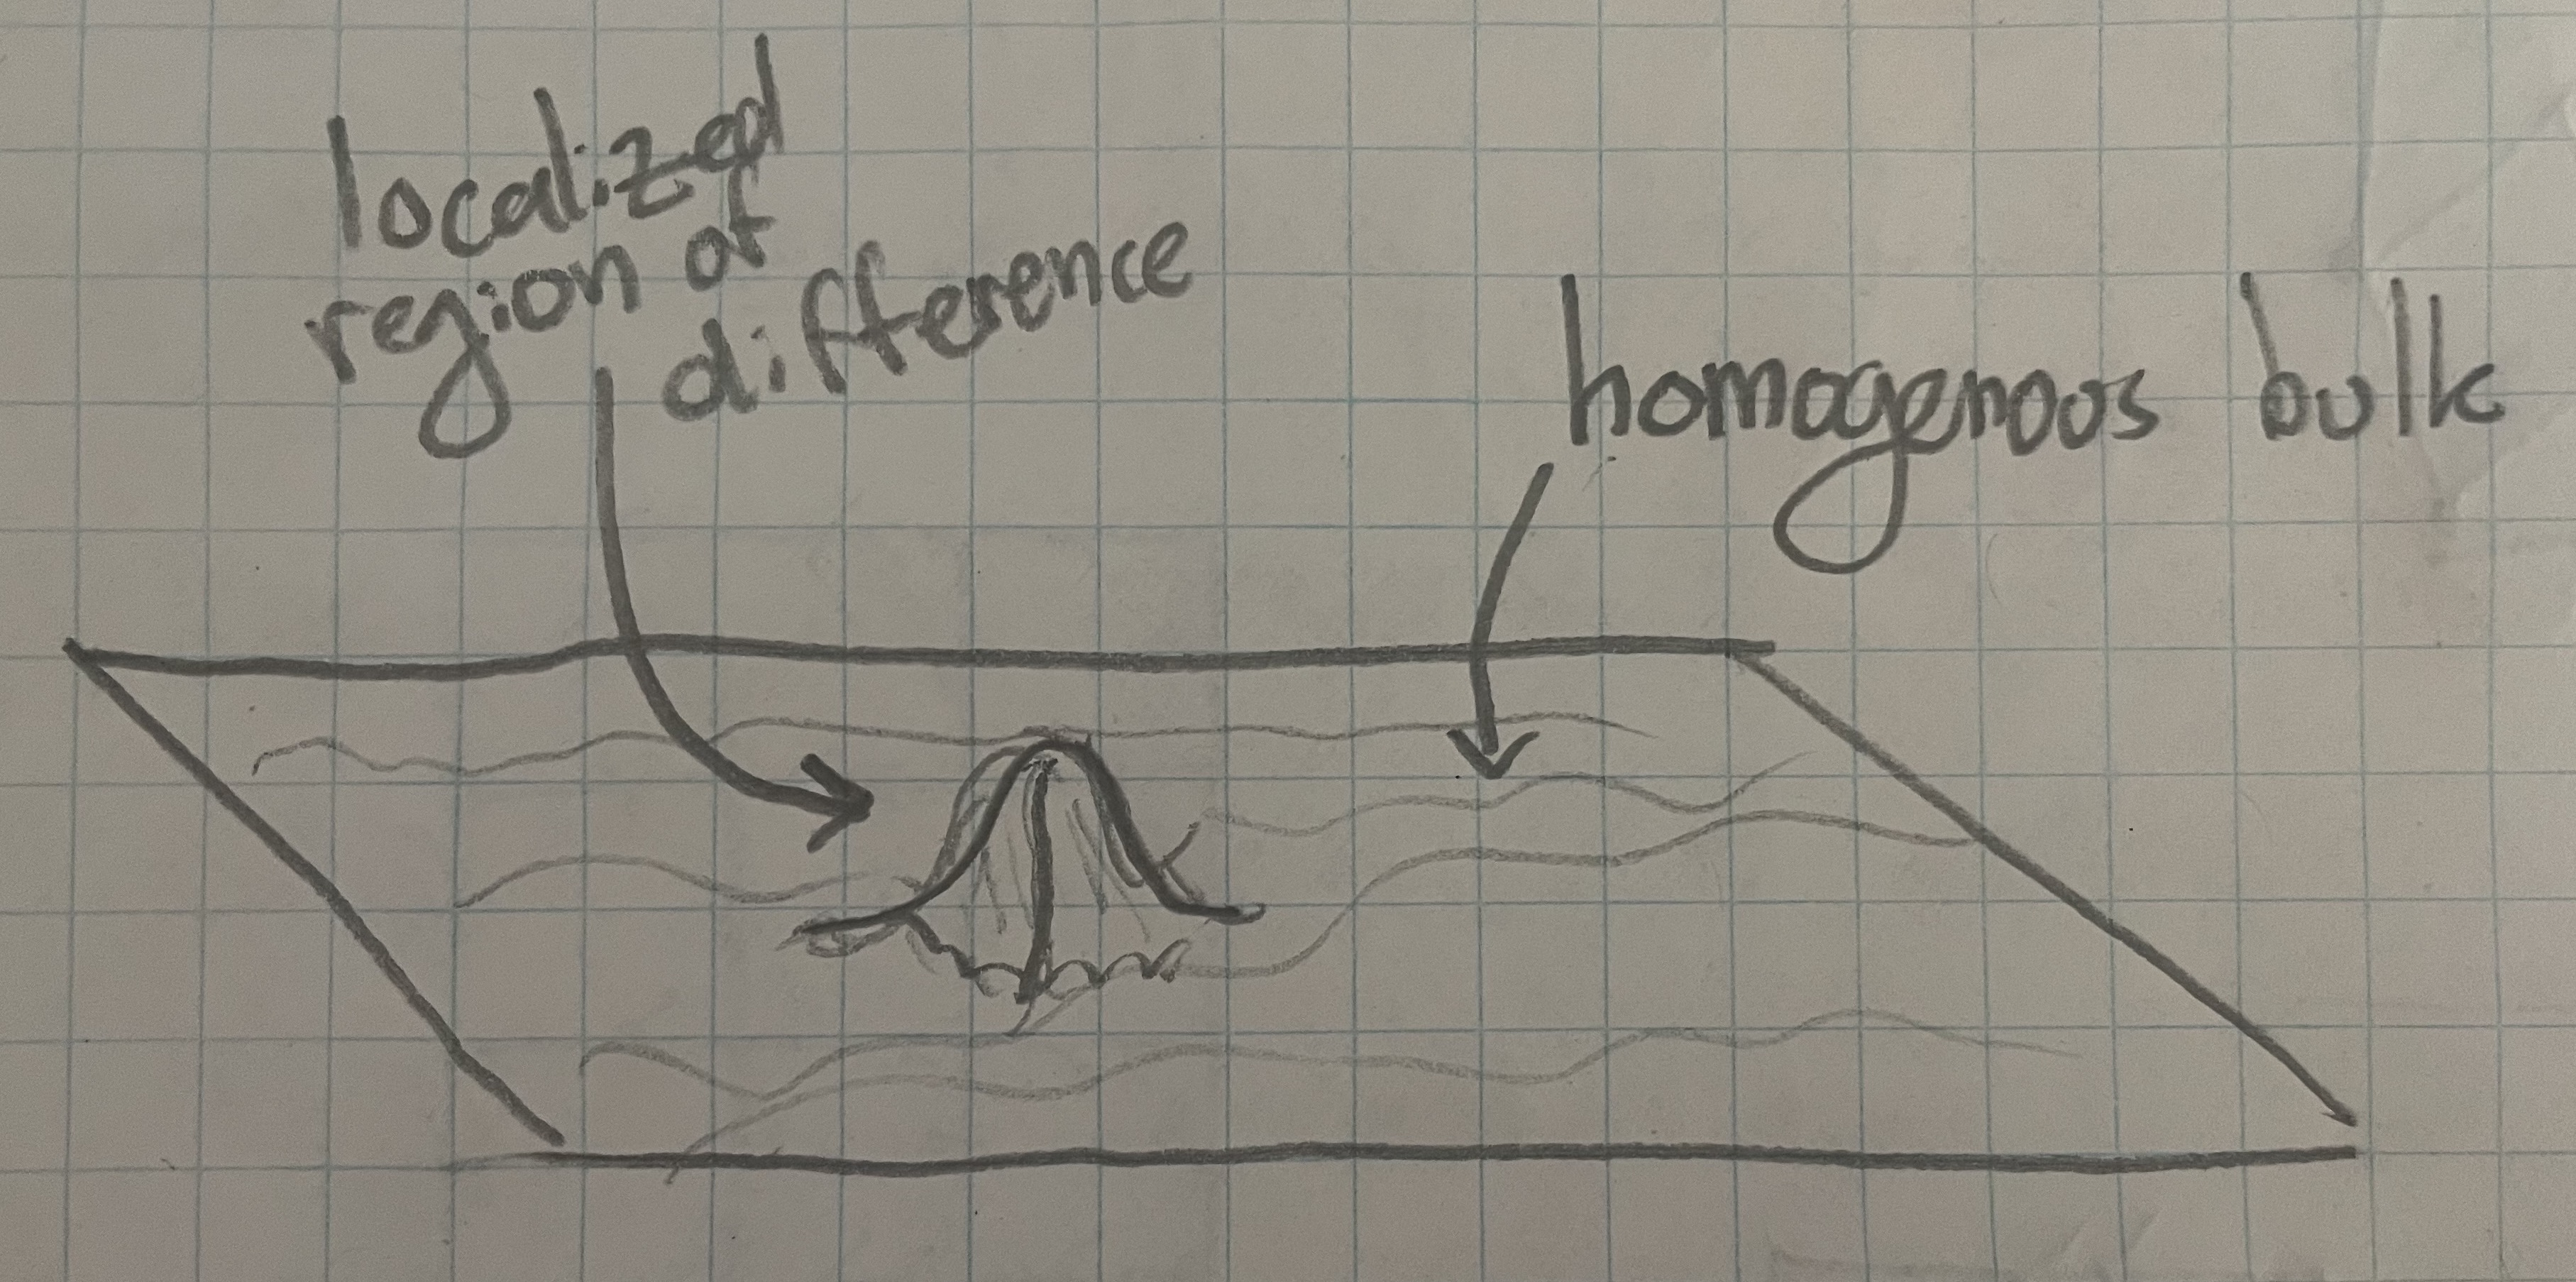
\includegraphics[scale=.04]{quasiparticle}
\end{center}
\caption{A quasiparticle in a two dimensional system}
\end{figure}

Our aim is to build a computer. In general this requires three components:

\begin{enumerate}
\item A method of storing information;
\item A method of manipulating information;
\item A method of reading out information.
\end{enumerate}

Information is stored in the state of the system - the bulk is described by some parameters, and the details of those parameters encodes information. Our method for manipulating information is {\em braiding}. Braiding is the process whereby quasiparticles are moved along continuous paths around one another. There are two important points about braiding to keep in mind. The first is that braiding changes the state of the system. Even though the quasiparticles might be in identical places before and after the braid, the details of the system will change - there is more to the state of the system than just the positions of the quasiparticles. The second point is that the way that the state of the system changes {\em only depends on the topology of the braid}, and not the geometry. Small deformations in the path taken by the quasiparticles do not affect the result - only global changes, like whether a path is taken clockwise or counterclockwise, make a difference. This invariance is due to the fact that our system is topological. In geometric systems we expect the exact path taken by quasiparticles matters a great deal. The independence of the details of the paths is extremely specific to topological systems, and in the present setting is the {\em defining feature} of a topological system.

\begin{figure}
\begin{center}
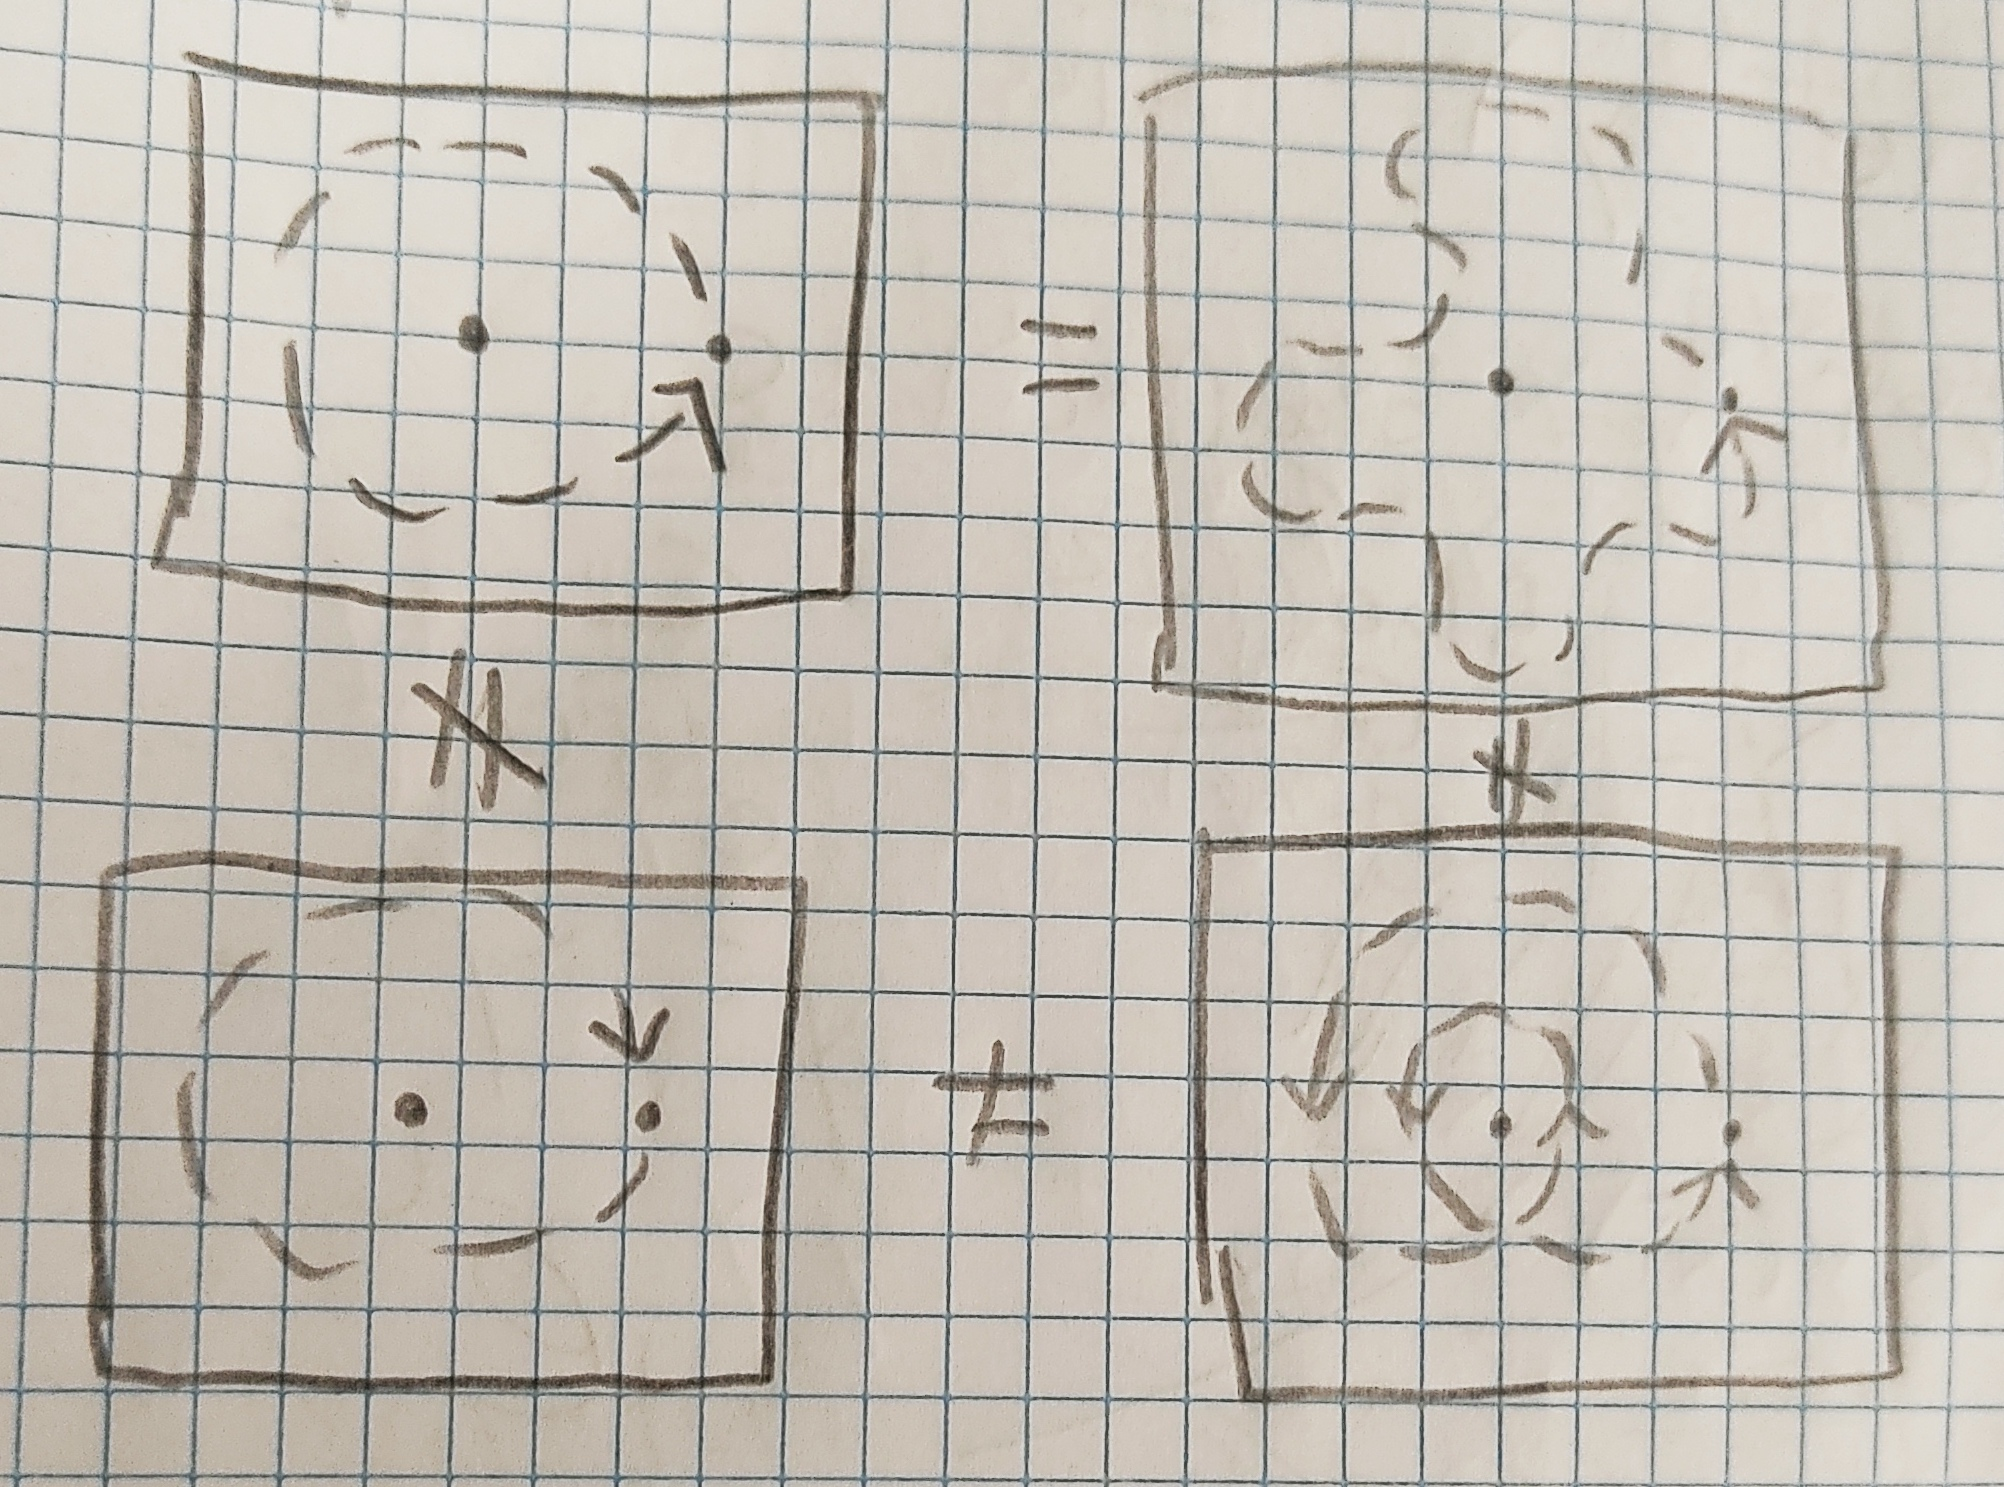
\includegraphics[scale=0.065]{braid-topologies}
\caption{Samples of braids quasiparticles can take around one another}
\label{braid-topologies}
\end{center}
\end{figure}

At this point we can already see we have succeeded in our goal of making our computations fault-tolerant. Noise in the system will correspond to uncontrolled perturbations in the trajectories of the quasiparticles. This uncontrolled movement won’t change global properties of paths taken, and hence will not change the action of the braids on the system. That is, small errors won't affect computation! Of course, large enough errors could unintentionally make one quasiparticle wind around another. This would change the topology of the braid and hence ruin the computation. These errors are controllable, however, by moving the quasiparticles far apart and limiting the magnitude of the noise.

The final step in making our computer is to introduce a method for reading out information. This is done using {\em fusion}. Fusion is the process whereby two quasiparticles are brought together, resulting in a single quasiparticle. In sufficiently complicated topological systems the result of fusion depends on the details of the state of the overall system. That is, the result of fusion can be used as a way of reading out information about the state! In its most basic form, when two quasiparticles fuse they can either result in a localized region which is identical to the homogenous bulk or is different from the homogenous bulk. If they result in a localized region identical to the bulk we say that the two quasiparticles have {\em annihilated} each other. This can be seen as the difference between constructive and destructive interference. Two waves can either have destructive interference and annihilate each other when they meet, or they can have constructive inteference and result in a new wave. Measuring whether or not two quasiparticles annihilate upon fusion gives a method for reading out information.

In some situations, the result of fusion can even be nondeterministic. In this case the fusion can be repeated multiple times, which allows one to measure the {\em probability} that two quasiparticles will annihilate each other. These probabilities are a rich source of data, and will serve as our way of reading out information in the current setting. The fact that our system is topological implies that the result of fusion does not depend on the specifics of the path taken, and hence this method of readout preserves the invariance of our computation to noise. This gives us a full picture of topological quantum computation, as seen in figure \ref{TQC-outline}.

\begin{figure}
\begin{center}
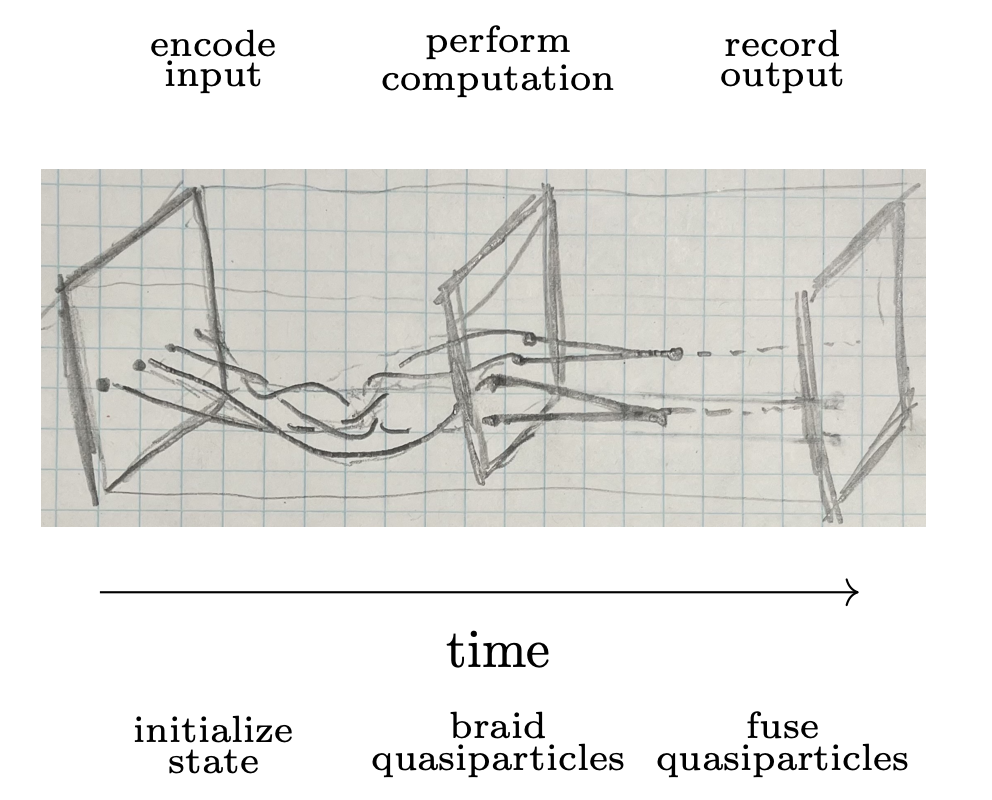
\includegraphics[scale=0.35]{TQC-outline}
\caption{A schematic of topological quantum computing}
\label{TQC-outline}
\end{center}
\end{figure}

\begin{ex}
To make the above discussion more concrete, we will give a worked example. In this example we use a specific topological order known as the {\em Fibonacci particle theory} to run Shor’s efficient quantum factorization algorithm \cite{shor1994algorithms}. The input of Shor’s algorithm is a positive integer. The output of Shor’s algorithm is the factorization of that integer. Shor’s algorithm is {\em efficient} in the sense that it uses polynomially many quantum logic gates to arrive at its answer relative to the size of the input. Throughout this passage we will use {\em efficient} and {\em polynomially sized} interchangeably. The Fibonacci particle theory is a specific topological order, which describes in an algebraic fashion how the overall state changes when quasiparticles are braided and fused.

The first step in running Shor’s algorithm on a Fibonacci quantum computer is to translate the positive integer input into a certain braid. This is done using an efficient classical algorithm. The second step is to run this braid on a Fibonacci quantum computer. This is done by initializing some prescribed state and then braiding its quasiparticles in the correct fashion. This initialization and braiding is performed repeatedly, and after every time two of the quasiparticles are fused. This lets us record a real number between 0 and 1, which is the probability that the two quasiparticles annihilate after the braiding. An efficient classical algorithm is then used to take this real number and obtain from it the factorization of the original input. Since all of these steps are efficient, it gives a topological quantum algorithm for factoring integers. The schematic for this process is shown below:

\begin{equation*}
\tikzfig{shor-fibonacci}
\end{equation*}

The magic in the above procedure is the existence of these two efficient classical algorithms: a first one for encoding integers into braids and a second one for decoding real numbers into factorizations. These algorithms are nontrivial. They are due to Freedman-Larsen-Kitaev-Wang \cite{freedman2002modular}. In fact, Freedman-Larsen-Kitaev-Wang showed that any problem which can be efficiently solved using a quantum circuit can also be solved using the Fibonacci particle theory, via a similar method of efficient classical preprocessing and postprocessing. It is in this sense that the Fibonacci theory is {\em universal} for quantum computation.
\end{ex}

To make a real topological quantum computer, one would need to create a physical topological system which is described by the Fibonacci theory. In the realm of materials, the most promising approach seems to be specially tuned versions of the fractional quantum Hall system \cite{zhu2015fractional}. While these materials are theorized to host quasiparticles described by the Fibonacci theory, the difficulty of the experiment makes them inaccessible to current technology. There has been progress made on topological quantum error correcting codes which work by simulating the Fibonacci theory \cite{schotte2022quantum, schotte2022fault, xu2024non}. However these codes at the current moment have structural issues and require an unbearable amount of overhead to run, making them unfeasible to use on modern computers.

Progress on topological quantum computing has thus been focused on realizing topological particle theories other than the Fibonacci theory. These other theories can be constructed in more workable materials, and can be simulated as topological quantum error correcting codes with less overhead. The drawback of these other theories is that they are typically less computationally powerful, meaning that they require more tricks and techniques to achieve universal quantum computing. There are a great number of different proposals for how to achieve universal topological quantum computing, based on different particle theories, different methods of encoding information, different methods of manipulating information, and different methods of reading out information. It is an exciting time to be a theorist in the field of topological quantum information!

\subsubsection{Defects in ordered media}

We will now work through a complete mathematical example of a family of topological systems. Seeing as we don't assume that the reader is familiar with quantum mechanics, our examples will be {\em classical} topological systems. Many of the important subtleties of topological quantum information are already present in the classical case. However, topological classical information is a smaller domain than topological quantum information - the reader should have a relatively complete grasp of the subject by the end of the chapter. Much of our discussion is taken from an excellent review article by Mermin \cite{mermin1979topological}.

The family of systems we will describe goes by many names. In communities of experimentally focused physicists it goes by the name {\em ordered media}. In mathematical physics communities it goes by the name {\em classical field theory}. In pure mathematics it would be described as {\em homotopy theory}. As an input to our construction we will take a topological space called the {\em order space} of our theory. To simply notation, we fix the convention

$$M\text{ is a path-connected topological space, the order space.}$$

To describe a system in physics, the first step is to define the space of possible states of the system. In this case, states will correspond to {\em continuous maps $\phi: \bR^2\to M$}. We now give physical intuition for this choice of state space. The choice of $\bR^2$ as a source represents the underlying material. We are working on an infinite flat plane. Describing a function $\phi: \bR^2\to M$ amounts to choosing a value $\phi(x)$ for every point $x\in \bR^2$. In this way we imagine our system as being made up of infinitely many objects, one placed at each point in $\bR^2$, each of which has an internal state space $M$. Choosing the state of the overall system amounts to choosing the state of each individual object, that is, a value in $M$ for every point in the plane. The fact that $\phi$ must be continuous is a compatibility condition between the states of the objects at nearby points. It says that nearby objects must have similar states. We now list some applications of this model:

\begin{itemize}
\item {\bf Classical xy model of a 2D electron gas} (\cite{kosterlitz2018ordering}). This model describes a possible behavior electrons in a flat 2D plane. An electron can be modeled as a point particle with a magnetic dipole pointing in some direction. This magnetic dipole is known as the \textit{spin} of the election, and can point in any direction in the plane. The topological space of all possible directions in the plane is a circle. Hence, in this system, the order space $M$ is the circle. The fact that nearby electrons must have similar spins is known as Hund’s rule, and is the most fundamental incarnation of ferromagnetism. It is physically derived as a consequence of the Pauli exclusion principle.

\item \textbf{Superfluid Helium-3} (\cite{lee1997extraordinary}). One famous example of ordered media is superfluid helium-3. Helium is an element. It has two stable isotopes: helium-3 and helium-4. The vast majority of helium on earth is helium-4, but there is also naturally occuring helium-3. At cold temperatures helium-3 undergoes a phase transition, becoming a superfluid. There are several different superfluid phases helium-3 can go into: the B-phase, dipole-locked A-phase, and dipole-free A-phase. The dipole-locked A-phase is well modeled by ordered media with order space $M=\SO(3)$, where $\SO(3)$ is the space of rotations in three dimensional space. The dipole-free A-phase is well modeled by ordered media with order space $M=\SO(3)\times \SO(3)/H$, where $H$ is the subgroup of $SO(3)\times SO(3)$ generated by rotations across the $z$-axis of any degree, and simultaneous rotations of $180^\circ$ on both copies of $\SO(3)$ around any axis.

\item \textbf{Biaxial nematics} (\cite{ranganath1988defects}). The objects at every point in the biaxial nematic should be thought of as small rectangles with unequal side lengths. These rectangles can be oriented in any direction in three dimensional space. In practice these objects will often be molecular compounds. They will not be exactly rectangular, but they will have the same symmetry group as a rectangle which is enough for the model to be accurate. The order space $M$ of the model is equal to the space of possible orientations of a rectangle in three dimensions. Note that in this space every orientation is equal to its $180^\circ$ rotation across any axis of the rectangle, since the rectangle is symmetric under such rotations.
\end{itemize}

\begin{figure}
\begin{center}
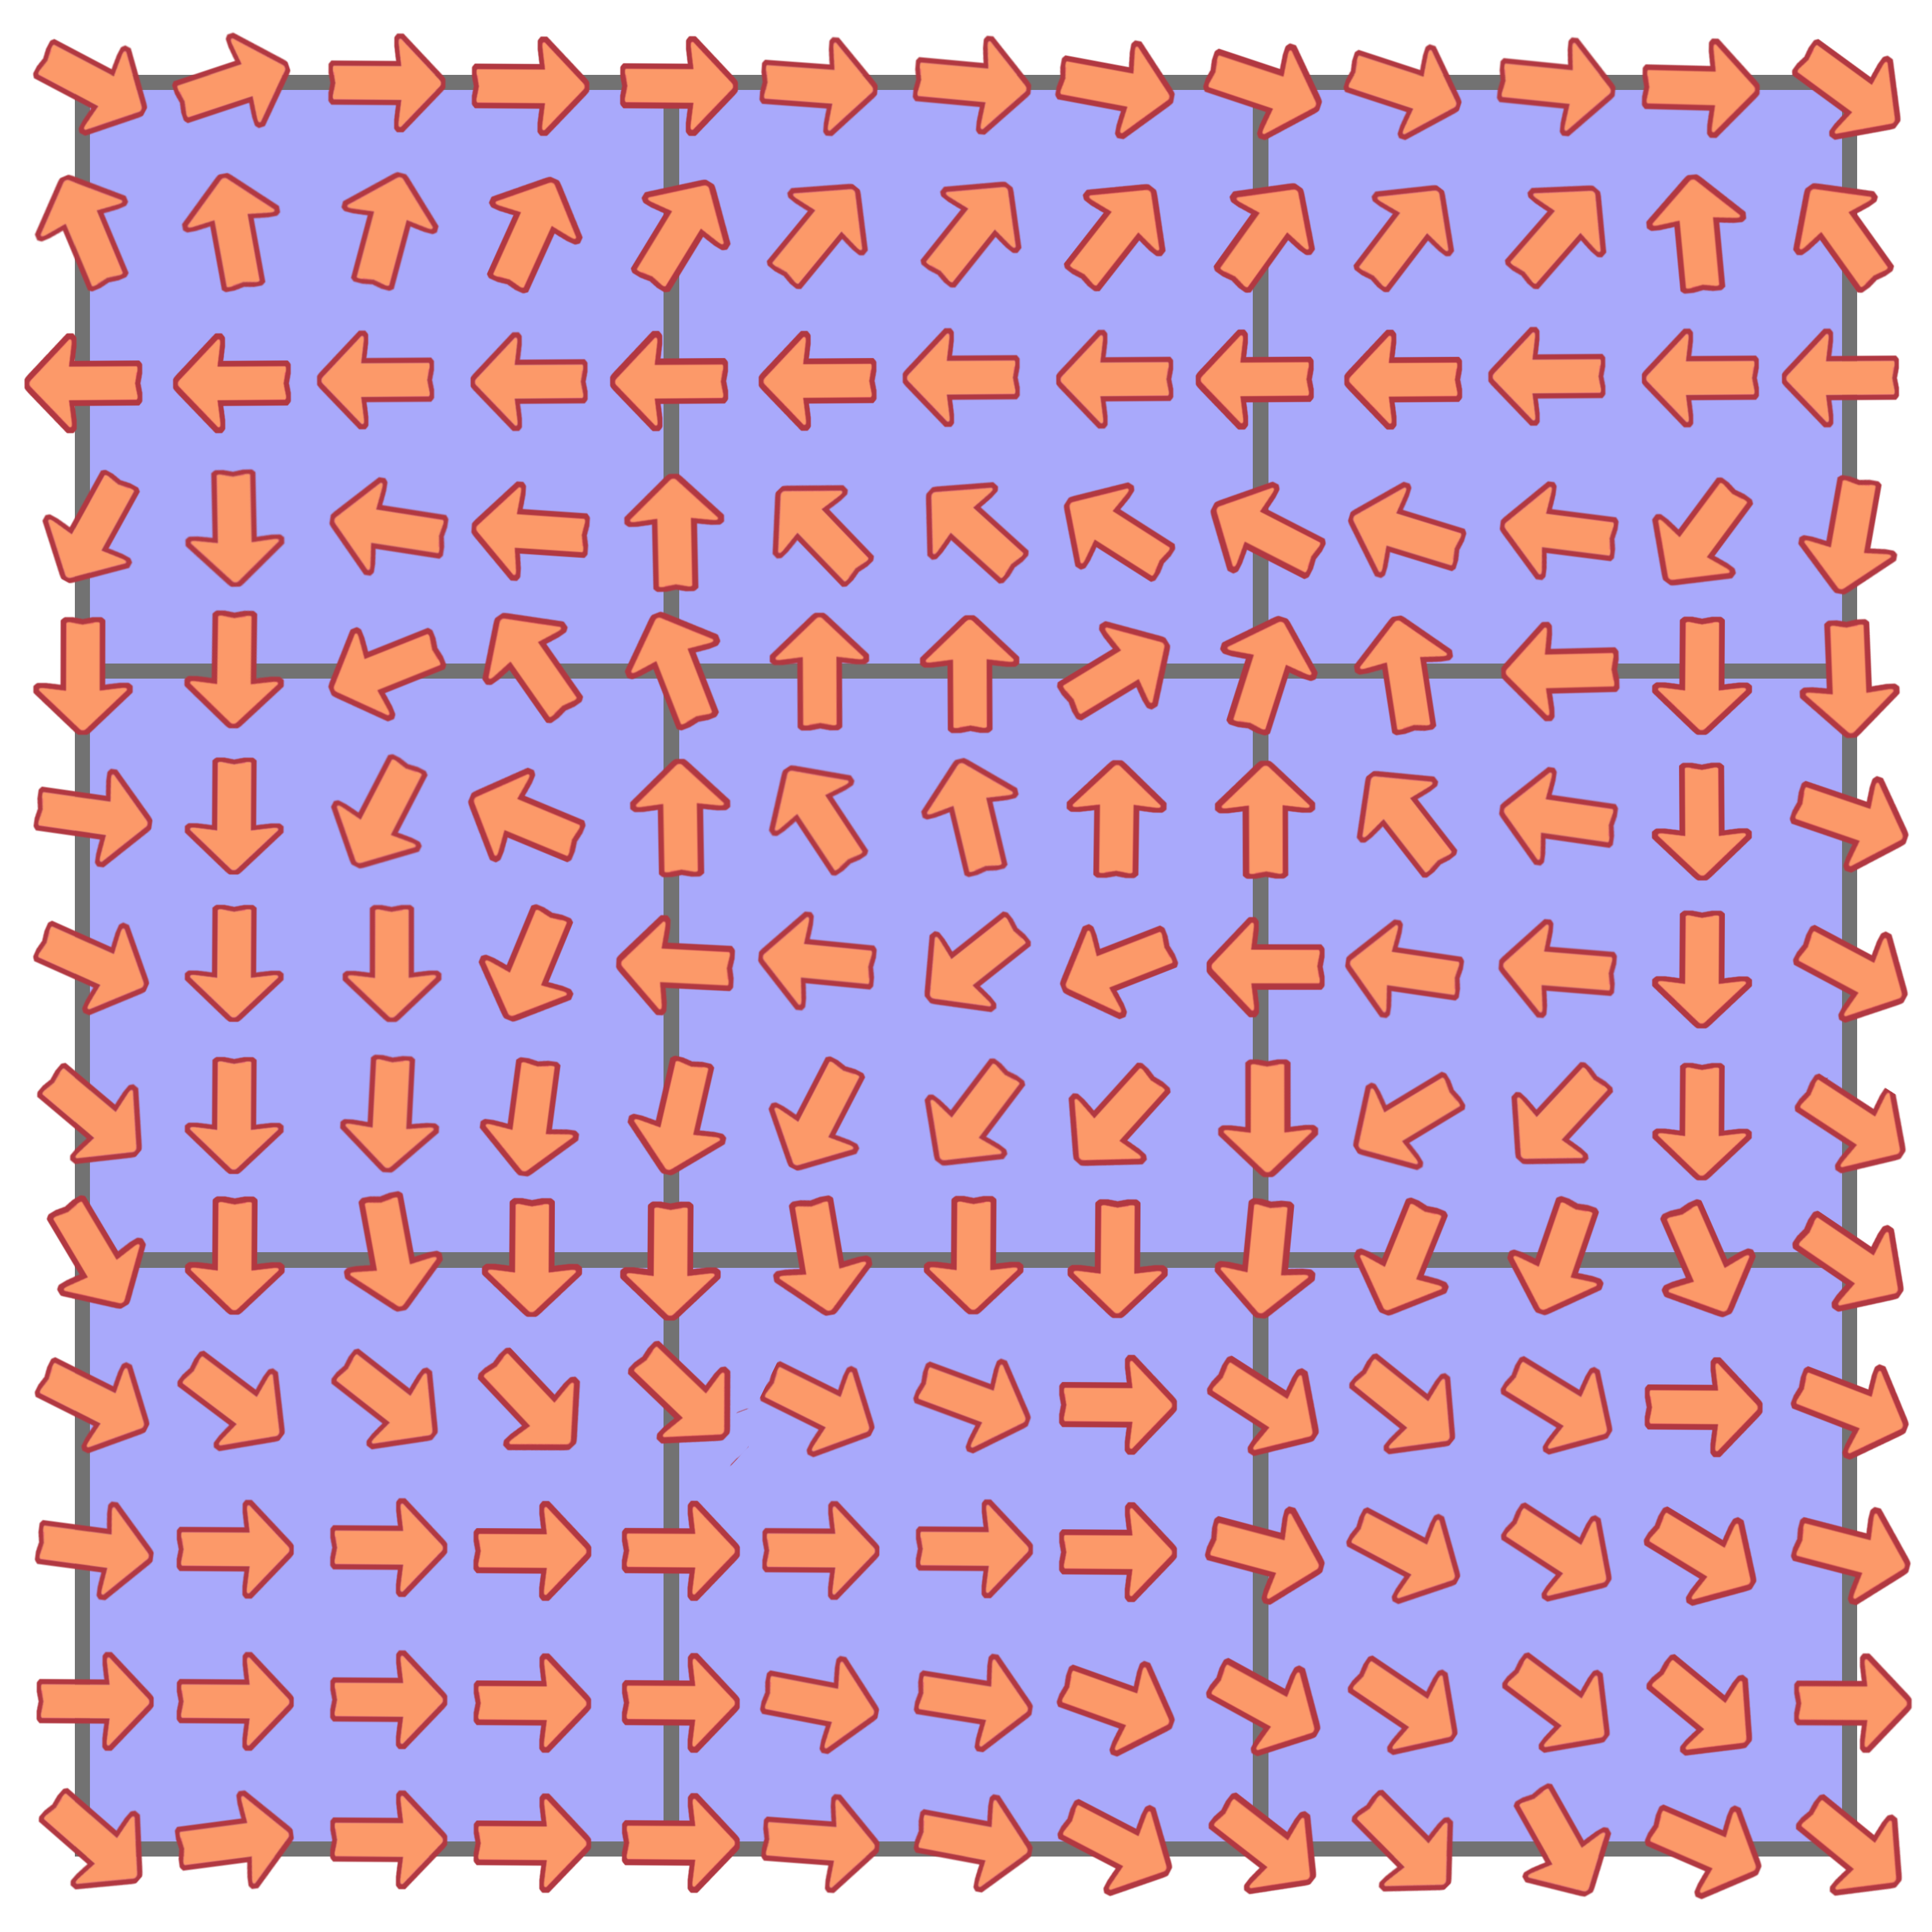
\includegraphics[scale=0.04]{xy-model}
\caption{The xy-model of a 2D electron gas}
\label{xy-model}
\end{center}
\end{figure}

We now seek extend our model of ordered media and perform a detailed analysis of it. To do this, we will need to use notions from topology such as a {\em continuous deformation} of a system and the \textit{inside} of a loop in $\bR^2$. While these notions are certainly intuitive, they can be shockingly hard to prove. The fact that every loop in $\bR^2$ partitions space into an {\em inside} and an {\em outside} is known as the Jordan curve theorem. The proof of this trivial seeming statement is famously tricky \cite{tverberg1980proof}. Thus, we adopt the following policy:
$\newline$

\fbox{\parbox{\dimexpr\linewidth-2\fboxsep-2\fboxrule\relax}{
Seeing as the primary focus of this text is algebra we opt to leave our topology non-rigorous, focusing instead on principles and techniques. We only return to mathematical rigor once the subject has become sufficiently algebraic.
}}

$\newline$
We now add a picture of {\em dynamics} into our model - how states will be change through time. In particular, we imagine that as time passes the system changes continuously. Suppose that $\phi_t:\bR^2\to M$ is the state of the system at time $t$. If $t_0$, $t_1$ are similar times we require $\phi_{t_0}(x)$ and $\phi_{t_1}(x)$ will be close. Formally, we say that a family of states $\phi_t$ for $0\leq t \leq T$ form a valid trajectory in time if the map

\begin{align*}
\phi_{\cdot}: \bR^2\times[0,T]&\xrightarrow{} M\\
(x,t)&\mapsto \phi_t(x)
\end{align*}

is continuous. We also call $\phi_{\dash}$ a continuous deformation from $\phi_0$ to $\phi_T$, because the trajectory in time continuously changes the initial state $\phi_0$ until it becomes the final state $\phi_T$.

\begin{rem}\label{no-topological-information}
It is a general fact from topology that every pair of maps $\phi_0,\phi_1: \bR^2\to M$ can be continuously deformed from one to the other. Intuitively, this means that as our system evolves it can transition continuously from any state to any other state. In this way, our system does not store any information which is invariant under continuous deformations. That is, it does not hold any {\em topologically invariant} information.
\end{rem}

In light of remark \ref{no-topological-information}, we find our ordered media system is not complicated enough to build a computer yet because it cannot store information. We rectify this situation by introducing quasiparticles. These quasiparticles go by many names. In the theory of ordered media they are known as defects. In field theory they are known as particles. In homotopy theory they are known as point singularities. For the sake of brevity, we use the term defect.

A defect is a point at which we drop our condition that the state $\phi:\bR^2\to M$ be continuous. This is done by making $\phi$ {\em undefined} at certain points. Our new system is called {\em ordered media with finitely many defects}. The state space consists of pairs $(S,\phi)$, where $S\subset \bR^2$ is a finite set and $\phi: \bR^2\backslash S\to M$ is a continuous map.

\begin{figure}
\begin{center}
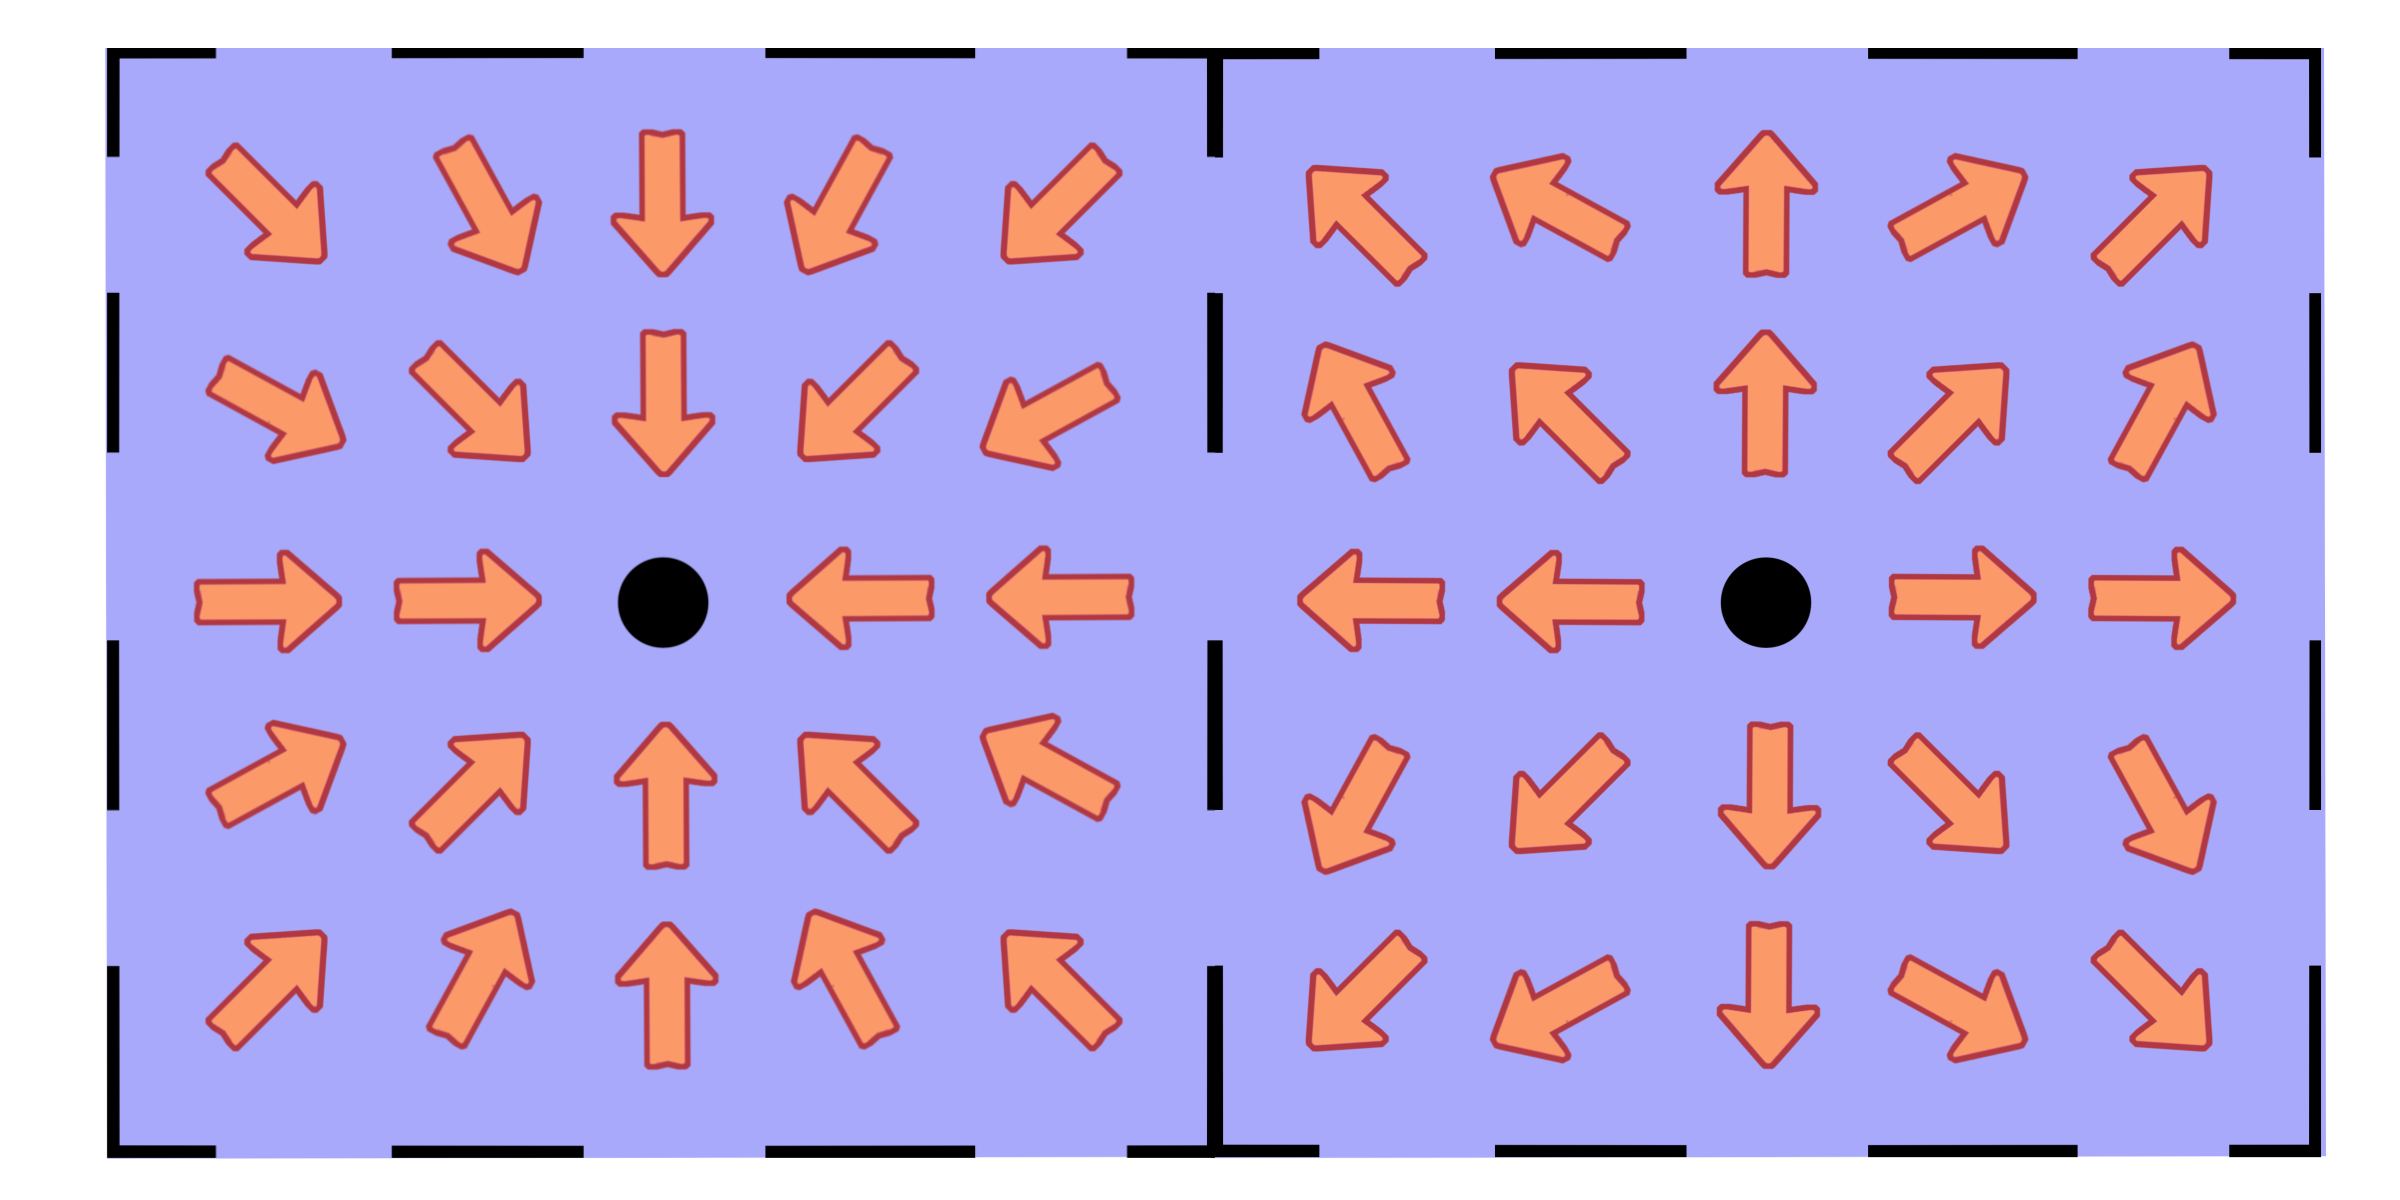
\includegraphics[scale=0.06]{xy-defects}
\caption{Two defects in the xy-model}
\label{xy-defects}
\end{center}
\end{figure}

Dynamics in our new system still correspond to continuous deformations. The subtelty now is that the defects can move as the state is deformed. We call these {\em defect-mobile deformations}. Following our general stance on topological rigor, we omit the precise definition of defect-mobile deformation. 

The vision for building our computer is that the experimenter should have control of the trajectories of the defects, but no control over the rest of the system. This means that the system will trasform under defect-mobile deformations with definite defect paths chosen by the experimenter, but the details of the rest of the deformation is arbitarily and uncontrollable. The principle that the details of the deformation are uncontrollable comes from the fact that we expect the individual objects making up the ordered media to by noisy - the are prone to uncontrolled transformations and errors. The defects, however, are made up of many objects and are stabilized by the assumption that there is a physical mechanism which forces most nearby objects to have similar states.

We can now outline the big idea of how the computer will work. We will arrange $n$ defects on a line in the plane. We keep these defects still, so that the system is changing only by deformations which keep the defects in place. We call these {\em defect-fixed deformations}. We store our information in the possible topologically-distinct states of this system:

\begin{equation*}
\left(\substack{
\text{information storage} \\ \text{space}}\right)
=
\left.\left(\substack{
\text{states with $n$ defects} \\ \text{arranged in a line}}\right)\right/
\left(\substack{
\text{defect-fixed} \\ \text{deformation}}\right)
\end{equation*}

\begin{figure}
\begin{center}
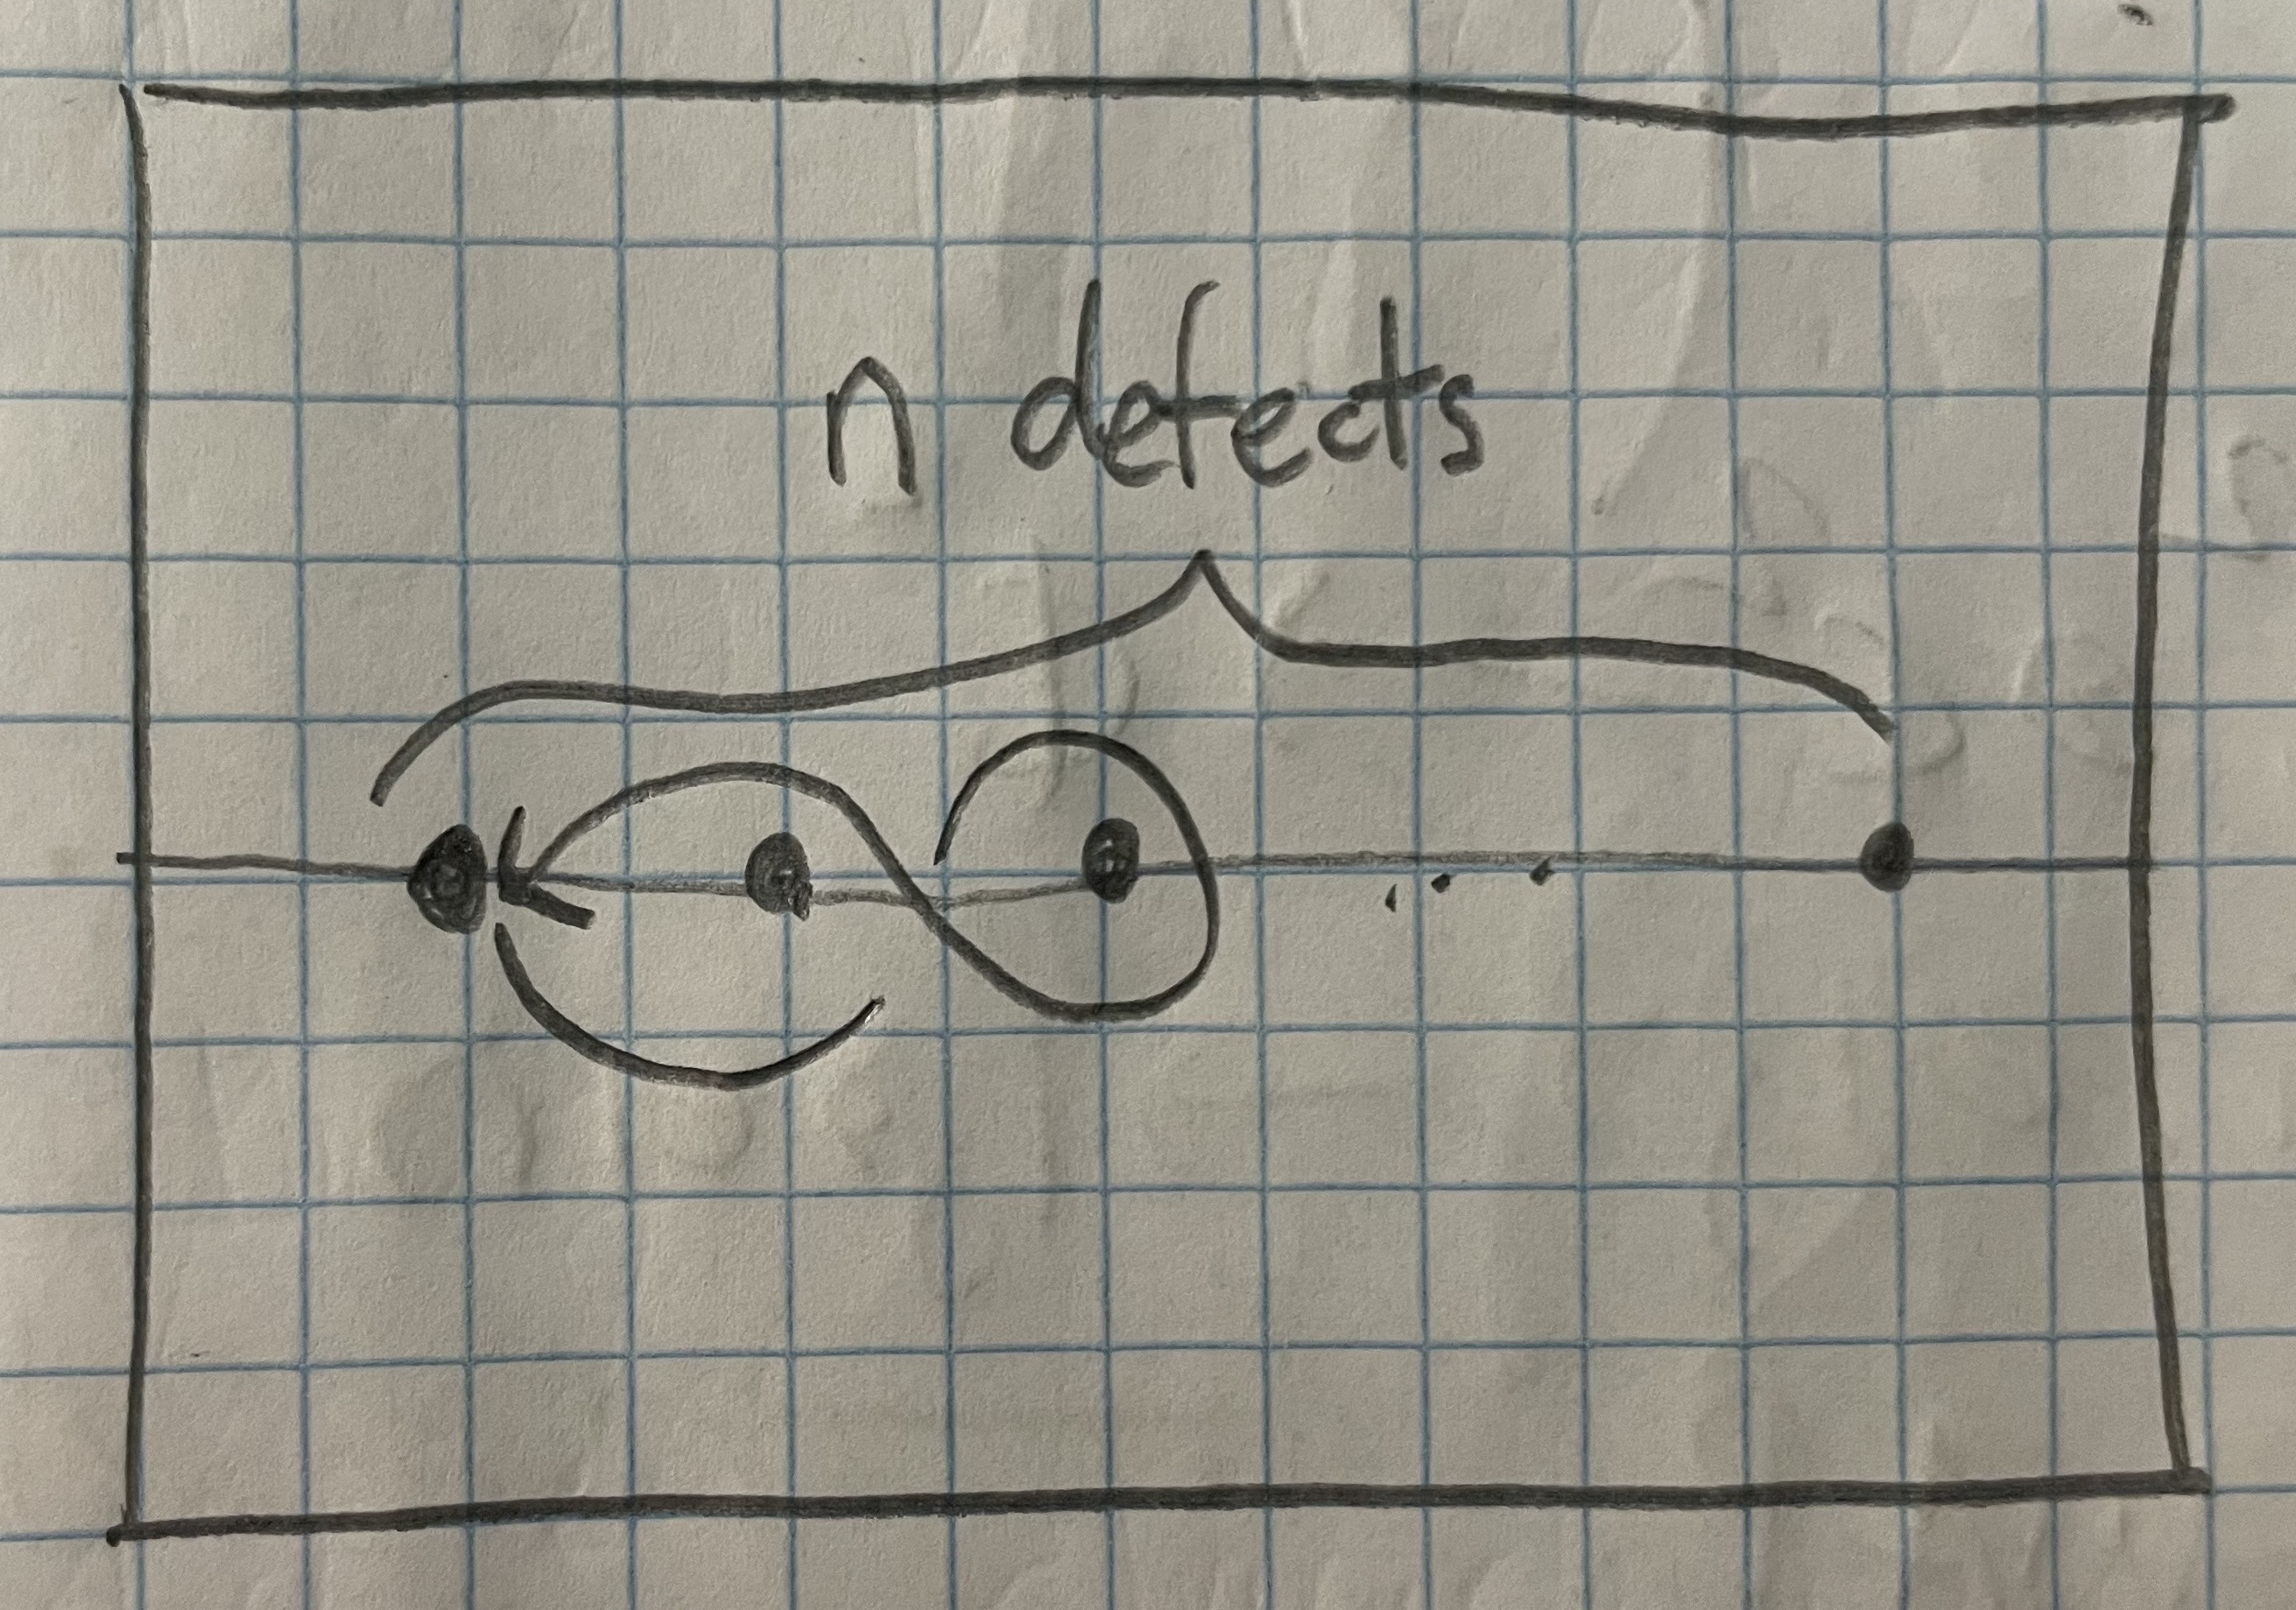
\includegraphics[scale=0.05]{defects}
\caption{Defects on a line, with a sample trajectory of one particle around the others.}
\label{defects}
\end{center}
\end{figure}

The way we act on this information is by moving the defects around each other. This movement of defects induces some defect-mobile deformation. The space we are storing our information in is invariant under defect-fixed deformation, but not defect-mobile deformations. Hence, moving the defects around non-trivial paths will have non-trivial action on the stored information. This action on stored information is exaclty how we perform our computations.

Finally, we must introduce a method for reading out information. This is done via fusion. Two defects can be brought together and fused. The result of this fusion is a topologically invariant quantity, and we will assume that it can be measured by an experimenter. In its most simple form, this amounts to detecting whether two defects annhilated or not.  This gives us some information about the state, which is the output of our computation. This process is described visually in Figure \ref{TQC-outline}

In the rest of this chapter we will describe exactly what the space we are storing our information in looks like, how braids act on that information, and how this can be used to make a functioning computer. This will give a detailed picture of how topological computation works.

\subsubsection{The fundamental group}
\label{the-fundamental-group}

To understand topological computation we will need to put in some real work analysing defects in ordered media. Our main technical ingredient will be a construction from topology known as the {\em fundamental group}. In this section we will define the fundamental group and apply it to ordered media.

The fundamental group is derived from a careful analysis of loops in topological spaces. We first clairfy what we mean by {\em loop}. Loops, for our purposes, are always oriented and are allowed arbitrary self intersections. Formally, we define a loop in a topological space $M$ to be a continuous map $\alpha:[0,1]\to M$ such that $\alpha(0)=\alpha(1)$.

\begin{figure}
\begin{center}
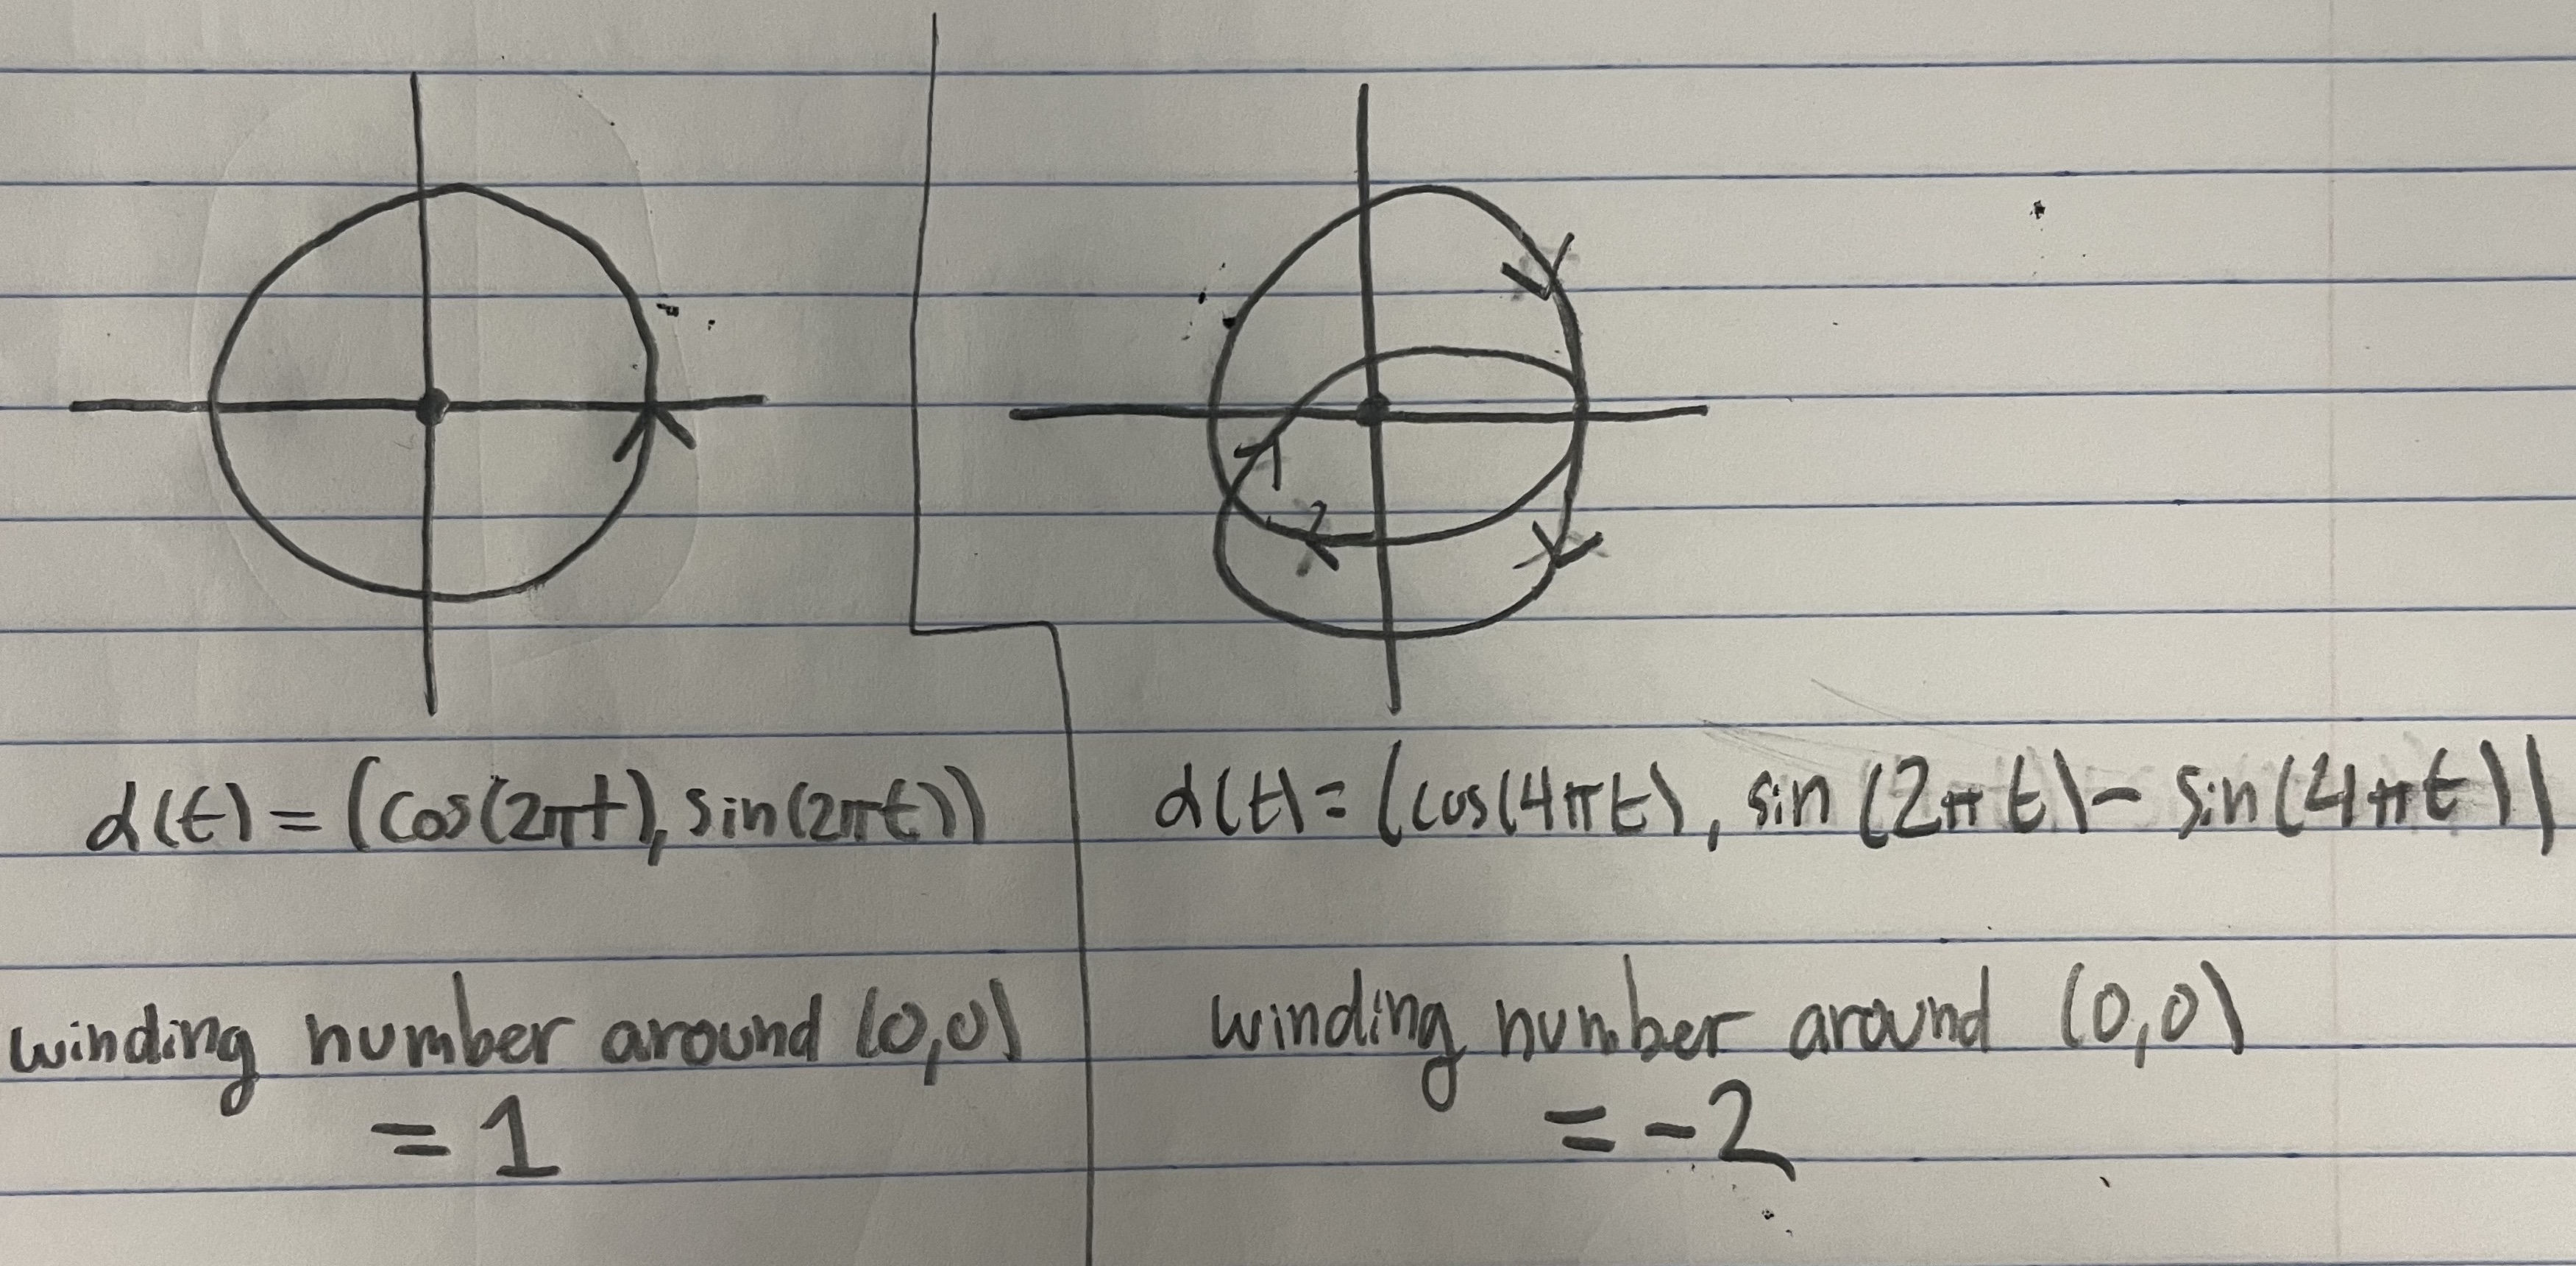
\includegraphics[scale=0.06]{loops}
\caption{Examples of loops in $\bR^2$.}
\label{loops}
\end{center}
\end{figure}

A clever observation is that the space of loops can be endowed with the structure of a group. A group, by definition, has a group operation. A natural choice of group operation on the space of loops is {\em composition}. Given two loops we can compose them by first following one loop and then following the other.

Importantly, composing loops has a subtlety. To compose, we glue the endpoint of one loop to the start point of the other. However, loops do not have marked start and end points so this composition rule is not well-defined! To fix this issue, we work with loops that do have a distinguished start and end point. Formally, we define a {\em based loop} in a topological space $M$ to be a pair $(\alpha,m)$ where $m\in M$ is a point known as the {\em basepoint} of the loop, and $\alpha:[0,1]\to M$ is a continuous map such that $\alpha(0)=\alpha(1)=m$. The composition of based loops is well-defined. Given two based loops $\alpha_0,\alpha_1$ in $M$ with basepoint $m\in M$, we define their composition to be

$$
(\alpha_1 \circ \alpha_0)(s)=
\begin{cases}
\alpha_0(2s) & 0\leq t \leq 1/2 \\
\alpha_1(2(s-1/2)) & 1/2 < t \leq 1.
\end{cases}$$

The reason we need to add the factors of two is to ensure that the domain of the loop is still the unit interval $[0,1]$. Intuitively, to fit two loops in the same amount of time we had to speed-up both by a factor of two. This composed map is continuous at $s=1/2$ because the left and right limits of $(\alpha_1 \circ \alpha_0)(s)$ are both equal to $m$.

Despite being well-defined, composition does {\em not} endow the space of based loops in a topological space with the structure of a group. The issue that the axioms of associativity, unit, and inverse all fail to hold. A clever way to fix these problems and to make the resulting group more universal is to only consider equivalence classes of based loops up to deformations which preserve the basepoint. This means that if there is a continuous deformation between two loops which leaves the basepoint fixed along the entire deformation, then the two loops are considered to be equivalent. It is not difficult to verify that the composition rule for based loops is well-defined on such equivalence classes, and gives rise to the {\em fundamental group of a topological space $M$ with basepoint $m\in M$}:

$$\pi_1(M,m)\coloneqq \left(\text{loops in $M$ based at $m$}\right)/\left(\text{basepoint preserving deformations}\right).$$

We denote the equivalence class of the based loop $\alpha$ by $[\alpha]\in \pi_1(M,m)$. The identity element in the fundamental group is the equivalence class of the trivial loop $\alpha(s)=m$ which stays at its basepoint and doesn't move. Inverses are given by reversing orientation. That is, the inverse of $[\alpha]$ is the equivalence class of $\alpha^{-1}(s)=\alpha(1-s)$.

\begin{ex}
The good first fundamental group to compute is $\pi_1(\bR^2,0)$. Suppose that $\alpha$ is a loop in $\bR^2$ based at $0$. The define $\alpha_t(s)=t\cdot \alpha(s)$ for $0\leq t\leq 1$. The maps $\alpha_t:[0,1]\to \bR^2$ are loops based at $0$ becasue $\alpha_t(0)=t\cdot \alpha(0)=0$ and $\alpha_t(1)=t\cdot \alpha(1)=0$. Hence, the family of loops $\alpha_t$ provides a basepoint preserving deformation from $\alpha_1=\alpha$ to the constant map $\alpha_0=0$. Hence, all loops in $\bR^2$ based at $0$ are equivalent to the constant map in the fundamental group so $\pi_1(\bR^2,0)=0$. Applying translations, we find more generally that $\pi_1(\bR^2,m)=0$ for any $m\in \bR^2$.
\end{ex}

\begin{ex}
Another important important fundamental group to compute is $\pi_1(\bR^2\backslash\{p\},m)$ for distinct points, $p,m\in \bR^2$. Every loop $\alpha$ in $\bR^2$ goes around $p$ some total number of times, which we call the \textit{winding number} of $\alpha$ around $p$. We count counterclockwise trajectories around $p$ as positive and clockwise trajectories around $p$ as negative, so that the winding number is an integer in $\bZ$. Composing loops corresponds to adding winding numbers. It can be shown that the winding number provides a complete characterization of loops in $\bR^2\backslash \{p\}$, and thus we arrive at an isomorphism of groups $\pi_1(\bR^2\backslash\{p\},m)\cong \bZ$. The loops in figure \ref{loops} have their winding numbers given as an illustration of the concept.
\end{ex}

\begin{rem}
A point to emphasize is that $\pi_1(M,m)$ does \textit{not} capture the space of loops in $M$ based at $m$ up to arbitrary deformation - it only captures the space of loops in $M$ based at $m$ under basepoint preservind deformations, by definition. Sometimes there are ways of deforming continuously between two loops, but such a deformation must neccecarily move the basepoint. The space of loops in $M$ based at $m$ under arbitrary deformations is equal to the space of \textit{conjugacy classes}\footnote{Recall that a conjugacy class in a group $G$ is an equivalence class of elements $g\in G$ under the equivalence relation where $g$ is equivalent to $h$ whenver there exists $k$ for which $g=k h k^{-1}$.} in $\pi_1(M,m)$:

$$\left(\text{loops in $M$ based at $m$}\right)/\left(\text{arbitrary deformations}\right)= \left(\text{conjugacy classes in }\pi_1(M,m)\right).$$

The intuition for this formula is as follows. Let $\alpha$ be a loop based at $m$. Let $\alpha'$ be the same loop but with a different choice of basepoint $m'$. Let $\epsilon$ be the portion of the loop between $b$ and $b'$. Going along $\alpha$ is the same as first going along $\epsilon$ to get to $b'$, then going along $\alpha'$, and then going along $\epsilon^{-1}$ to get back to $b$. Hence we have $\alpha = \epsilon^{-1}\circ \alpha' \circ \epsilon$, as depicted in figure \ref{conjugacy}. Hence, choosing different basepoints amounts to conjugation on the level of loops.

\begin{figure}
\begin{center}
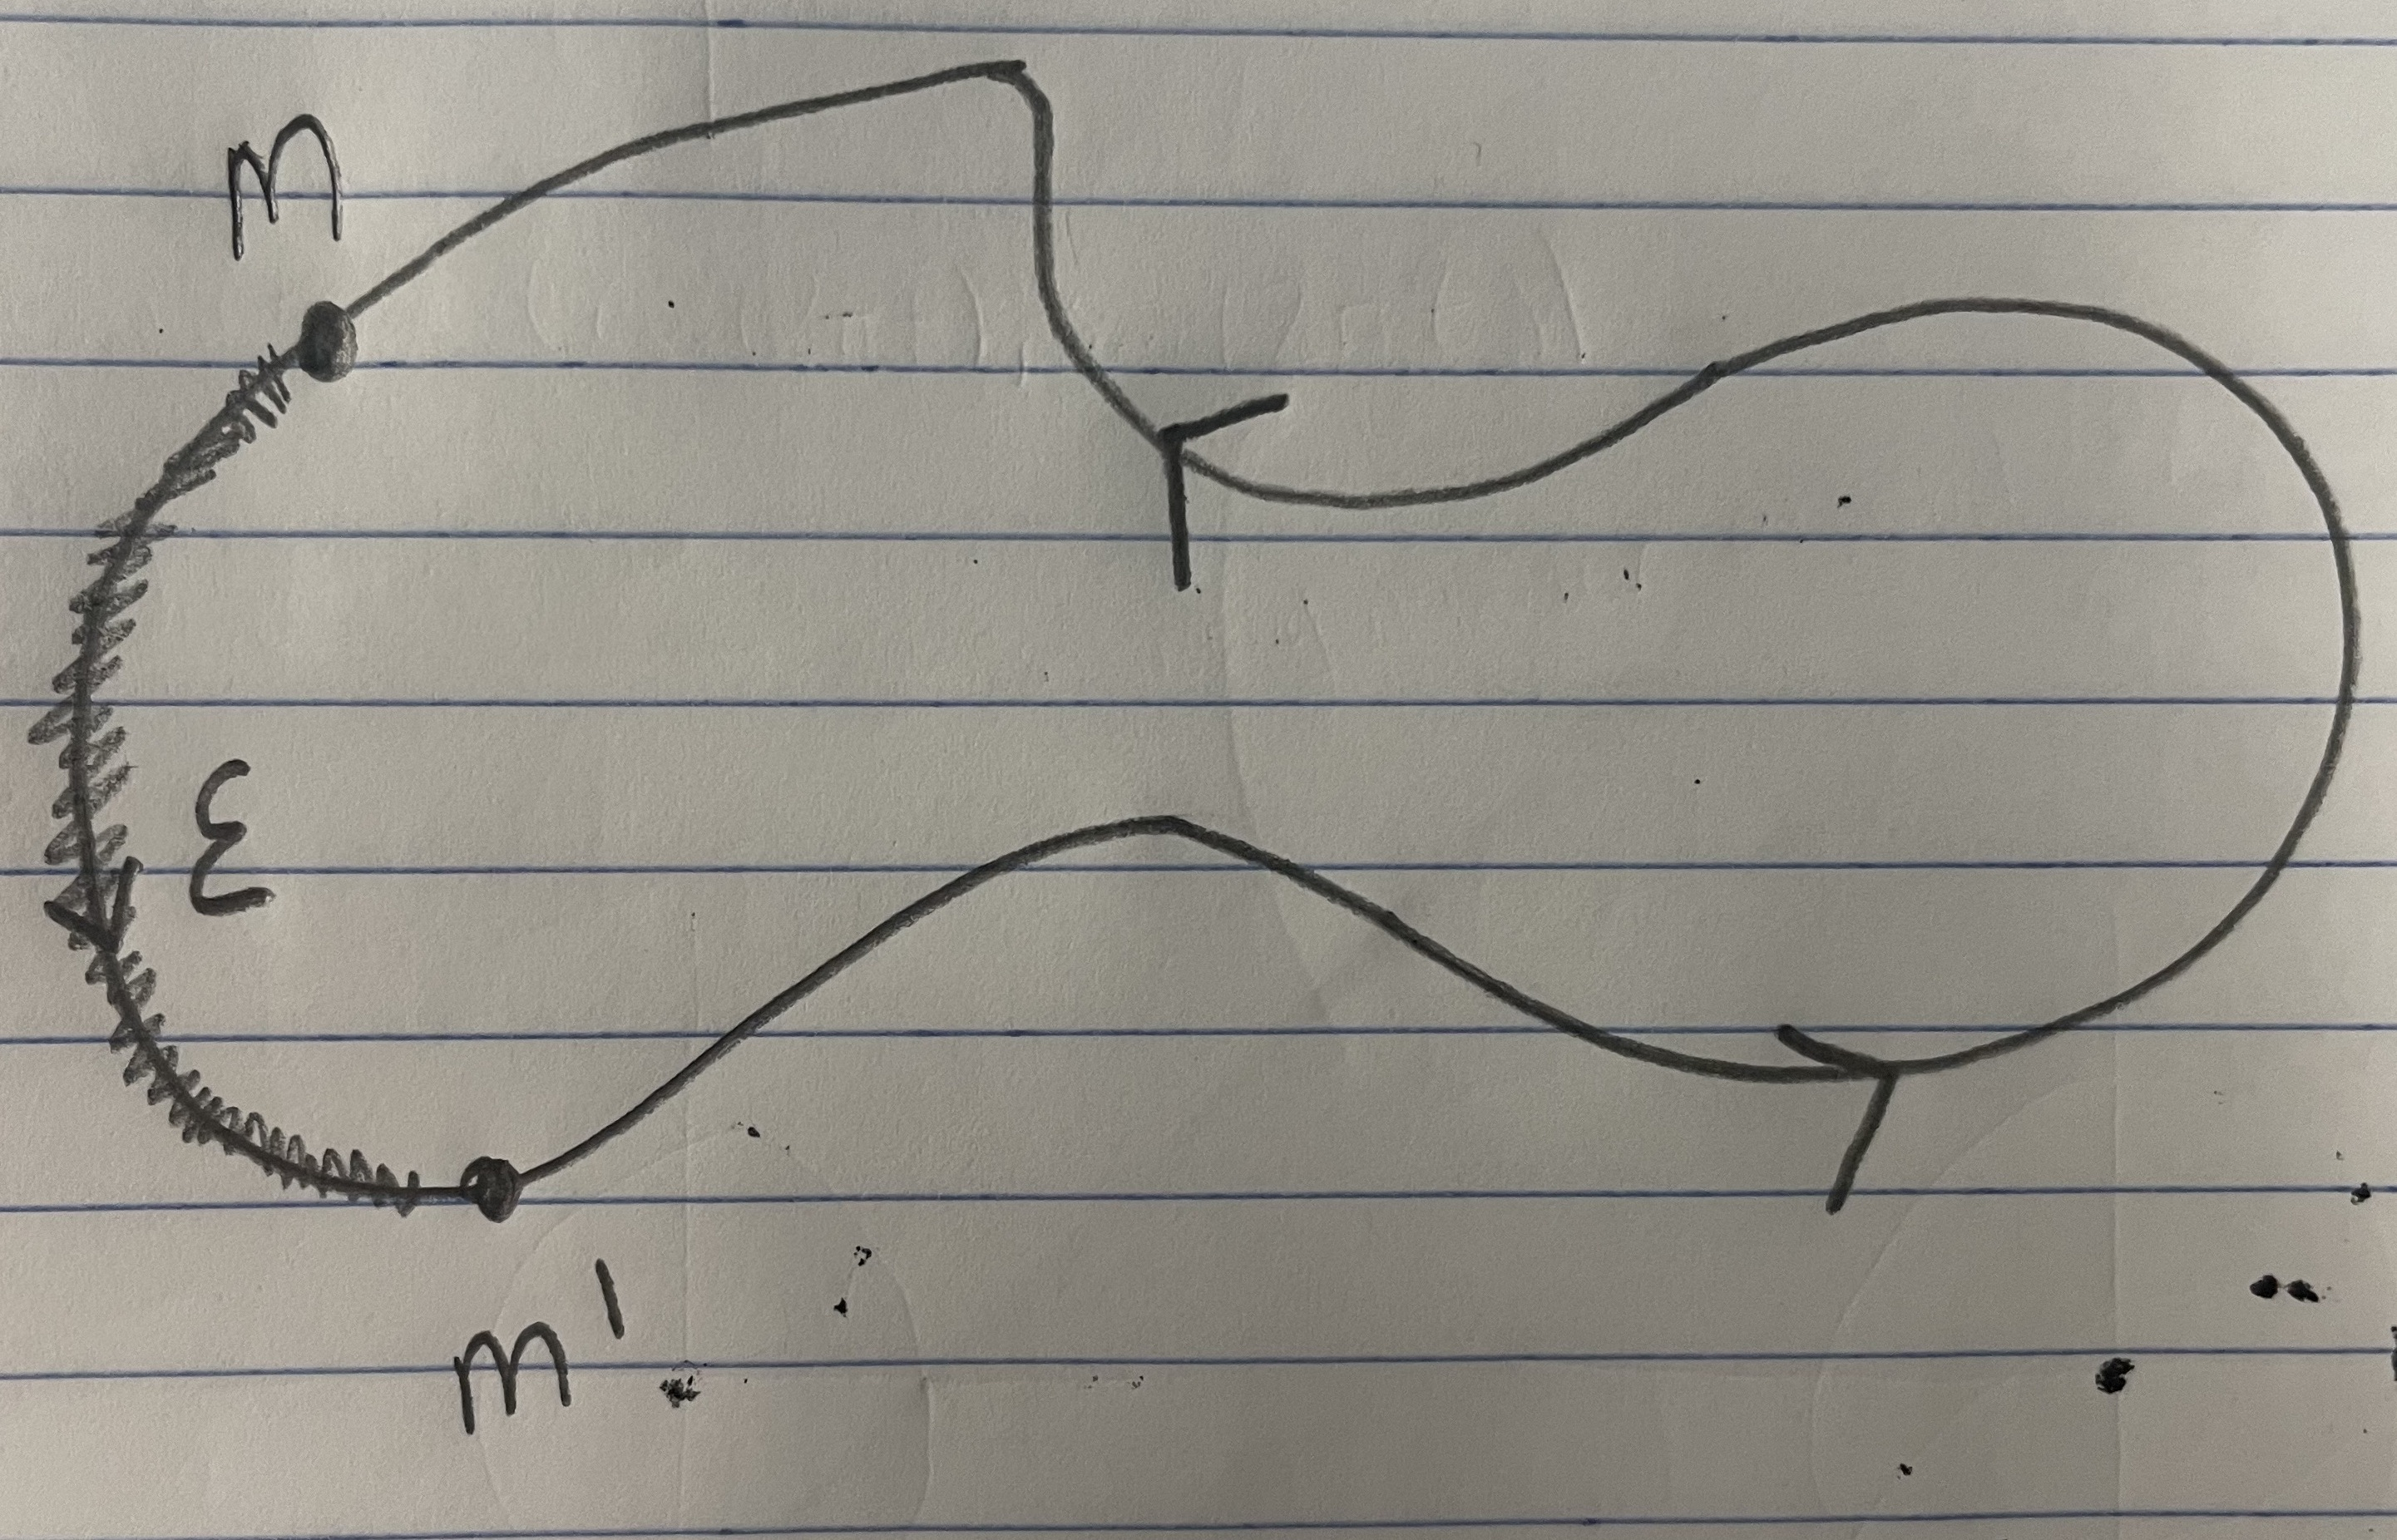
\includegraphics[scale=0.04]{conjugacy}
\caption{Illustration of why changing basepoints behaves as conjugation on loops .}
\label{conjugacy}
\end{center}
\end{figure}
\end{rem}

We can now use the fundamental group to analyse defects in ordered media. The first major insight is that loops in physical space yield loops in order space. Let $S\subset \bR$ be a finite set of defects and let $\phi: \bR^2 \backslash S \to M$ be a state. Given any loop $\alpha$ in $\bR^2\backslash S$ based at $b\not\in S$, postcomposing with $\phi$ gives a loop in $M$:

$$(\phi \circ \alpha): [0,1]\xrightarrow{\alpha} \bR^2 \backslash S \xrightarrow{\phi} M.$$

This loop has basepoint $(\phi \circ \alpha)(0)=(\phi\circ \alpha)(1)=\phi(b)$. The equivalence class of this loop up to basepoint preserving deformation is an element of $\pi_1(M,\phi(b))$. Given any state $\phi$ and given any loop $\alpha$ based at $b$, we denote the corresponding element of $\pi_1(M,\phi(b))$ by $\phi_*(\alpha)$, which we call the \textit{winding number of $\phi$ along $\alpha$}. This sort of winding number generalizes the standard notion of a winding number of a loop around a point discussed before.

Now, consider the system with $n$ defects arranged in a line. We can choose a basepoint $b$ above all of the defects. We add loops $\alpha_i$ based at $b$ for each $1\leq i \leq n$, each of which go directly around defect $i$ counterclockwise exactly once and do not go around any other defects. This setup is depicted in figure \ref{classical-setup}.

\begin{figure}
\begin{center}
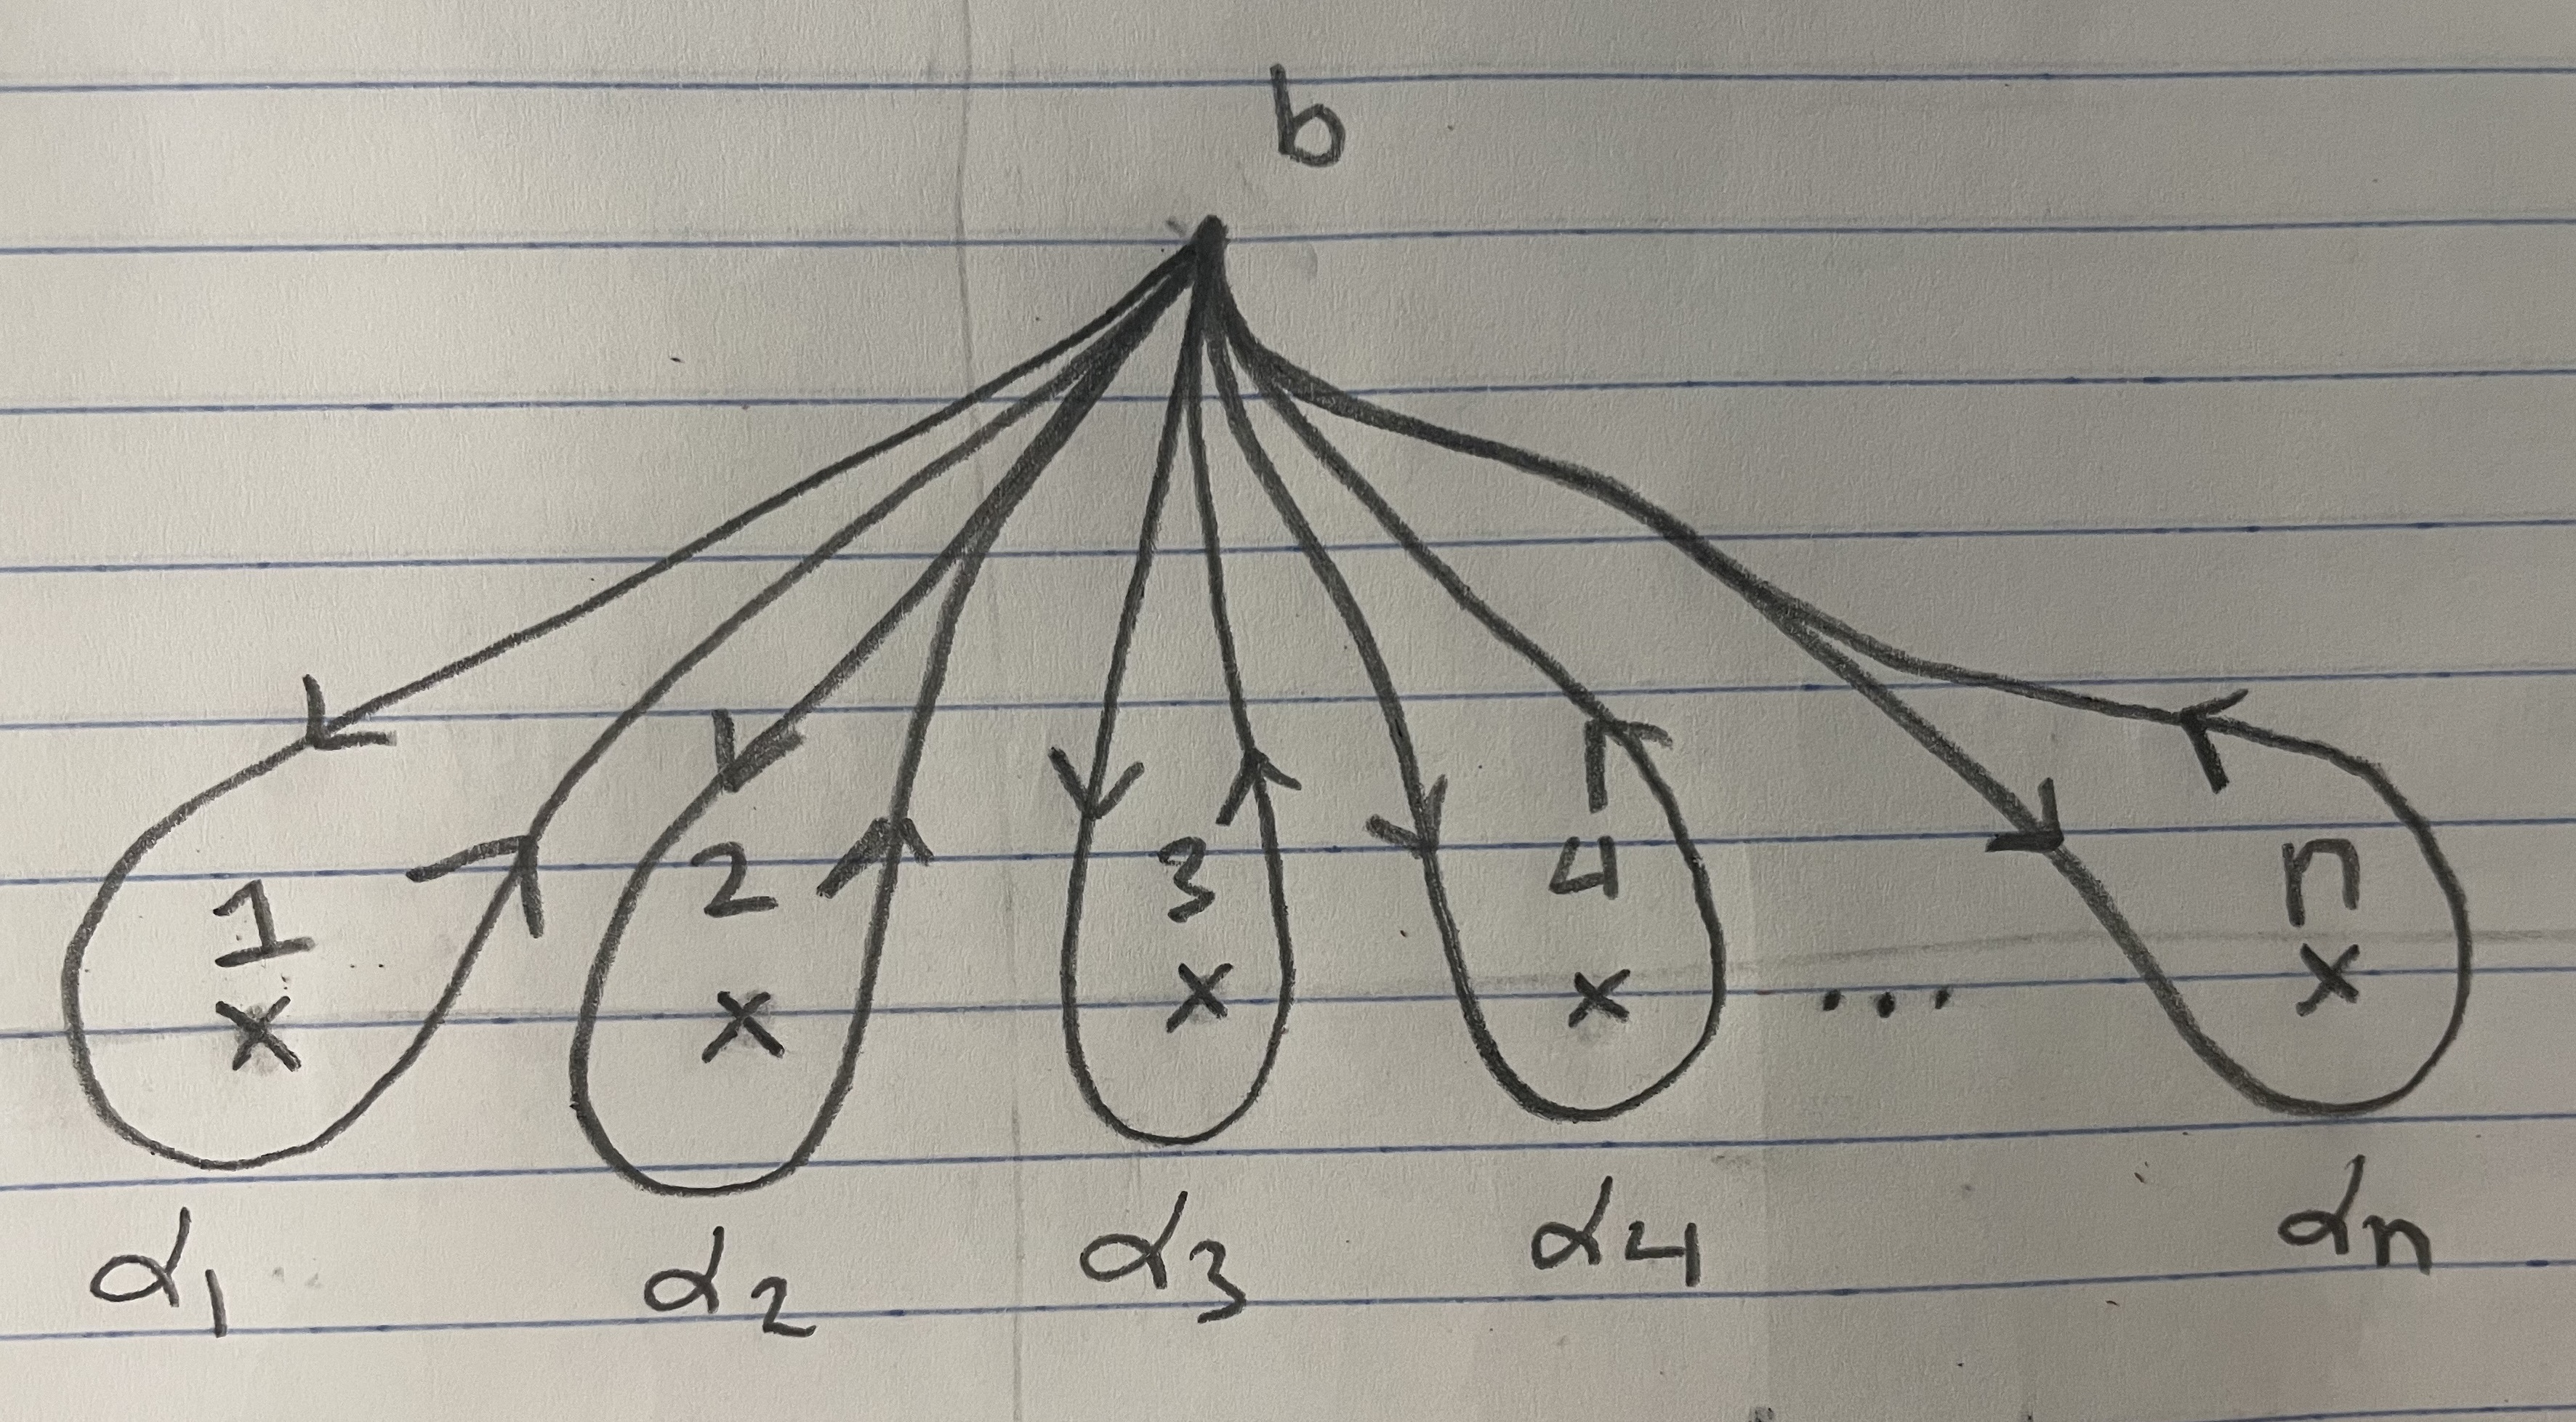
\includegraphics[scale=0.04]{classical-setup}
\caption{Defects arranged in a line with distinguished counterclockwise loops around each defect.}
\label{classical-setup}
\end{center}
\end{figure}

Given any ordered media state $\phi$ on this system, we can take the winding numbers $\phi_*(\alpha_i)\in \pi_1(M,\phi(b))$ of each loop $\alpha_i$. Applying a defect-fixed deformation could change the values $(\phi_*(\alpha_i))_{i=1}^n$ by a simultaneous conjugation on each component, because the defect-fixed deformation could change the value $\phi(b)$ assigned to the basepoint. Up to this global conjugation, however, the values $(\phi_*(\alpha_i))_{i=1}^n$ give a complete characterization of the information in $\phi$ which is invariant under defect-fixed deformations.

We now consider the behavior of these winding numbers $\phi_*(\alpha_i)$ under defect-mobile deformation. A defect mobile homotopy will have the effect of moving the defects around each other. Suppose that we have winding numbers $\phi_*(\alpha_i)=g_i\in \pi_1(M,\phi(b))$ for each $1\leq i\leq n$. Let $\tilde{\phi}$ be a state which is obtained by performing a defect-mobile deformation which moves defect $i$ above and around defect $i+1$, and which moves defect $i+1$ below and around defect $i$. This swap will result in a new state $\tilde{\phi}$ which is well-defined up to defect-fixed deformation. Denote the winding numbers $\tilde{\phi}_*(\alpha_i)=\tilde{g}_i\in \pi_1(M,\phi(b))$.

At every step along the defect-mobile deformation from $\phi$ to $\tilde{\phi}$ a loop can be drawn around defect $i$ connecting it to the basepoint $b$ so that these loops change continuously and never cross defect $i+1$. This means that the loop $\alpha_i$ at the beginning of the defect-mobile deformation is continuously deformed to the loop $\alpha_{i+1}$ after the deformation, and thus $\tilde{g}_{i+1}=g_i$. We observe additionally that the defect-mobile homotopy made no changes outside of a region localized around the defects $i$ and $i+1$ so the total winding number around defects $i$ and $i+1$ must be preserved. Thus, $\tilde{g}_i\tilde{g}_{i+1}=g_ig_{i+1}$. Combining these formulas, we conclude moving defect $i$ above and around defect $i+1$ has the following effect on winding numbers:

$$\tilde{g}_{i+1}=g_i,\,\,\,\,\,\,\,\,\,\,\,\,\,\, \tilde{g}_i=g_{i}g_{i+1}g_{i}^{-1}.$$ 

The above process is illustrated in figure \ref{braid-action}. If instead defect $i$ moves below and around defect $i+1$, the corresponding change in winding numbers is 

$$\tilde{g}_{i+1}=g_{i+1}^{-1}g_ig_{i+1},\,\,\,\,\,\,\,\,\,\,\,\,\,\, \tilde{g}_{i}=g_{i+1}.$$ 

\begin{figure}
\begin{center}
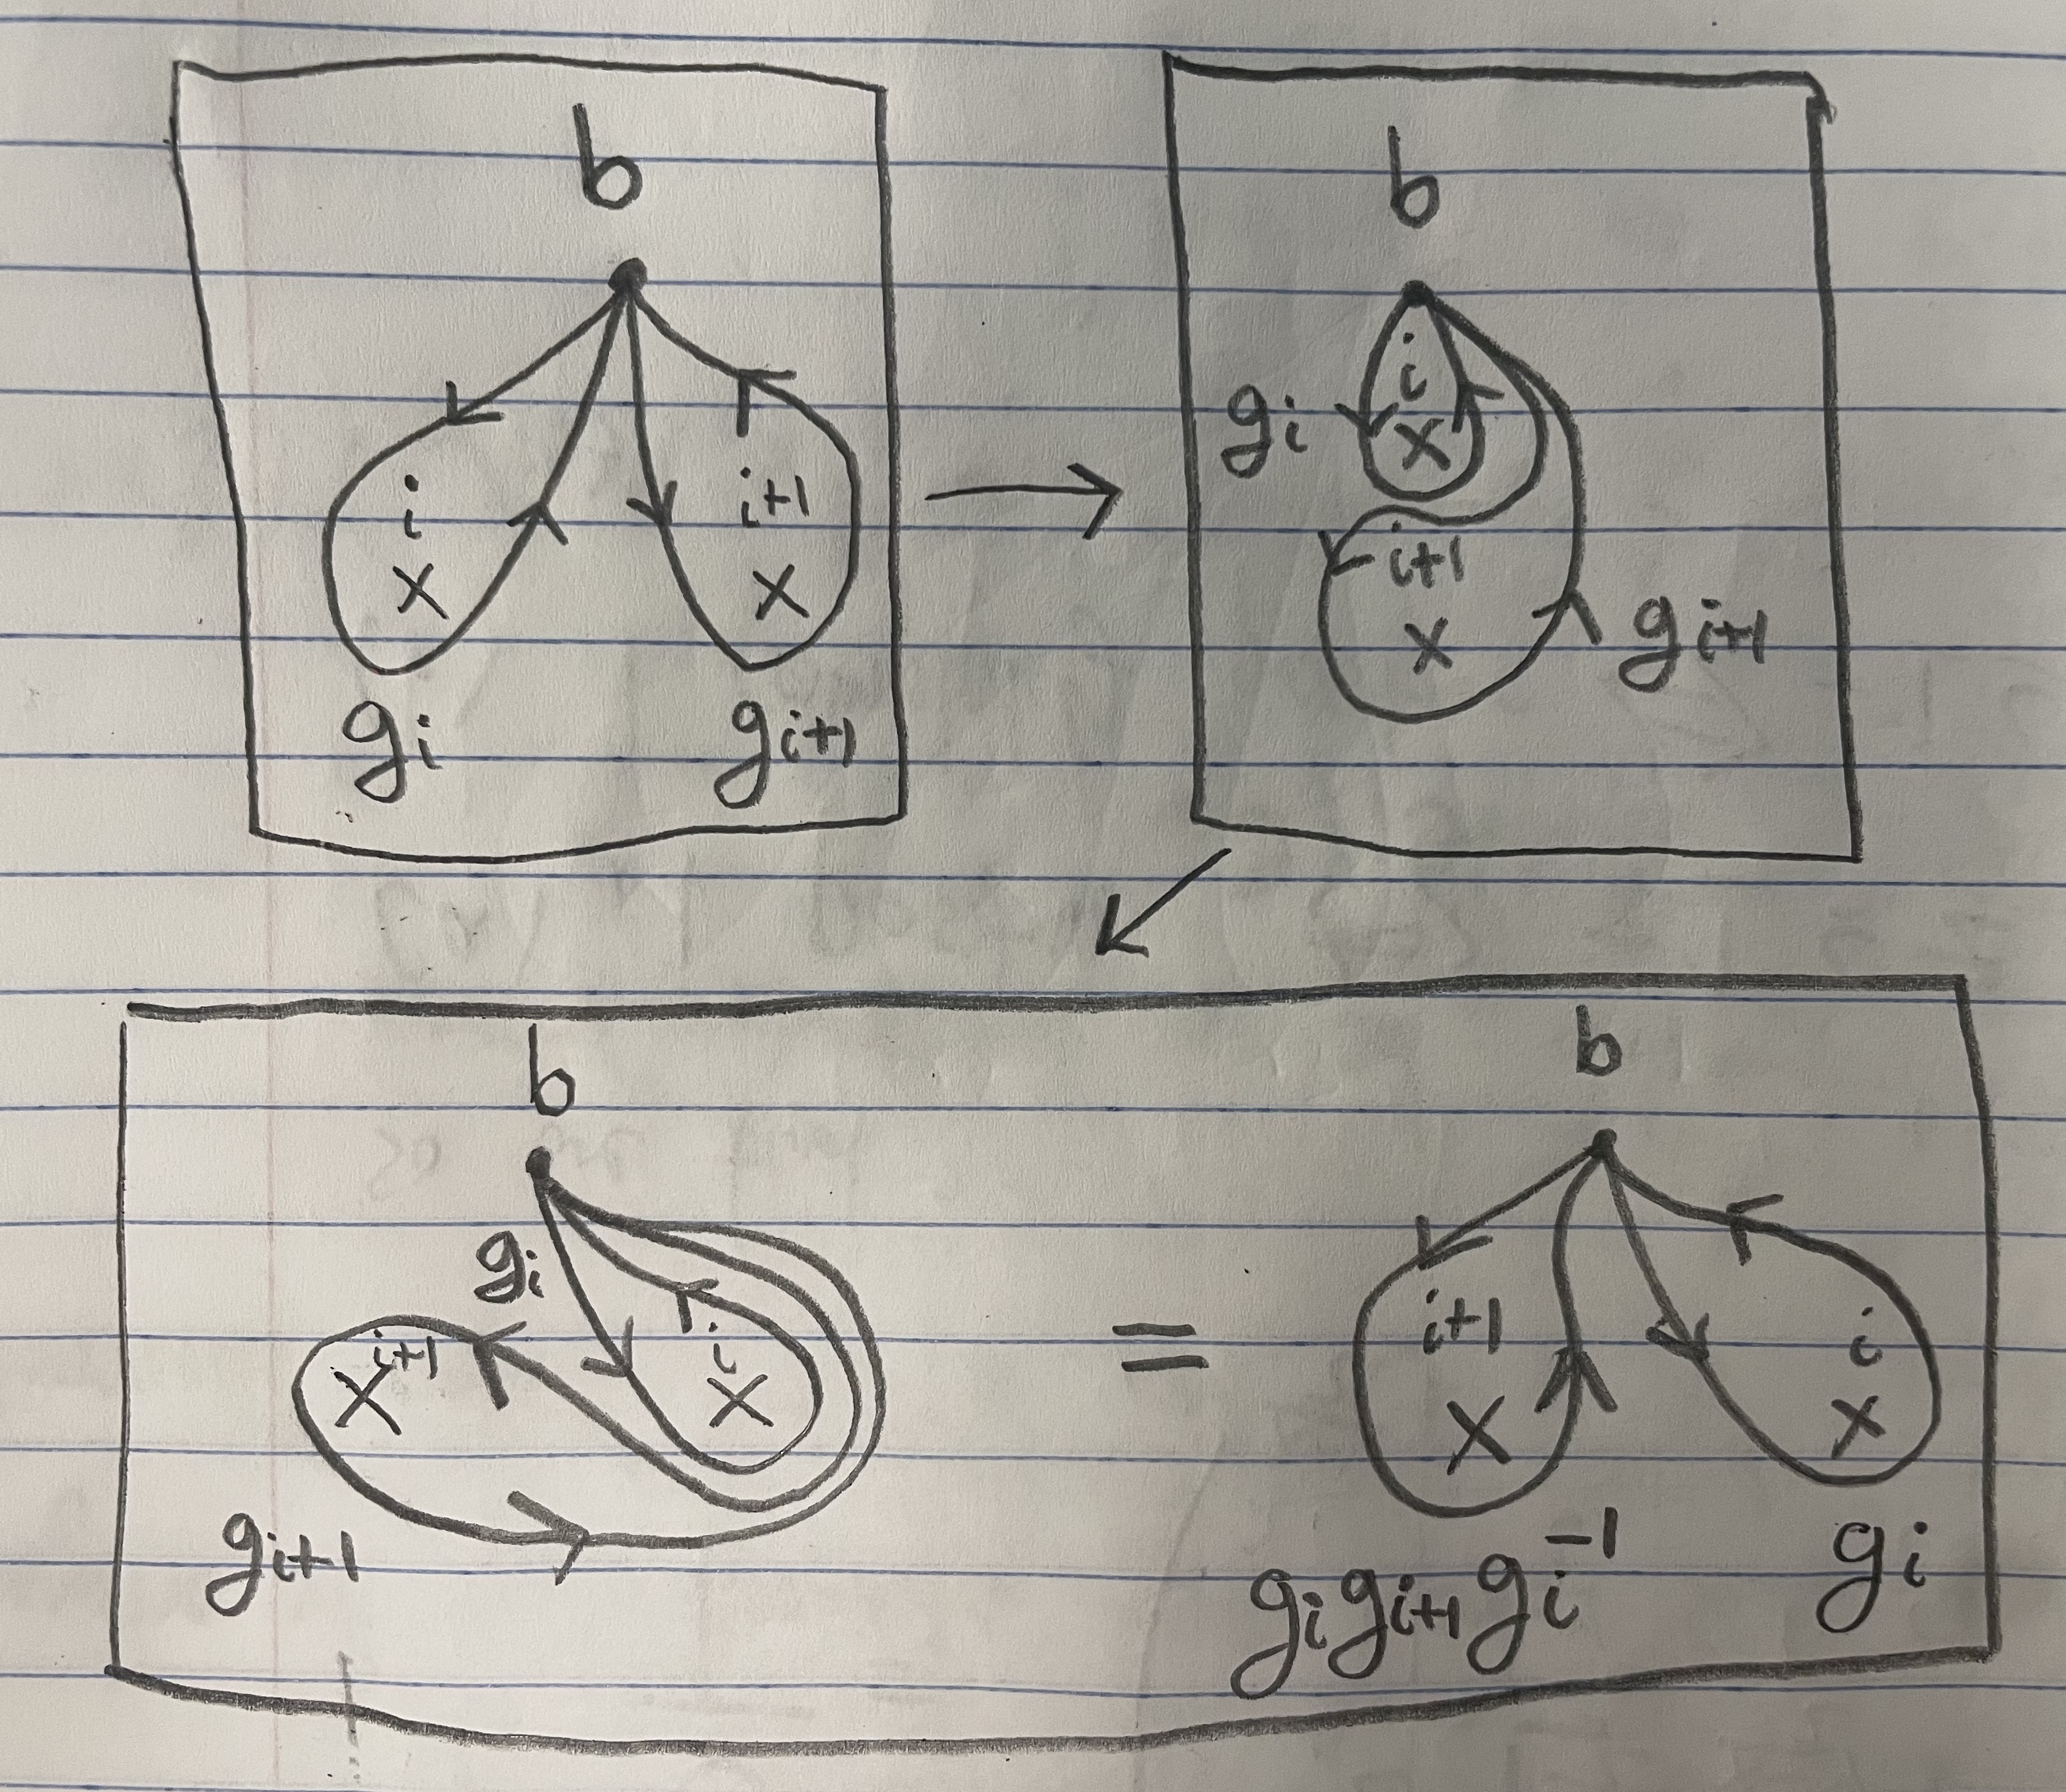
\includegraphics[scale=0.05]{braid-action}
\caption{Illustration of the effect of exchanging defects on winding numbers.}
\label{braid-action}
\end{center}
\end{figure}

The last ingredient we discuss are the locally measurable quantities in our system. Winding numbers are useful invariants of a state under defect-fixed deformation, but they are dependent on the choice of basepoint used. This means that the information encoded in the winding number is spread out over the whole region between the defect and the basepoint. This nonlocal nature makes it hard or impossible to measure in most reasonable physical implementations. A more readily measurable quantity is the winding number of a defect up to arbitrary deformation. That is, the conjugacy class in $\pi_1(M,\phi(b))$ associated to the defect. This conjugacy class can be computed using loops that are arbitararily close to the defect. Thus, it is a local quantity and can be effectively measured in physical implementations.

It is also desirabe to have a mechanism for reading out some non-local information about states in ordered media. A good way to do this is by fusing defects. Fusing defects is the process where nearby defects are brought close together until they act like a single defect. Fusion must preserve total winding number, and thus if two defects with winding number $g_1,g_2$ are fused then their resulting winding number is $g_1g_2$. The conjugacy classes of $g_1$ and $g_2$ are not enough to determine the conjugacy class of $g_1g_2$, and thus fusing two defects and then measuring the conjugacy class of their winding number gives access to more informaiton. In a sense, it gives access to the non-local information which was being stored between the two defects which are fused.

A sample measurement pattern is as follows.  Suppose that $\phi$ is a state with $n$ defects arranged in a line as before, and let us denote the winding numbers $\phi_*(\alpha_i)=g_i$. Local measurements give us access to the conjugacy classes of all of the elements $g_i$. By fusing the defects into the left-most defect one by one, we can access the conjugacy classes of $g_1$, $g_1g_2$,  $g_1g_2g_3$,... all the way up to $g_1g_2g_3...g_n$. In favorable situations these measurements can give a large amount of non-local information.

\subsubsection{Topological classical computation}
\label{topological-classical-computation}

We are now ready to describe the theory of topological classical computation. In the subsection \ref{the-fundamental-group}, we showed how all the topological information about defects in ordered media is controlled by the fundamental group $G=\pi_1(M,m)$ of the order space $M$ relative to some basepoint $m\in M$. This is the heart of the algebraic theory of topological computing. Even though our physical model is complicated, most information theoretic properties can understrood by analysing the algebraic structure $G$. In fact, we can now formulate our discussion of topological classical computation in a way which does not make reference to the order space at all. We will choose an abstract group $G$ and make a computer using it. This gives the following schematic for our discussion:

\begin{equation*}
\tikzfig{mathematical-outline-classical}
\end{equation*}

That is, our construction of topological classical computers from ordered media {\em factors through} group theory. This schematic is similar to the overall structure of this book, which we said before is summarized by this diagram:

\begin{equation*}
\tikzfig{mathematical-outline}
\end{equation*}

\begin{rem}
Just like how groups are the structures which control the algebraic theory of ordered media, modular categories are the structure which control the algebraic theory topologically ordered systems. In fact, this analogy this analogy can be made precise. The idea is that ordered media can be {\em quantized}, turning it from a classical to a quantum system. This quantized version of ordered media is known as {\em discrete gauge theory}. Quantization is a subtle procedure, which we will discuss in section \ref{topological-quantum-order}. When the group $G=\pi_1(M,m)$ is infinite the quantization procedure goes wrong, because there are divergences in the formulas. Hence, quantization of ordered media only works for finite groups. The algebraic structure controlling the quantized version of ordered media based on a finite group $G$ is $\fD(G)$, where $\fD(G)$ is a modular category constructed using the finite group $G$. So, in a real sense, modular categories can be seen as vast quantum generalizations of finite groups. This is often a useful perspective to take.
\end{rem}

We now set up topological classical computing with ordered media, along the same lines as our abstract setup in subsection \ref{principles-of-tqi}. Our system consists of $n$ defects on a straight line. These defects are labeled with group elements $g_i\in G$, for $1\leq i \leq n$. These labels correspond to winding numbers around loops:

\begin{figure}
\begin{center}
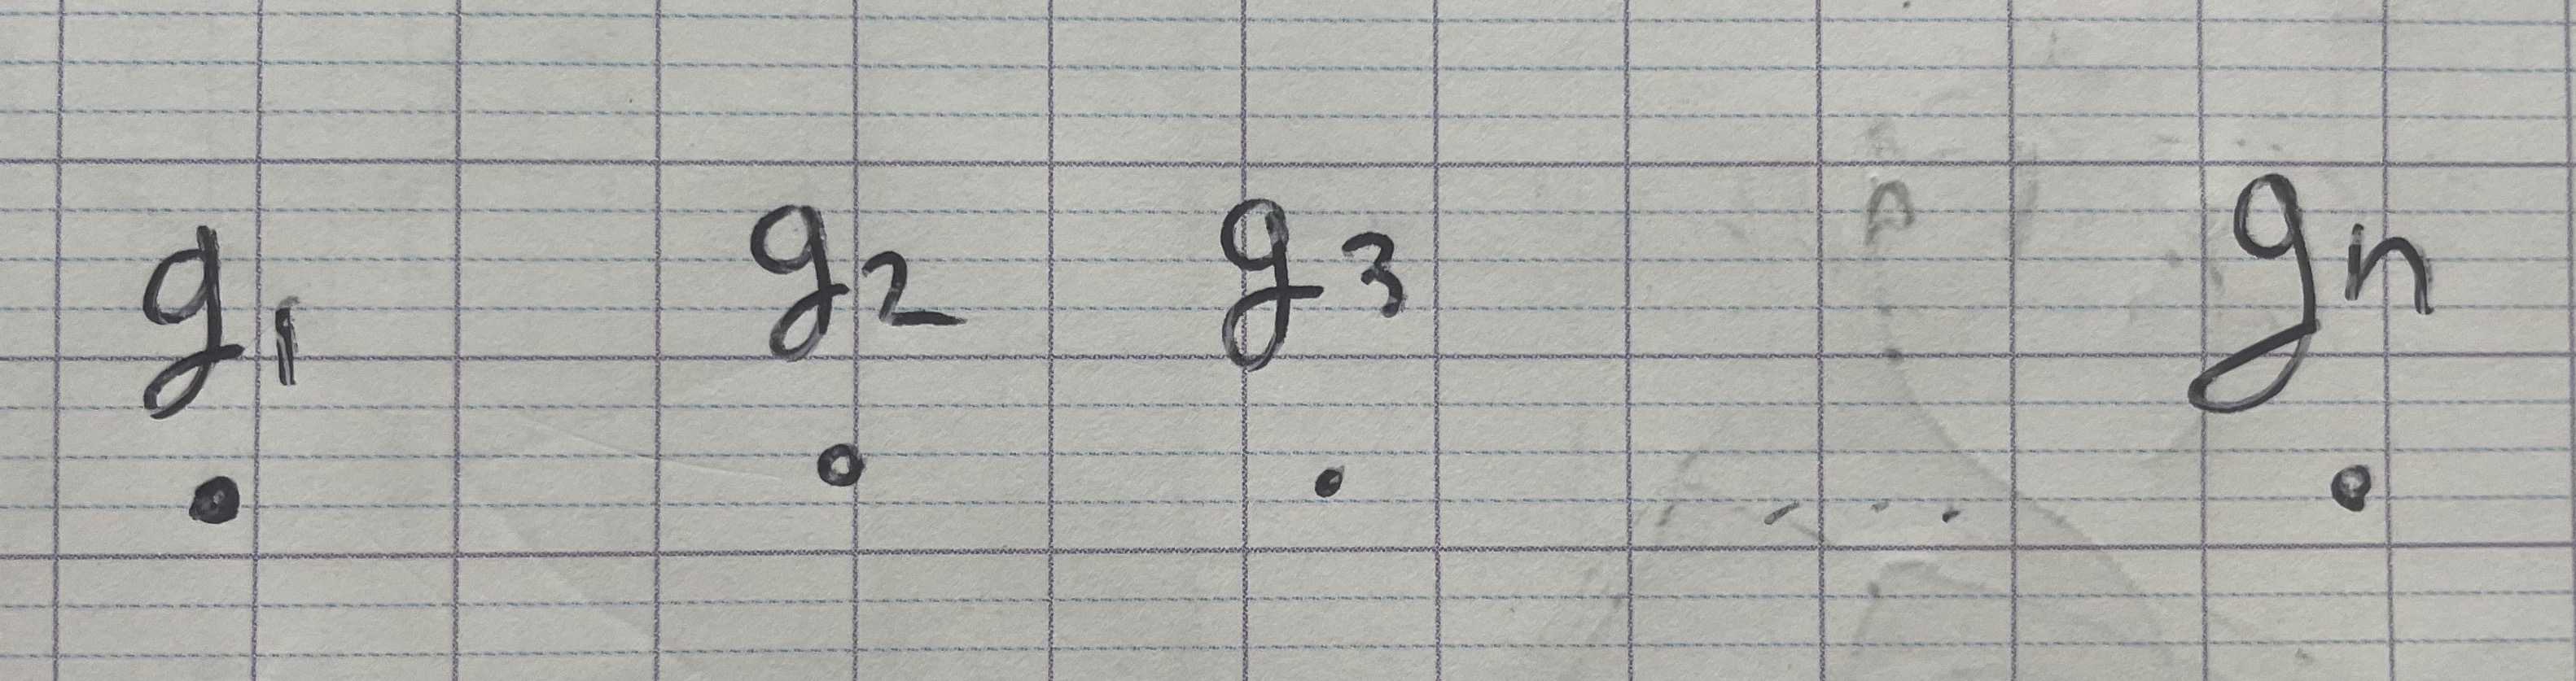
\includegraphics[scale=0.05]{winding-numbers}
\label{winding-numbers}
\end{center}
\end{figure}

Braiding $g_i$ under and around $g_{i+1}$ amounts to replacing $g_i$ with $g_{i+1}$, and replacing $g_{i+1}$ with $g_{i+1}^{-1}g_i g_{i+1}$. Fusing the defects $g_{i}$ and $g_{i+1}$ amounts to replacing them with a single defect labeled $g_{i}g_{i+1}$. The \textit{type} of a defect is the conjugacy class of its label in $G$. The types of the defects are local observables which can be measured by the experimenter.

\begin{figure}
\begin{center}
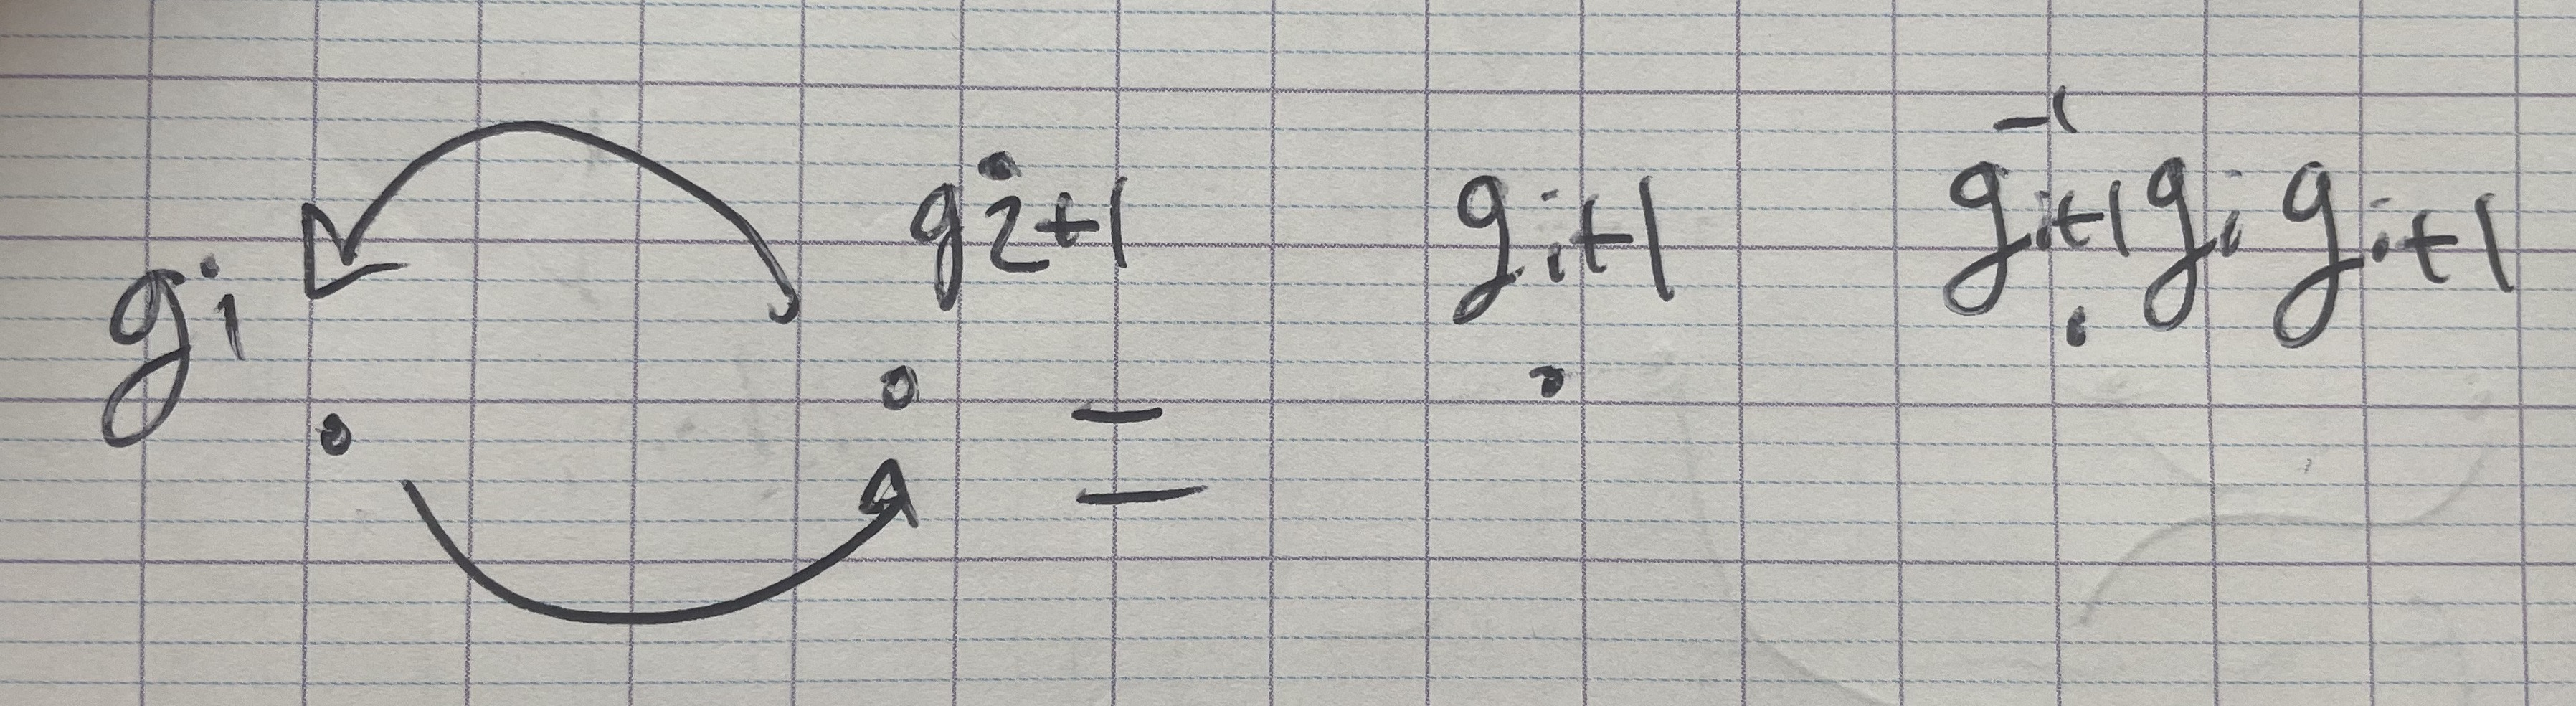
\includegraphics[scale=0.05]{braiding-rule}
\label{braiding-rule}
\end{center}
\end{figure}

\begin{figure}
\begin{center}
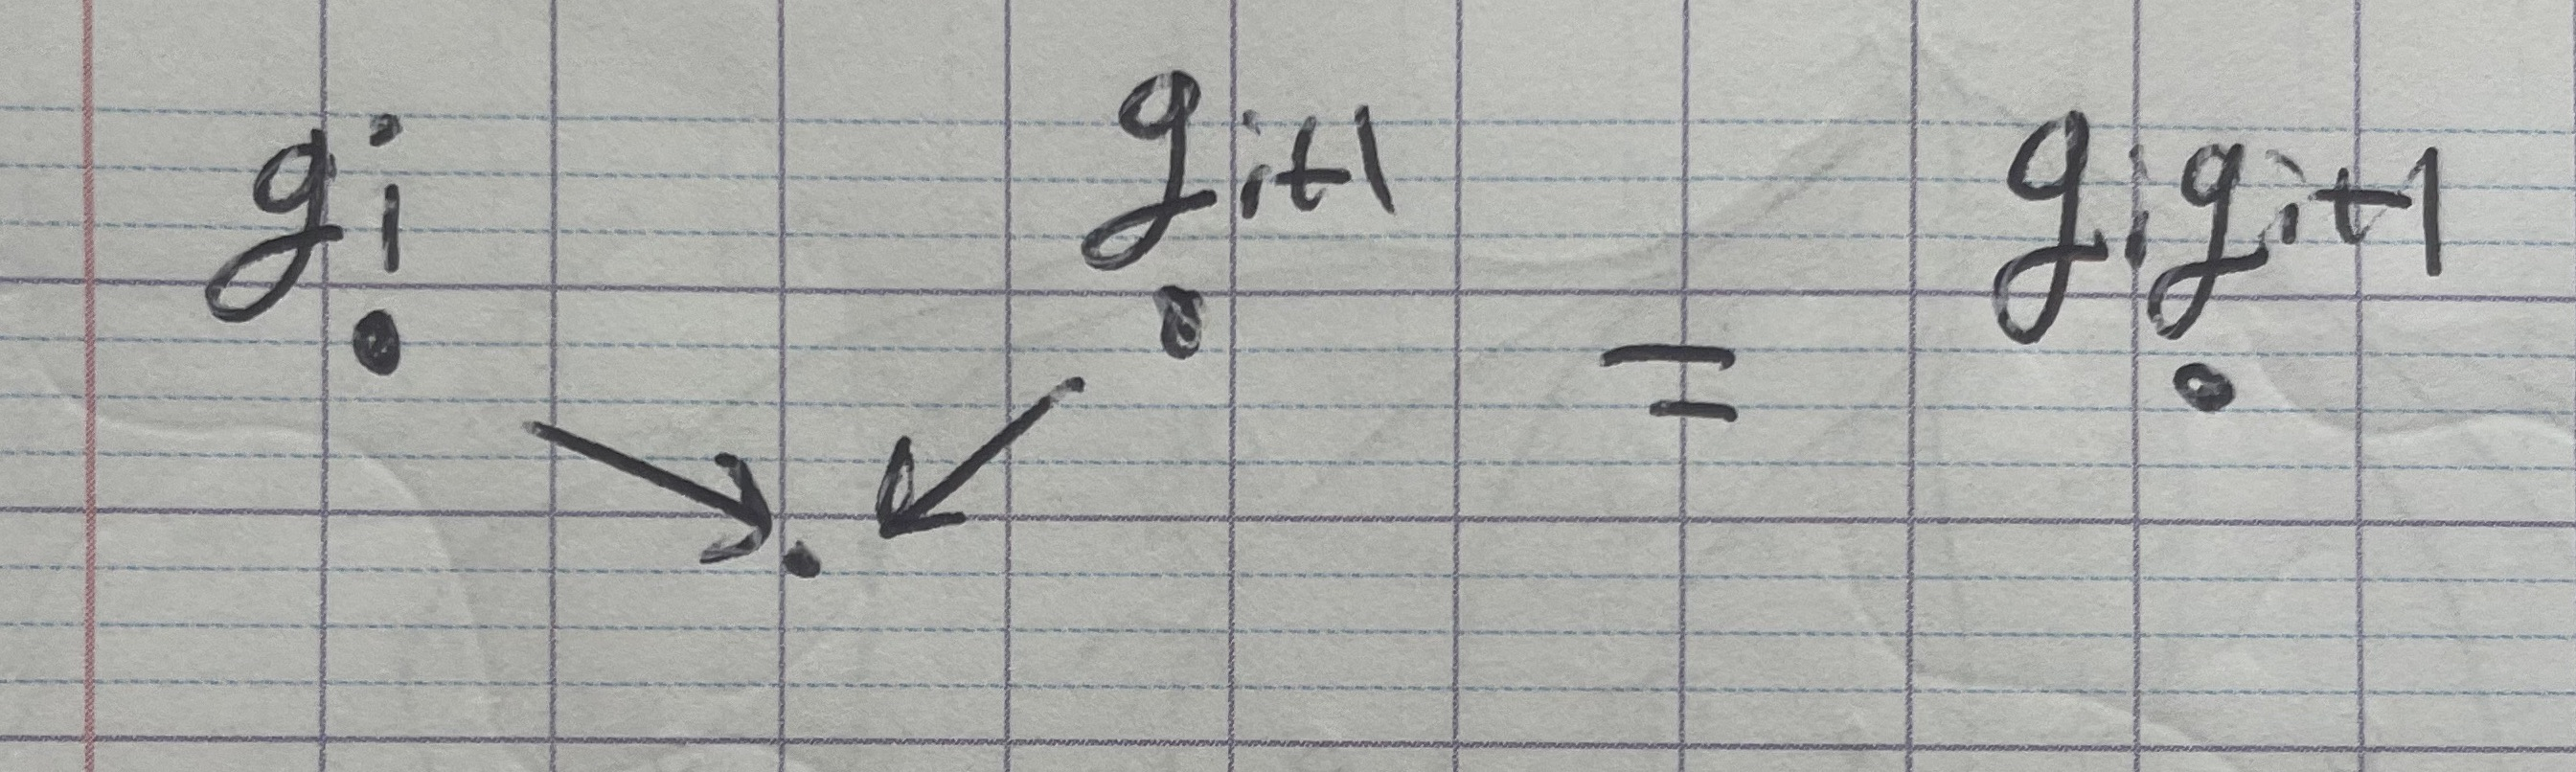
\includegraphics[scale=0.05]{fusion-rule}
\label{fusion-rule}
\end{center}
\end{figure}

Our previous discussion of braiding was heuristic, but we are now ready to put it on firm footing. We first try to capture our intuitive notion of braiding from before. Intutively, we consider a braiding operation to be some way of moving $n$ points arrangened on a line in $\bR^2$ around each so that the end position of each point is equal to the start position of some other point. For example, moving one point under and around another point is a braiding operation. Continuous deformations do not change the effect of braiding operations on topological information, so long as they do not change the initial or final positions of any of the points. Thus, for any integer $n\geq 1$ we define the \textit{braid group on $n$ stands}:

$$B_n=(\text{braiding operations on $n$ points})/(\substack{\text{endpoint-preserving} \\ \text{continuous deformations}}).$$

We call elements of $B_n$ {\em braids}. We call the trajectories of the individual points through time \textit{strands}. We can also define the {\em pure braid group on $n$ strands} $P_n$ to be the subset of braids such that the final position of every point is equal to its initial position. Elements of $P_n$ are called {\em pure braids}.

To facilitate our discussion of braids, we use a graphical notation which tracks the trajectories of the points through time. For instance, the braiding operation in the two-strand braid group$B_2$ which moves one point above and around the other point is represented through the following diagram:

\begin{figure}[h]
\begin{center}
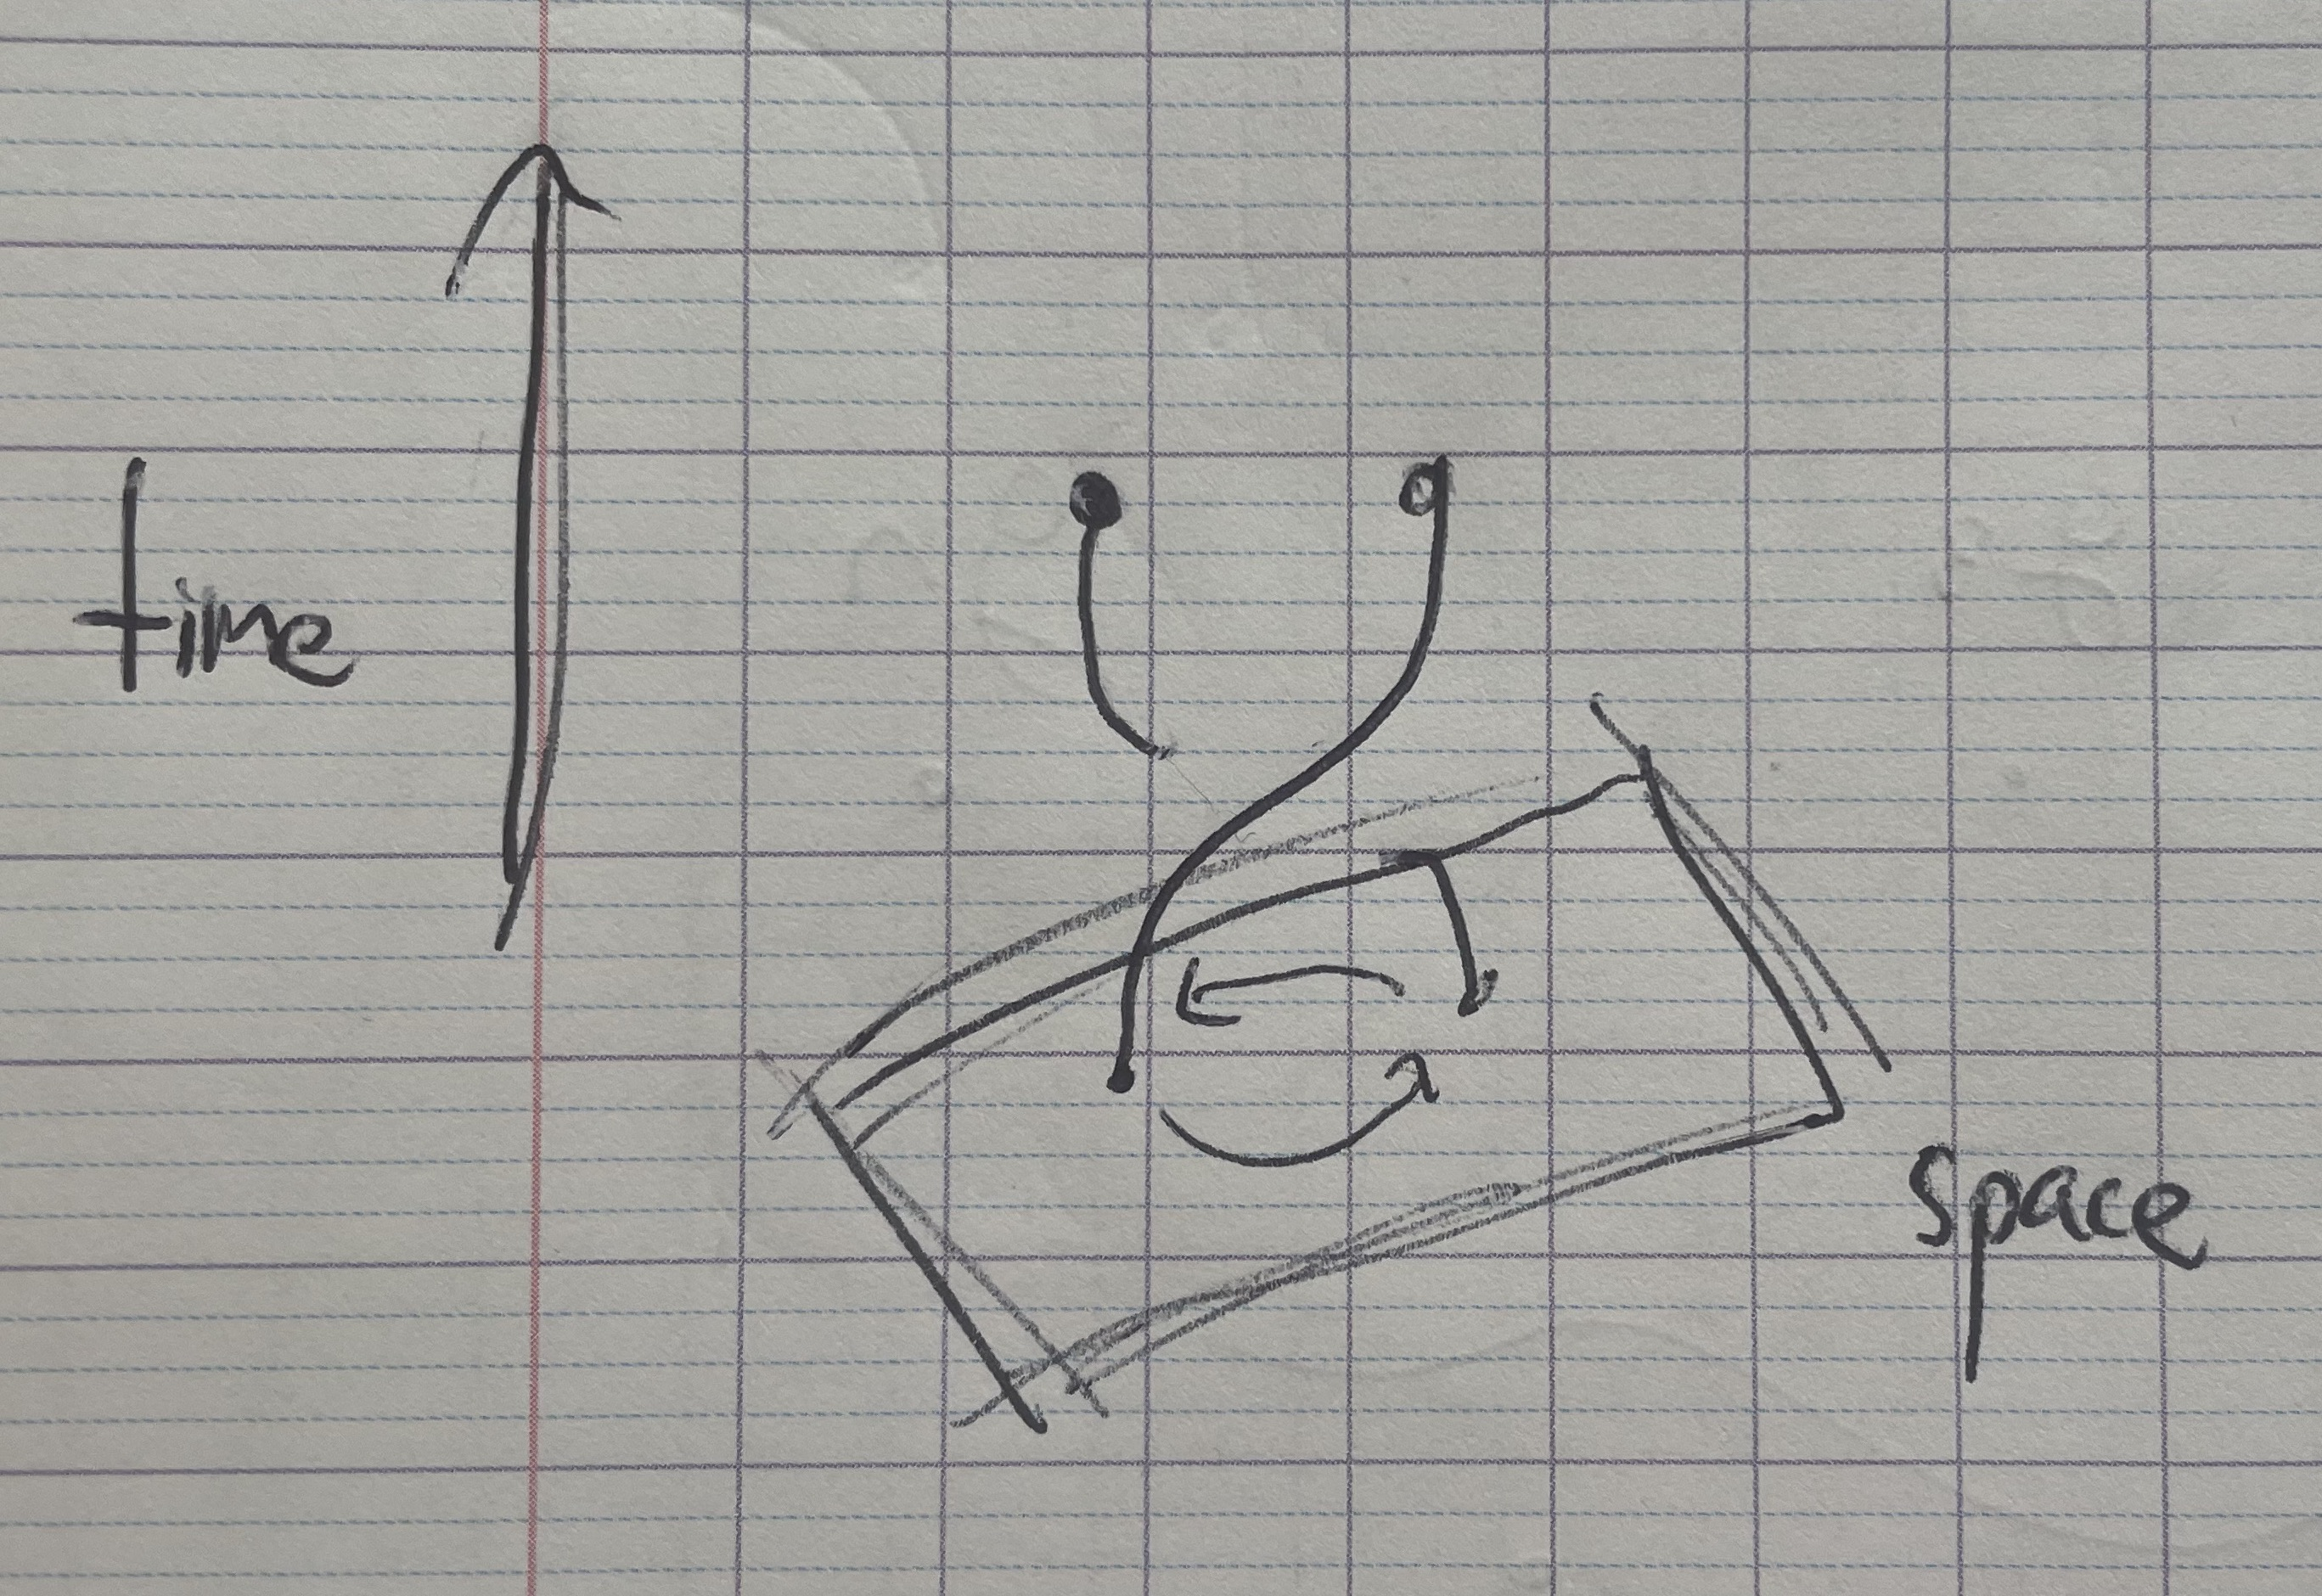
\includegraphics[scale=0.05]{braiding-diagramatic}
\label{braiding-diagramatic}
\end{center}
\end{figure}

\begin{figure}
\begin{center}
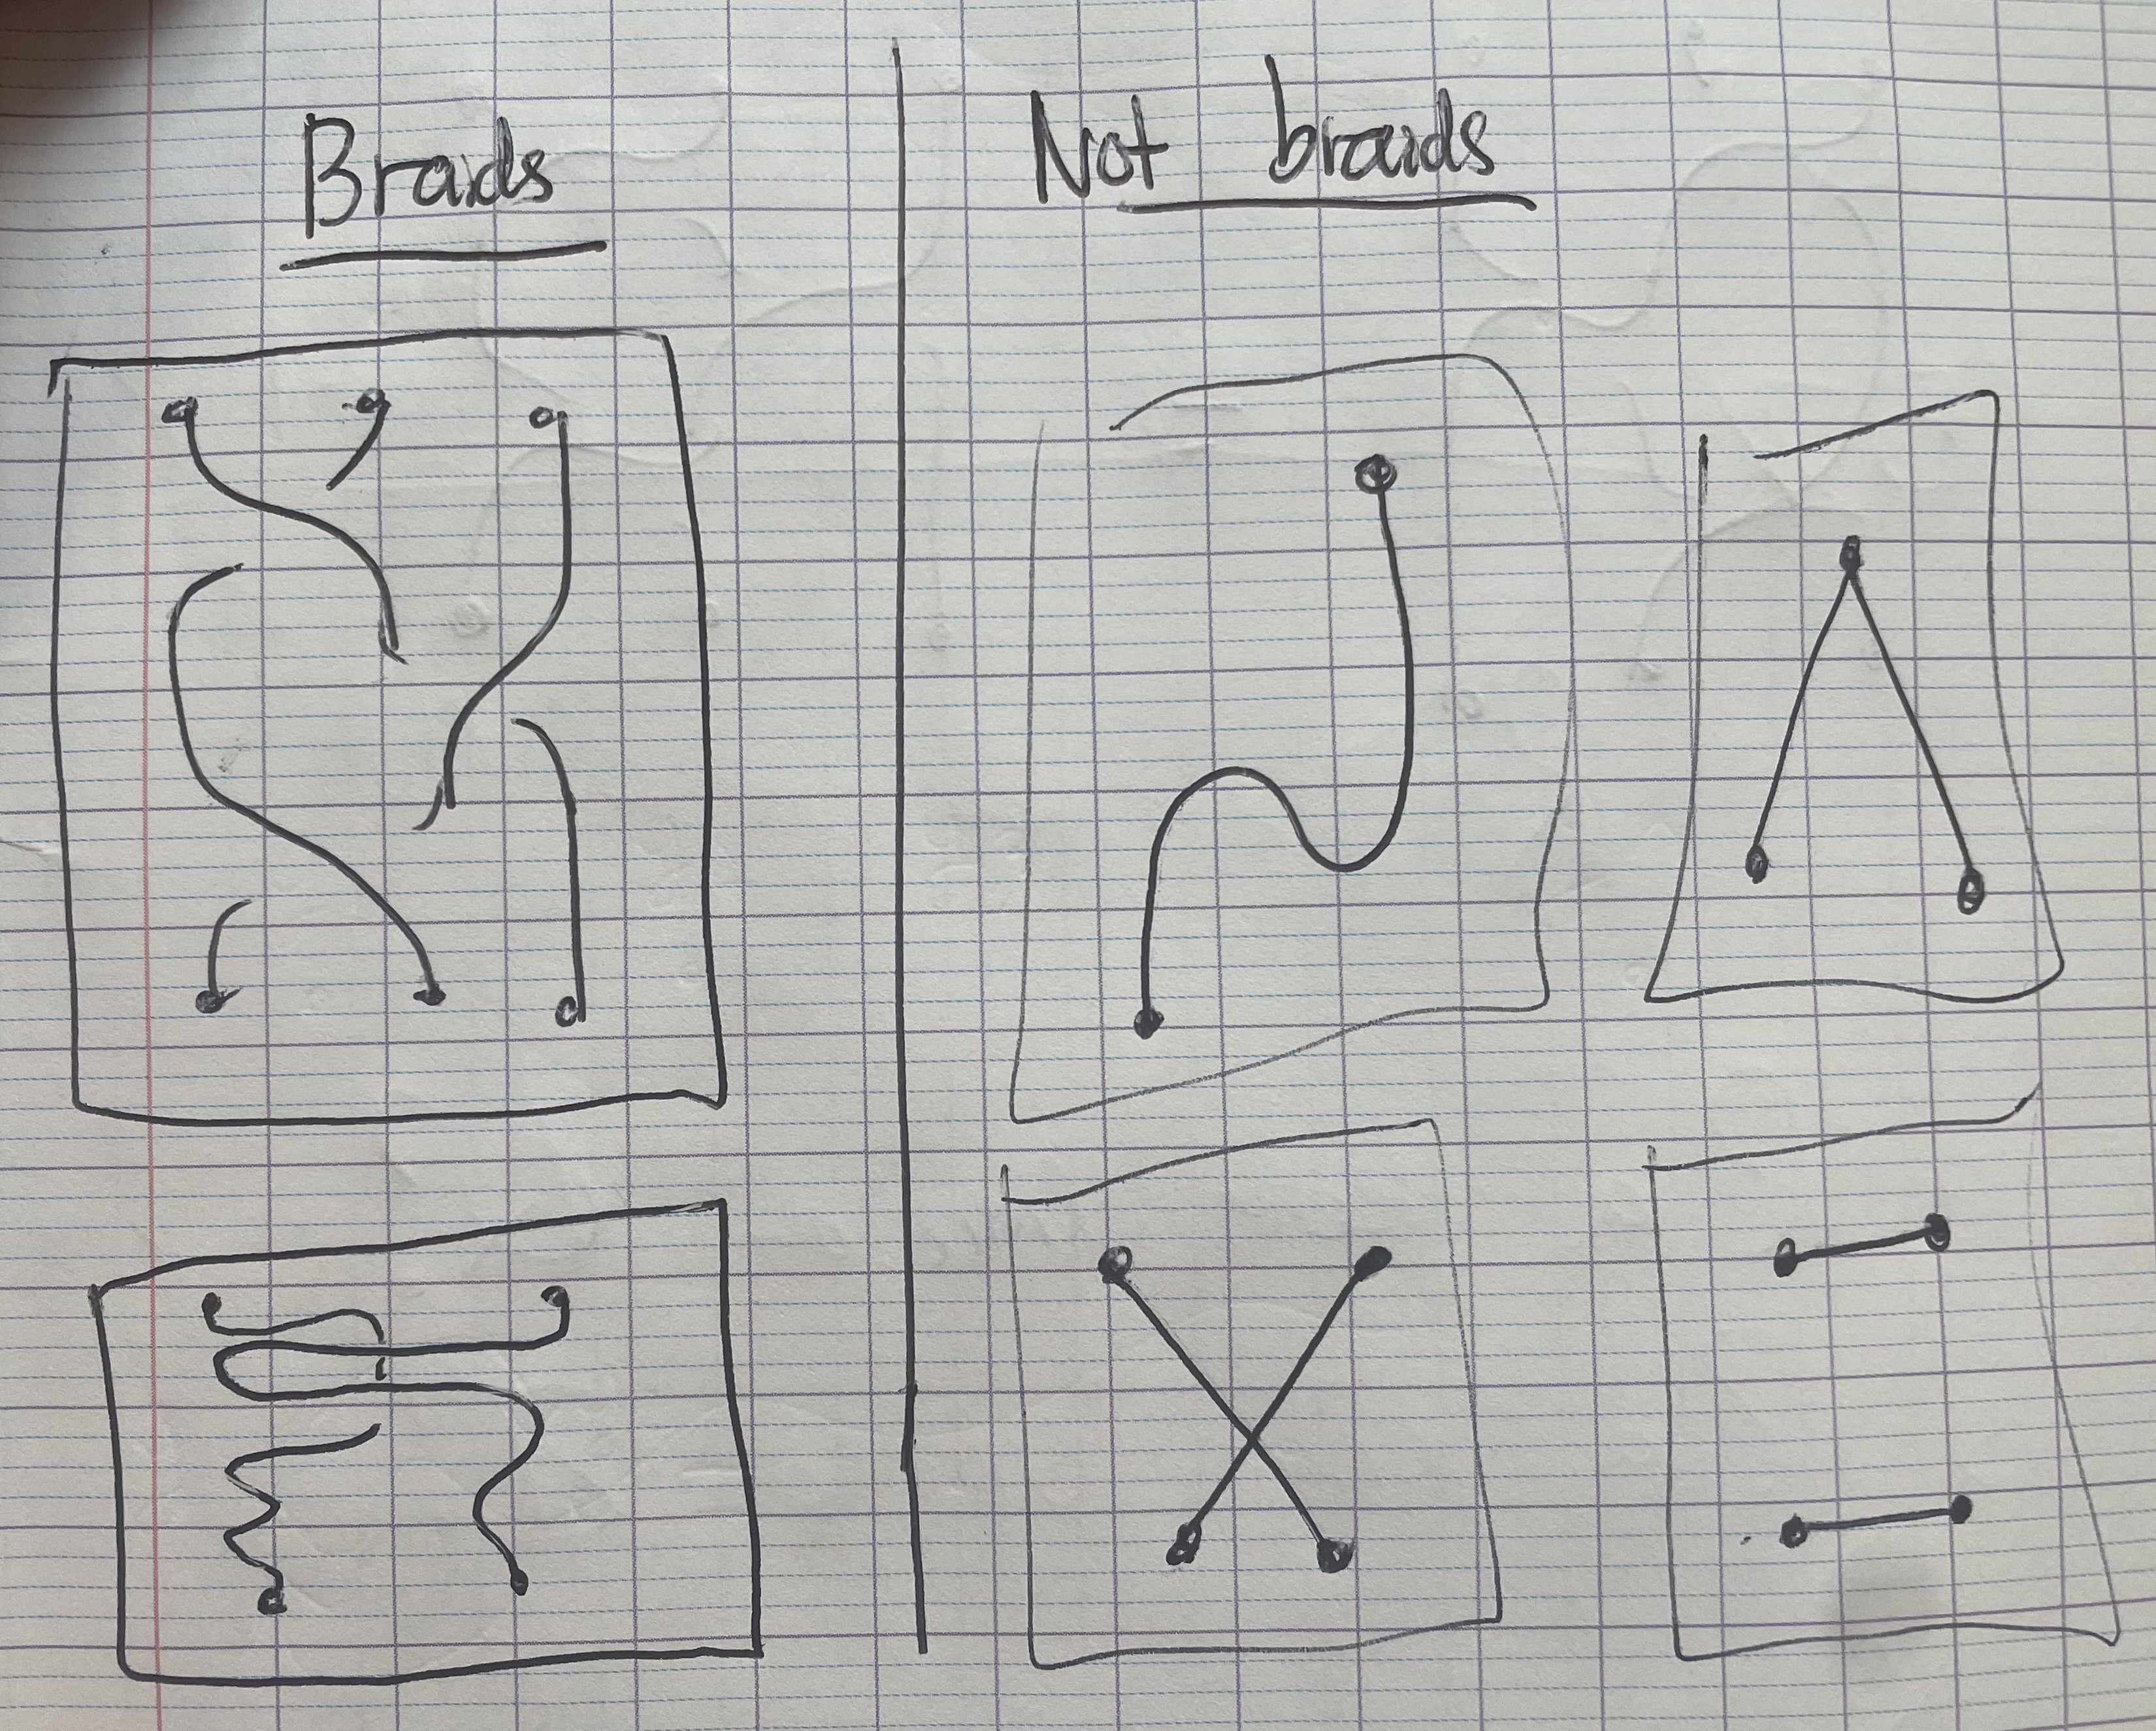
\includegraphics[scale=0.05]{braiding-examples}
\label{braiding-examples}
\end{center}
\end{figure}

The braid group is called a group because it has a natural group structure on it induced by composition. Given any two braiding operations on $n$ points, composing them will give another braiding operation!  Composition is well-defined on equivalence classes under continuous deformation, and thus it gives a well-defined group structure. The unit element for this group structure is the equivalence class of the braiding operation which does not move the points at all, and the inverse of a braid comes from taking a braiding operation and then reversing its direction in time. This turns $B_n$ into a group, and $P_n$ into a normal subgroup.

The key insight in putting the braid group on a rigorous algberaic footing is to observe that every braid can be obtained by repeatedly composing nearest-neighbor swaps between points. This is done by chopping it its spacetime diagram into slices which each contain an individual swap, as shown below:

\begin{figure}[h]
\begin{center}
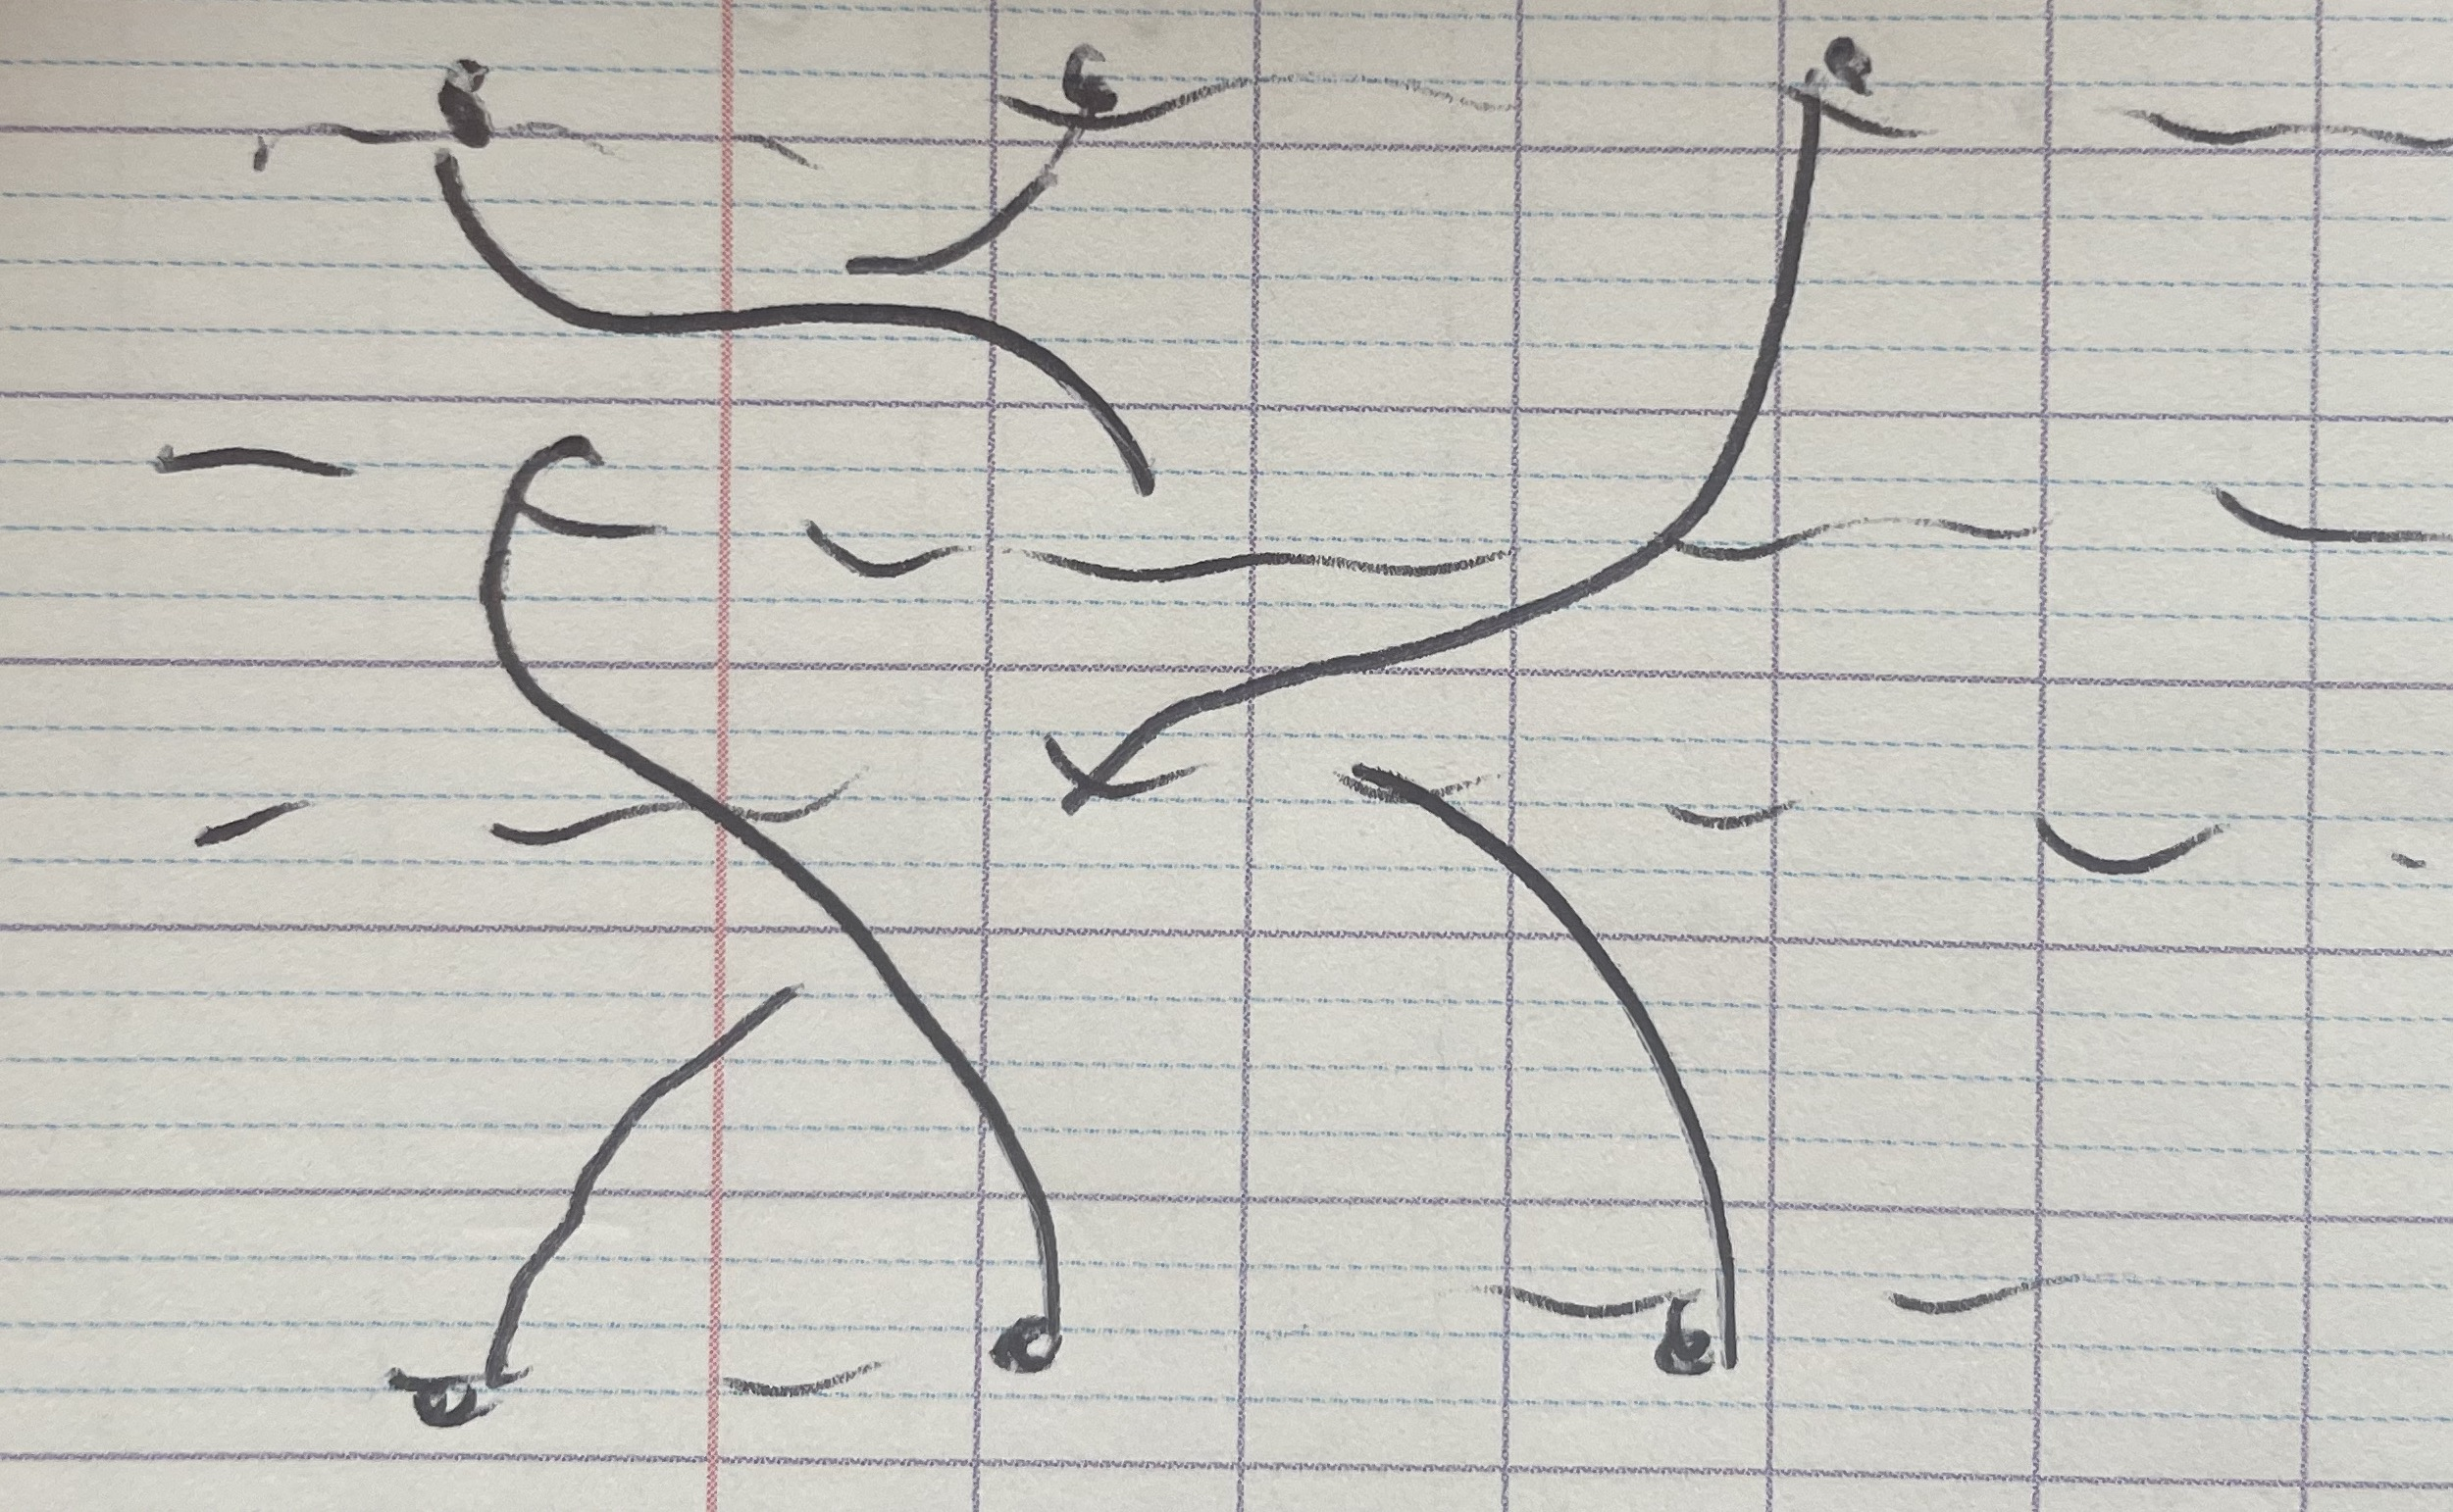
\includegraphics[scale=0.05]{braiding-decomposition}
\label{braiding-decomposition}
\end{center}
\end{figure}


If two crossings happen at the same time and hence cannot be seperated by chopping, then the braid is first deformed so that the crossings happen at seperate times and then the braid is chopped. This decomposition observation has a quite concrete implication for the group theory of $B_n$. For every $1\leq i\leq n-1$, define the braid $\sigma_{i}$ to be the equivalence class of the braiding operation which moves point $i$ above and around point $i+1$. By chopping braidins into indivudal swaps, we conclude that $B_n$ is generated as a group by the braids $\sigma_i$, $1\leq i\leq n-1$.

These generators $\sigma_i$, $1\leq i\leq n-1$, satisfy several relations in $B_n$. The obvious relations between them is that $\sigma_i$ commutes with $\sigma_j$ whenever $|i-j|\geq 2$. This is because in this case $\sigma_i$ and $\sigma_j$ act on different strands, and hence can be deformed past each other without issues. The subtle relation is what happens when $j=i+1$. In this case, we observe the following equality of braids:

\begin{figure}
\begin{center}
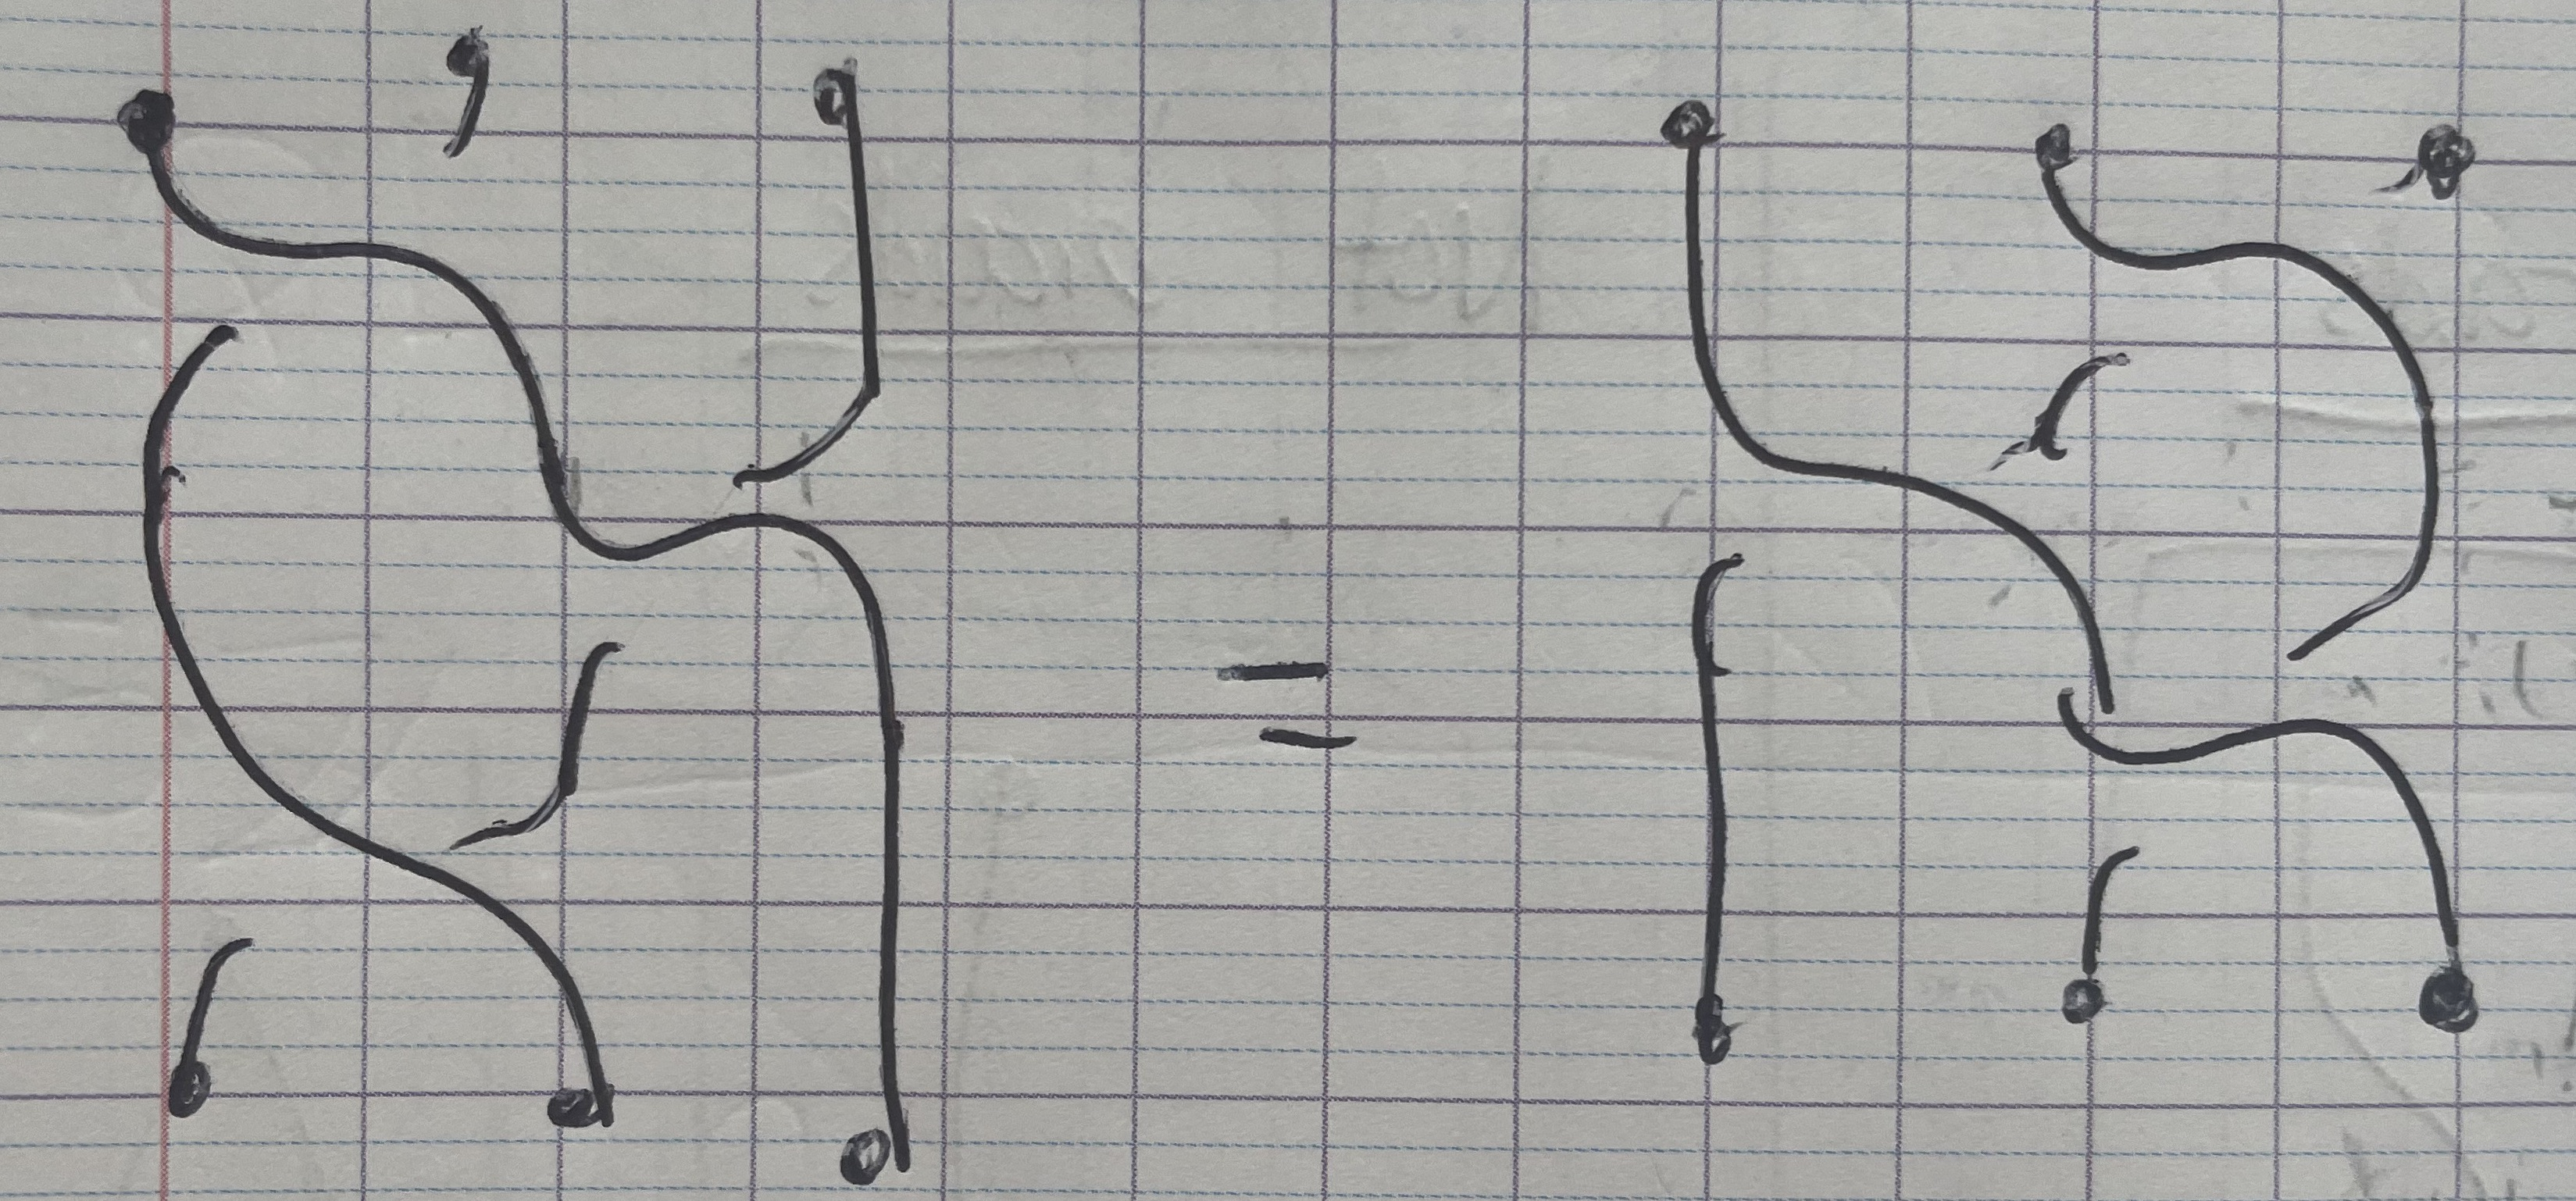
\includegraphics[scale=0.05]{yang-baxter}
\label{yang-baxter}
\end{center}
\end{figure}

Algebraically, this is the identity

$$\sigma_{i}\sigma_{i+1}\sigma_{i}=\sigma_{i+1}\sigma_{i}\sigma_{i+1}.$$

These relations we have obtained on the generators $\sigma_i$ of $B_n$, in fact, generate the space of all relations between the $\sigma_i$. This means that we have the following presentation for the group $B_n$:

$$B_n=\left<\left.\sigma_1,\sigma_2,...\sigma_{n-1}\right| \substack{ \sigma_{i}\sigma_{i+1}\sigma_{i}=\sigma_{i+1}\sigma_{i}\sigma_{i+1}\,\, \forall i, \\ \sigma_i\sigma_j=\sigma_j\sigma_i \,\,\forall |i-j|\geq 2}\right>.$$

We do not prove that this presentation of $B_n$ is correct, because our notions from topology are not rigorous enough to allow for such a proof. Instead, we take this presentation as an alternative algebraic definition of the braid group! At this point the lack of rigor in our treatment of braid groups and our lack of rigor in our treatment of defect trajectories cancel, giving us our first well-formed mathematical proposition. It records the fact that moving defects by braids acts on the stored information in the way we expect:

\begin{prop} Let $G$ be a finite group, and let $n\geq 1$ be an integer. The map

\begin{align*}
\rho_n: B_n &\xrightarrow{} \Sym\left(G^n\right)\\
\sigma_i &\mapsto \left((g_1... g_i, g_{i+1} ... g_n)\mapsto (g_1... g_{i+1}, g_{i+1}^{-1}g_i g_{i+1} ... g_n) \right)
\end{align*}

defines a homomorphism of groups between the braid group $B_n$ and the group $\Sym(G^n)$ of set-wise permutations of the Cartesian product $G^n$.
\end{prop}
\begin{proof} To prove this proposition we need to check that the group elements $\rho_n(\sigma_i)\in B_n$ satisfy the equations in the presentation of the braid group. The relation $\rho_n(\sigma_i)\rho_n(\sigma_j)=\rho_n(\sigma_j)\rho_n(\sigma_i)$ for $|i-j|\geq 2$ follows from the fact that $\rho_n(\sigma_i)$ and $\rho_n(\sigma_j)$ act on disjoint factors of $G$ in $G^n$.

The relation $\rho_n(\sigma_i)\rho_n(\sigma_{i+1})\rho_n(\sigma_i)=\rho_n(\sigma_{i+1})\rho_n(\sigma_i)\rho_n(\sigma_{i+1})$ follows evaluating both permutations on a sample element $(g_{i})_{i=1}^{n}\in G^n$ and verifying that they give the same result. Namely, we compute that

\begin{align*}
&\rho_n(\sigma_i)\rho_n(\sigma_{i+1})\rho_n(\sigma_i)(... g_{i}, g_{i+1},g_{i+2}...)\\
=&\rho_n(\sigma_i)\rho_n(\sigma_{i+1})(... g_{i+1}, (g_{i+1}^{-1}g_{i}g_{i+1}),g_{i+2}...)\\
=&\rho_n(\sigma_i)(... g_{i+1},g_{i+2}, (g_{i+2}^{-1}g_{i+1}^{-1}g_{i}g_{i+1}g_{i+2})...)\\
=&(... g_{i+2},(g_{i+2}^{-1}g_{i+1}g_{i+2}), (g_{i+2}^{-1}g_{i+1}^{-1}g_{i}g_{i+1}g_{i+2})...)\\
\end{align*}

and 

\begin{align*}
&\rho_n(\sigma_{i+1})\rho_n(\sigma_{i})\rho_n(\sigma_{i+1})(... g_{i}, g_{i+1},g_{i+2}...)\\
=&\rho_n(\sigma_{i+1})\rho_n(\sigma_{i})(... g_{i}, g_{i+2},g_{i+2}^{-1}g_{i+1}g_{i+2}...)\\
=&\rho_n(\sigma_{i+1})(... g_{i+2}, (g_{i+2}^{-1}g_{i}g_{i+2}),(g_{i+2}^{-1}g_{i+1}g_{i+2})...)\\
=&(... g_{i+2}, (g_{i+2}^{-1}g_{i+1}g_{i+2}), (g_{i+2}^{-1}g^{-1}_{i+1}g_{i}g_{i+1}g_{i+2}).
\end{align*}

Thus, the map $\rho_n$ is a well-defined group homomorphism.
\end{proof}

The final ingredient we need for our computer is the ability to create pairs of defects. Just like how a pair of defects with winding numbers $g$ and $g^{-1}$ could spontaneously fuse to give a defect with winding number $gg^{-1}=1$, the opposite process could start with a state with no defects and create a pair of defects with winding numbers $g$ and $g^{-1}$. We can now give the full list of operations which we require the experimenter to be able to perform for building a topological classical computer using ordered media:

\begin{enumerate}
\item The ability to create an ordered media state with no defects;
\item The ability to create pairs of defects with specified winding numbers;
\item The ability to perform defect-mobile deformations with specified defect trajectories;
\item The ability to measure the conjugacy class of the winding number associated to a defect.
\end{enumerate}

Before giving a general prescription of how to make a computer based on finite group $G$, we give a worked example. In this example, we use the group $G=A_5$ of all even permutations on five letters. We recall the basic features of the alternating group. It is a normal subgroup of the group $ \Sym(\{0,1,2,3,4\})$ of permutations on a five-element set. There is a canonical group homomorphism

$$\text{sign}:\Sym(\{0,1,2,3,4\})\xrightarrow{}\bZ_2$$

which sends a permutation in $\Sym(\{0,1,2,3,4\})$ to its sign, a $\bZ_2$-valued invariant. The alternating group $A_5$ is defined to be the kernel of this map, $A_5=\ker(\text{sign})$. In our context, the simplest way to define the sign is as follows. We observe that the symmetric group is the group obtained from taking the braid group and only remembering the endpoints of the braids, and not the exact way they bend around each other. Alternatively, the symmetric group is the group obtained from the braid group and identifying overcrossings with undercrossings. It is now a clear topological fact about braids that the number of overcrossings minus the number of undercrossings is an invariant of the braid - this can be also checked algebraically via the presentation we gave before. Thus, once overcrossings and undercrossings have been identifeid, we find that the total number of crossings is a $\bZ_2$-valued invariant. This is the sign.

The set of all permutations on five letters has $5!=120$ elements. Since $A_5$ is the kernel of a surjective map onto a two-element group, its order is $120/2=60$. We write the elements of $A_5$ using cycle notation. We denote by $(i_0,i_1...i_n)$ the cyclic permutation which sends $i_0$ to $i_1$, $i_1$ to $i_2$, all the way until $i_n$ which sends to $i_0$. The notation $(i_0...i_n)(j_0...j_m)$ refers to the composition of cycles, where first we permute by $(i_0...i_n)$ and then by $(j_0...j_m)$. With this notation in mind, we can move on to making the computer.

Our information is stored in pairs of defects whose overall winding number is trivial. In particular, we choose the following perscription for our binary zero and one states:

\begin{equation*}
\tikzfig{zero-and-one}
\end{equation*}

To encode $n$ bits of information we thus use $2n$ defects, put into pairs with opposite winding number. The fact that we can create a state with these pairs comes from points (1) and (2) of our assumptions on the experimenter.

We now describe the implementarion of logic gates on our computer. Our basic logic gate is the $\NAND$ gate, defined by the truth table

\begin{centering}
\[
\NAND(a,b)=
\begin{cases}
0 & a=b=1 \\
1 & \text{otherwise}.
\end{cases}
\]
\end{centering}

We implement the $\NAND$ gate as follows. We define a new state:

\begin{equation*}
\tikzfig{nc-state}
\end{equation*}

It is straightforward to verify that the following braid relation:

\begin{equation*}
\tikzfig{topological-and-gate}
\end{equation*}

That is, braiding $\ket{a}$ and $\ket{b}$ in the fashion described in the above picture around the non-computational state $\ket{*}$ has the effect of replacing the state $\ket{*}$ with $\ket{\NAND(a,b)}$.

Similarly, one can verify the following protocol for implementing the $\NOT$ gate, which flips the value of a bit from $0$ to $1$ and vice-versa:

\begin{equation*}
\tikzfig{topological-not-gate}
\end{equation*}

It is a well-known fact from computer science that the $\NAND$ gate and $\NOT$ gate can be used together to implement any boolean circuit. That is, every function $f:\{0,1\}^n\to \{0,1\}^n$ can be computed by taking the input bits, computing the $\NAND$ or $\NOT$ of these input bits in new registers, and the repeatedly computing more $\NAND$s and $\NOT$s in successive layers. A typical conversion from a standard boolean circuit to a topological circuit using $G=A_5$ woud look like this:

\begin{equation*}
\tikzfig{big-circuit}
\end{equation*}


The general method for making a topological classical computer follows in complete analogy from the case of $G=A_5$. To begin, one chooses a conjugacy class $C$ in $G$ with more than one element. This is possible whenever $G$ is non-abelian. Then, we choose two distinct elements $g_0,g_1$ in $G$. We define a computational state $\ket{0}$ to be a pair of defects with winding number $g_0$, $g_0^{-1}$ and we define $\ket{1}$ to be a pair of defects with winding number $g_1$, $g_1^{-1}$. Then, we find a scheme for implementing the $\NAND$ and $\NOT$ gates by braiding around some other defect, possibly including extra defects which are included just for the purpose of imeplementing the gate. We then use the NAND and NOT gates to implement all boolean circuits.

Let us analyse the above proposal in more detail. Suppose we want to implement the NAND gate of two bits $b_0$, $b_1$. The first step is to chose some group element $h\in C$, and initialize a pair of defects with winding numbers $h$, $h^{-1}$. Then, we procedure to braid the defects $\ket{b_0}$ and $\ket{b_1}$ around the $h,h^{-1}$ defect pair, as well as creating other auxillary defects and braiding them around the $h,h^{-1}$ pair. At the end of the process, the $h$ defect will have a new winding number, $f(g_{b_0},g_{b_1})hf(g_{b_0},g_{b_1})^{-1}$. Here, $f:\{0,1\}^2\to G$ is some function which is a product of the inputs $g_{b_0}$, $g_{b_1}$, their inverses, and fixed elements of $G$, any of which may appear multile times in the product. The condition we want is that

$$
f(g_{b_0},g_{b_1})hf(g_{b_0},g_{b_1})^{-1}=
\begin{cases}
g_0 & \text{if   }\NAND(b_0,b_1)=0\\
g_1 & \text{if }\NAND(b_0,b_1)=1.
\end{cases}
$$

Since $g_0,g_1$, and $h$ are all in the same conjugacy class, a function $f$ with the above property must exist. The only question is whether or not it is expressible as a product of the inputs $g_{b_0}, g_{b_1}$, their inverses, and fixed elements of $G$. If so, then a universal topological classical computing scheme is possible.


Clearly, if $G$ is abelian then the above scheme will not work. This is because we will not even be able to do the first step of the algorithm, which is to pick a conjugacy class with at least two elements. However, just being nonabelian is not enough. The group needs to be {\em sufficiently non-abelian} so that conjugation is powerful enough to implement the $\NAND$ gate. It turns out that a sufficient condition is that $G$ is a non-abelian {\em simple} group. We recall that a simple group is a group with no proper non-zero normal subgroups.

In this case we have the following important result, which paired with the above discussion immediately tells us that non-abelian simple groups can be used to make a universal classical computer:

\begin{thrm}[Mochon; Maurer-Rhodes]\label{mochon-theorem} Let $G$ be a non-abelian simple group. Every function $f(g_1,g_2...g_n):G^n\to G$ can be expressed as the product of the inputs $\{g_i\}$, their inverses $\{g_i^{-1}\}$, and fixed elements of $G$, any of which may appear multiple times in the product.
\end{thrm}
\begin{proof} The original proof is in a paper of Maurer-Rhodes \cite{maurer1965property}. The connection to topological computing was dicovered in \cite{mochon2003anyons}, where a new constructive proof was also given.
\end{proof}

\begin{rem}
In light of Theorem \ref{mochon-theorem}, it is natural to see why we chose the group $A_5$ in our example of topological classical computing. The group $A_5$ of order $60$ is the smallest non-abelian simple group! This concludes our overview of the subject.
\end{rem}

$\newline\newline$

\large \textbf{Exercises}:\normalsize

\begin{enumerate}[\thesection .1.]

\item Verify the protocol for copying the value of a bit using a $G=A_5$ topological classical computer,
\begin{equation*}
\tikzfig{cloning-gate}
\end{equation*}

where

\begin{equation*}
\tikzfig{NC-state-reprise}
\end{equation*}

\item \Note{show that nilpotent $\implies$ polynomial growth? Can reference the more general picture of size of braid group images.}

\item \Note{definition of the braid group as a fundamental group.}

\item \Note{It is a theorem that for any non-solvable finite group $G$, there exists a normal subgroup $P$ of $G$ and a normal subgroup $N$ of $P$ such that $P/N$ is simple. Use this to deduce a universal classical computation scheme based on any non-solvable group.}
\end{enumerate}


